%!TEX root = ../thesis.tex
\chapter{Numerical investigations\label{sec: numerics}}
We have now established multiple schemes for approximating fluid queues which are suitable for approximating the performance measures of fluid-fluid queues derived in \cite{bo2014}. This chapter investigates, numerically, various aspects of the approximation schemes. Throughout, we compare the QBD-RAP scheme (from Chapter~\ref{sec: construction and modelling}), the discontinuous Galerkin scheme (as described in Chapter~\ref{ch:galerkin}, with and without slope limiting), and the \emph{spatially-coherent uniformisation} scheme introduced by \cite{bo2013}. 

The performance of the discontinuous Galerkin scheme has been well-studied in some contexts (\cite{c99}, \cite{nodalDGBook}~Section~5.5), and it is well-known that the discontinuous Galerkin scheme performs remarkably well on problems with smooth solutions. Here, we mostly focus on investigating the numerical performance of the schemes on problems with non-smooth solutions. The purpose is to emphasise the probabilistic interpretation and positivity-preserving properties of the QBD-RAP scheme. In the stochastic modelling community it is common to have problems with discontinuities, such as non-smooth initial conditions, hence the type of problems we investigate in this chapter are of relevance. As we will see (in Section~\ref{sec: transient approx}), even if a fluid-queue is initialised with a smooth initial density, the boundary dynamics may induce transient discontinuities or non-smooth behaviour into the problem. A very specific set of conditions on the initial density and point masses must hold for the transient distribution to remain continuous as it evolves over time \citep{bo2014,boz2022}. Further, it is possible that discontinuities are present in the performance measures of fluid-fluid queues (see, for example, Section~\ref{sec: ffq num}). Limiting distributions of fluid queues are smooth, however.

The experiments demonstrate that the DG scheme can perform extremely well when the true solution is sufficiently smooth. However, when discontinuities are present in the true solution, the DG scheme can lead to approximate solutions which are oscillatory and this may lead to approximate solutions which violate the axioms of probability, such as approximations to PDFs which take negative values (equivalently, approximations to CDFs which are non-increasing), and in the worst cases, approximations to CDFs which take values outside \([0,1]\). Hence, there is a need for schemes which ensure the axioms of probability are maintained. 

By design, the QBD-RAP scheme, uniformisation scheme, and DG schemes with slope limiting, produce approximations which obey the axioms of probability, i.e. produce approximations to PDFs which are non-negative, and CDFs which are non-decreasing, and \([0,1]\)-valued.  

We implement two slope limited DG schemes, the DG-lim and DG-lin-lim scheme, which we describe in more detail in the next section. The numerical experiments demonstrate that the DG-lim scheme does not lead to a viable approximation scheme in the presence of discontinuities, while the DG-lin-lim scheme results in a relatively performant approximation scheme for the discontinuous problems considered here. In general, the QBD-RAP scheme performs similarly to the DG-lin-lim scheme, while the uniformisation scheme is a viable approximation method, but produces larger errors than the QBD-RAP and DG-lin-lim scheme, for the examples considered here. When slope limiting is used, the resultant approximation is at best linear around discontinuities. Moreover, there is a computational cost in applying a limiter (or filter), which could be significant, particularly if many initial conditions are to be considered. In contrast, for the uniformisation and QBD-RAP, the approximate solution is guaranteed to produce positive probabilities without any post-processing or extra computation. 

Although we have been unable to supply a rigorous argument to show that we can use the DG approximation to the generator of a fluid queue to approximate performance measures of fluid-fluid queues, such as the operator \(\mathbb \Psi\), we can rely on the intuition that substituting the DG approximation for the true operator \emph{should} give reasonable results, and further, \emph{assume} that the resulting approximations are polynomial.

On the other hand, using the stochastic approximations (QBD-RAP or uniformisation), results in rigorously defined operators as proved in \cite{bgnp2021}.

In summary, the QBD-RAP and uniformisation schemes are the only two schemes which result in rigorously defined approximations, preserve the axioms of probability, and, of the two, the numerical experiments demonstrate that the QBD-RAP method is superior. 

\section{Preliminaries}
Before presenting the results of the experiments, we need to describe some aspects of the approximation schemes in more detail, which we now proceed to do. 

The main focus of the numerical experiments is on the error as the number of basis functions per cell is increased. In the numerical experiments the number of basis functions used to approximate the solutions is the same on all cells and the number of basis functions on a cell (and hence all cells) is referred to as the \emph{dimension} of the scheme. For the discontinuous Galerkin scheme, the dimension of the scheme means is the number of polynomial basis functions used to approximate the solution within each cell. For example, if we use 3 basis functions in the discontinuous Galerkin scheme, we approximate the solution by 3 linearly independent quadratics on each cell and hence the approximation is a quadratic on each cell. For the QBD-RAP scheme, the dimension of the scheme is the order of the CME distribution used to construct the scheme. To make a comparable equivalent for the uniformisation scheme, we divide each cell into smaller sub-cells over which we approximate the solution. That is, for a dimension \(p\) uniformisation scheme we divide each cell into \(p\) sub-cells. Equivalently, we may think of a dimension \(p\) uniformisation scheme as using \(p\) piecewise constant functions to approximate the solution on each cell. For all schemes (DG, QBD-RAP and uniformisation), if we construct a dimension \(p\) approximation, there are \(K\) cells, \(N\) phases and \(c_i\neq 0\) for all \(i\in\calS\), then the resulting approximation to the generator \(\mathbb B\) is a square matrix of dimension \(pKN + N\).\footnote{There are \(pK\) basis functions for each phase which approximate the solution on the interior of the domain, hence \(pKN\) basis functions in total, plus an additional \(N\) dimensions to capture boundary conditions.} In this sense each approximation scheme leads to matrices of the same order (although not necessarily the same number of non-zero elements). 

We investigate two slope-limited schemes. In the scheme we refer to the \emph{DG-lim} scheme, we use a DG scheme of dimension \(p\) and apply the Generalised MUSCL slope limiter as described in Section~\ref{sec: slope limiting}. In the \emph{DG-lin-lim} scheme, we follow the construction described in Section~\ref{sec: anoth pos pres}, which is effectively a DG scheme with cells of width \(2\Delta/(p+1)\), for \(p=1,3,5,...,21\), and a basis of dimension \(2\) (linear) on each cell, with an upwind flux, and we apply the Generalised MUSCL limiter. Thus, the DG-lin-lim scheme uses \(p+1\) basis functions to represent the solution on each of the original cells \(\calD_k\), and we define the dimension of the scheme to be \(p+1\). In the presence of discontinuities, slope-limiting forces the approximation to be linear, i.e.~an order~1 polynomial, around the discontinuity. For DG schemes of dimension greater than 2 with a slope limiter and in the presence of discontinuities, the ability of the scheme to represent higher-order polynomials is not well-utilised as the slope limiter forces the solution to be linear anyway. The DG-lin-lim scheme recognises this and instead of using higher-order polynomials, uses piecewise-linear functions and smaller cell widths to approximate the solution. 

%The concept of slope-limiting originates in the context of numerically integrating (typically with respect to a \emph{time} variable) a so-called \emph{semi-discrete system}, as we do in Section~\ref{sec: transient approx}. However, approximating the operator \(\mathbb\Psi\) of a fluid-fluid queue amounts to solving an implicit matrix-equation and there is no concept of numerical integration with respect to time. Hence, the concept of slope-limiting, it is not directly transferable. One could process the initial condition and post-process the solution with a limiter. However, there are possibly better choices for this post-processing, such as filtering, \citep[Section~5.6.1]{nodalDGBook}. One could also view the composition of the DG operator and the limiting operator as one, but the result is a non-linear operator which is of no use for simplifying the Riccati Equation which characterises \(\mathbb \Psi\). Considering there is no theory on the use of the DG scheme to approximate \(\mathbb \Psi\) and hence the resultant approximation is not rigorously-defined, the author does not know if the use of a limiter in this context is possible. 

To keep the content of this chapter contained, we do not investigate all aspects of the schemes. For each numerical experiment we keep the number of cells, \(K\) (equivalently, the cell size, \(\Delta\)), fixed for the DG and QBD-RAP schemes. As part of deriving a discontinuous Galerkin scheme, one needs to choose the \emph{numerical flux} which is used to approximate the transition of density from one cell to the next \citep{nodalDGBook}. We investigate schemes with an upwind flux only. We do not investigate filtering for the DG scheme.

For schemes which require us to integrate over time we do not investigate the stability of the schemes with respect to the \(t\)-step-size, or the time-integration scheme itself (where required). Instead, we fix the time-integration step size for each numerical experiment at a suitably small value to obey a certain stability criterion (a CFL-like condition, \citep[Section~4.8]{nodalDGBook}). Moreover, we always implement the strong stability preserving Runge-Kutta method of order 4 with 5 stages (\cite{sr2002}, \cite{nodalDGBook}~Section~5.7, see also Section~\ref{sec: time integration}), which is claimed to introduce no more oscillations into the solution as we integrate over time. 

Where a slope limiter is implemented, we implement the \emph{Generalised MUSCL} limiter (\cite{c99}, \cite{nodalDGBook}~Section~5.6.2, see also Section~\ref{sec: slope limiting}). 

In this chapter, all the error plots are on a \(\log_{10}\)-\(\log_{10}\) scale. If the error function takes the form \(error = \beta_0^* p^{\beta_1}\), where \(p\) is the dimension of the scheme, then the \(\log_{10}\)-\(\log_{10}\) will show a linear trend since \(\log_{10}(error) = \beta_0 + \beta_1 \log_{10}(p)\), where \(\beta_0=\log_{10}(\beta_0^*)\). Where relevant, to estimate the asymptotic rate of convergence, \(\beta_1\), we estimate the slope of the line \(\log_{10}(error) = \beta_0 + \beta_1 \log_{10}(p)\) using ordinary least squares and the last eight data points of each line. The estimated linear trends are plotted and the slope of the line is displayed to the right of the plot. 

The structure of this chapter is as follows. In Section~\ref{sec: recon num} we compute approximations to various initial conditions for the different schemes and observe their performance which allows us to investigate the performance of the reconstruction methods without considering a specific model or any dynamics. In Section~\ref{sec: wave num} we investigate travelling wave problems with various initial conditions. For the travelling wave problem the dynamics are deterministic, which means that the solution is known, and we do not need to resort to simulation as a \emph{ground-truth}. Furthermore, the travelling wave problems allow us to investigate the ability of the schemes to approximate the flow of probability across cells without any stochastic dynamics. Next, we investigate a simple fluid queue with two phases. Section~\ref{sec:stat} investigates approximations to the limiting distribution of the queue, Section~\ref{sec: transient approx} investigates approximations to the transient distribution of the queue for two initial conditions, and Section~\ref{sec: hit approx} investigates approximations the first hitting time of the fluid level on the set \(\{0,1\}\). Lastly, we apply the approximation methods to a fluid-fluid queue in Section~\ref{sec: ffq num}, compute approximations to \(\mathbb \Psi\) and ultimately, approximate the distribution of \(\{(X(\zeta_{W}(\{0\})),\varphi(\zeta_{W}(\{0\})))\}\) at time \(\zeta_{W}(\{0\})\) at which \(\{\dot W(t)\}\) first returns to \(0\). 


\paragraph{On the application of the QBD-RAP approximation to approximating operators of fluid-fluid queues.}
A few remarks about applying the QBD-RAP approximation to approximate fluid queues and operators of fluid-fluid queues from \cite{bo2014} are in order. 

Despite the construction of the QBD-RAP in Chapter~\ref{sec: construction and modelling} and the proof of convergence to the fluid queue spanning Chapters~\ref{sec: conv} and \ref{ch: global results} being relatively technical, the actual computations involved are relatively simple once we have the generator of the QBD-RAP. Construction of the generator matrix of the QBD-RAP, \(\bs B\), is a matter of obtaining the parameters \(\bs\alpha,\,\bs S\) and \(\bs s\) of a concentrated matrix exponential distribution from \cite{hht2020}, computing the matrix \(\bs D\) as in the last part of Section~\ref{sec:kkkrjrjrjjrj}, then assembling the parameters into the tridiagonal form of the generator as in (\ref{eqn: BBBB})-(\ref{eqn: BBBB3}) and including boundary conditions as in (\ref{eqn: BBBBbndry})-(\ref{eqn: BBBBbndry2}). The initial vector of the QBD-RAP, \(\bs a=(\bs a_{k,i})_{i\in\calS,k\in\mathcal K}\), can be constructed as discussed in Section~\ref{sec: initial conditions}, perhaps using numerical integration depending on the choice of initial condition. After constructing the generator and initial condition, approximations to the fluid queue can be obtained relatively easily. For example, the expected orbit positions in each phase and level, \(\mathbb E[\bs A(t)1(L(t)=\ell, \phi(t)=i)]\), are found by computing 
\[(\mathbb E[\bs A(t)1(L(t)=\ell, \phi(t)=i)])_{i\in\calS, \ell \in\mathcal K}=\bs a \exp(\bs Bt),\]
which, in this chapter, is computed numerically via the SSPRK integration scheme in Section~\ref{sec: time integration}. The approximation to the transient density is obtained from \(\mathbb E[\bs A(t)1(L(t)=\ell, \phi(t)=i)]\) as discussed in Section~\ref{sec: closing}.

To approximate operators of fluid-fluid queues with the QBD-RAP  we need to approximate the operator \(\mathbb R\), defined in Lemma~\ref{lemma: D(s)}. Recall from Section~\ref{sec: approx r}, in the context of the DG scheme we could approximate \(\mathbb R\) as a projection. In the context of the QBD-RAP scheme it is less clear how one can approximate \(\mathbb R\), in general. If the rate functions \(r_i(x)\) are piecewise constant with \(r_i(x)=r_i^k\) on cell \(\calD_{k,i}\), then a suitable approximation for \(\mathbb R^k_i\) is \(1/|r_i^k|\bs I_{p}\), a diagonal matrix with \(1/|r_i^k|\) down the diagonal -- this is the case in the numerical experiments in Chapter~\ref{sec: numerics}. For more general cases we could consider approximating \(r_i(x)\) by a piecewise constant function, then apply the method above.

Next, the approximation \(\bs \Psi\) is computed by solving the matrix Riccati equation 
\begin{align}\label{eqn:RiccatiPsi2222aa}
    \bs D^{+-}
+ \bs \Psi   \bs D^{-+}\bs \Psi
+   \bs D^{++}\bs \Psi
+ \bs \Psi  \bs D^{--}
= \bs 0,
\end{align}
where 
\[\bs D^{mn} = \bs{R}^m (\bs{B}^{mn} + \bs{B}^{m0}(\bs B^{00})^{-1}\bs{B}^{0n}), \, m,n\in\{+,-\},\]
and \(\bs{B}^{mn},\, m,n\in\{+,-,0\}\) are matrices of parameters extracted from the QBD-RAP which approximate \(\mathbb B^{mn}\). For example, \(\bs B^{+-}\) is obtained by extracting all the elements of \(\bs B\) which correspond to starting in phase \(i\) in level \(k\) and ending in phase \(j\) in level \(\ell\) and have \(r_i(x)>0\) for \(x\in\calD_{k,i}\) and \(r_j(x)<0\) for \(x\in\calD_{\ell,j}\). Given the stochastic interpretation of the QBD-RAP scheme, and assuming the rate functions \(r_i(x)\) are piecewise constant with \(r_i(x)=r_i^k\) on each cell \(\calD_{k,i}\), the QBD-RAP approximation of the fluid-fluid queue forms a RAP-modulated fluid process \citep{p2019,bgnp2021}. Hence, the approximation \(\bs \Psi\) has a stochastic interpretation in terms of the first-return operator of the RAP-modulated fluid process. This is important. Equation (\ref{eqn:RiccatiPsi2222aa}) determines, but does not define \(\bs \Psi\). When we use the DG scheme to approximate \(\mathbb \Psi\) we still solve (\ref{eqn:RiccatiPsi2222aa}) (with the DG approximation to the generator \(\mathbb B\)), however, this does not define what the solution means in terms of the fluid-fluid queue (other than it is the solution to (\ref{eqn:RiccatiPsi2222aa})). In comparison, there is a rigorous definition of \(\bs \Psi\) when the QBD-RAP scheme is used in the approximation \citep{p2019,bgnp2021}. 

By Proposition~4.3 of \cite{p2019}, for the QBD-RAP scheme the approximation \(\bs \Psi\) has the property \(\bs \Psi \bs 1=\bs 1\) as long as the event that level process of the RAP-modulated fluid returns to \(0\) in finite time occurs with probability 1. 

Third, note that unlike the positivity preserving DG schemes which use slope limiting which are not linear operators in the presence of oscillations, the operator obtained via the QBD-RAP approximation scheme is linear.

{Lastly, a comment on expected accuracy of the QBD-RAP scheme.} For \(p\) odd, \cite{hht2020} estimate that the variance of the class of CMEs decreases at order \(1/p^{2.14}\) asymptotically. Hence, we might expect the rate of convergence of the QBD-RAP scheme to be approximately order \(1/p^2\) for certain problems. This is in line with the positivity preserving DG scheme mentioned in~\ref{sec: anoth pos pres}. %The justification for considering representations of odd orders only is that the variance of CME representations of orders \(2p\) and \(2p-1\) are relatively similar and therefore have similar abilities to represent the delta function \citep{hht2020}. Hence, if we construct a QBD-RAP approximation with a representation of order \(2p\) we expect it to perform only marginally better than an approximation constructed with representations of order \(2p-1\). However, the computational cost of the latter is lower, so we opt for the order \(2p-1\) representation. 


% \chapter{Old}
% We have now established multiple schemes for approximating fluid queues which are suitable for approximating the performance measures of fluid-fluid queues derived in \cite{bo2014}. In this chapter we numerically investigate various aspects of the approximation schemes. Throughout, we compare the QBD-RAP scheme (from Chapter~\ref{sec: construction and modelling}), the discontinuous Galerkin scheme (as described in Chapter~\ref{ch:galerkin}), and the spatially-coherent uniformisation scheme introduced by \cite{bo2013}. %Recall that the uniformisation scheme is equivalent to a discontinuous Galerkin scheme with a constant basis function in each cell, which is also equivalent to the finite-volume scheme with an upwind flux. 
% Recall that, due to their stochastic interpretation, the uniformisation and QBD-RAP schemes are positivity preserving. 

% The main focus of our numerical experiments is on the convergence properties as the number of basis functions is increased. For simplicity, the number of basis functions is kept constant across all cells. We refer to the number of basis functions on a cell \(k\) as the \emph{dimension} and consider dimensions \(p=2r+1\) for \(r=0,1,2,3,...,10\). For discontinuous Galerkin scheme, increasing the dimension of the scheme means increasing the number of polynomial basis functions used to approximate the solution within each cell. E.g.~if we use 3 basis functions in the discontinuous Galerkin scheme, we approximate the solution by a quadratic on each cell. For the QBD-RAP scheme, increasing the dimension of the scheme means increasing the order of the CME distribution used to construct the scheme. To make a comparable equivalent for the uniformisation scheme with a fixed cell size we divide each cell into smaller sub-cells over which we approximate the solution. I.e.~for a dimension \(p\) uniformisation scheme we divide each cell into \(p\) sub-cells. Equivalently, we may think of a dimension \(p\) uniformisation scheme as using \(p\) piecewise constant functions to approximate the solution on each cell. For all schemes (DG, QBD-RAP and uniformisation), if we construct an order \(p\) approximation, there are \(K\) cells, \(N\) phases and \(c_i\neq 0\) for all \(i\in\calS\), then the resulting approximation to the generator \(\mathbb B\) is a matrix of dimension \(pKN + N\). In this sense each approximation scheme leads to matrices of the same size (although not necessarily the same number of non-zero elements). 

% To keep the content of this chapter contained, we do not investigate all aspects of the schemes. For each numerical experiment we keep the cell size, \(\Delta\), fixed for the DG and QBD-RAP schemes. As part of deriving a discontinuous Galerkin scheme, one needs to choose the \emph{numerical flux} which is used to approximate the transition of density from one cell to the next \citep{nodalDGBook}. We investigate schemes with an upwind flux only. For schemes which require us to integrate over time we do not investigate the stability of the schemes with respect to the \(t\)-step-size, or the time-integration scheme itself (where required). Instead, we fix the time-integration step size for each numerical experiment at a suitably small value to obey a certain stability criterion (a CFL-like condition, \citep[Section~4.8]{nodalDGBook}). Moreover, we always implement the strong stability preserving Runge-Kutta method of order 4 with 5 stages (\cite{sr2002}, \cite{nodalDGBook}~Section~5.7, see also Section~\ref{sec: time integration}), which claims to introduce no more oscillations into the solution as we integrate over time. 

% For some numerical experiments we implement the discontinuous Galerkin scheme with and without a slope-limiter implemented (\cite{c99}, \cite{nodalDGBook}~Section~5.6.2, see also Section~\ref{sec: slope limiting}). The slope limiter avoids oscillations and negative solutions. However, we note that in the context of approximating the operator \(\mathbb\Psi\) for a fluid-fluid queue, it is not obvious how one might apply the concept of slope-limiting, other than to post-process the solution with a limiter or filter. Even when slope limiting is possible, the resultant approximation is at best linear around discontinuities. Moreover, there is a computational cost in applying a limiter, which could be significant, particularly if many initial conditions are to be considered. In contrast, for the uniformisation and QBD-RAP the approximate solution is guaranteed to produce positive probabilities without any post-processing or extra computation.

% Where a slope limiter is implemented, we implement the \emph{Generalised MUSCL} limiter (\cite{c99}, \cite{nodalDGBook}~Section~5.6.2, see also Section~\ref{sec: slope limiting}). We investigate two schemes with slope limiting. In the first scheme, which we refer to the \emph{DG-lim} scheme, we use a DG scheme of dimension \(p\) and apply the Generalised MUSCL slope limiter as described in Section~\ref{sec: slope limiting}. In the second scheme, which we refer to as the \emph{DG-lin-lim} scheme, we follow the construction described in~\ref{sec: anoth pos pres}, which is effectively a DG scheme with cells of width \(2\Delta/(p+1)\), for \(p=1,3,5,...,21\), and a basis of dimension \(2\) (linear) on each cell, with an upwind flux, and we apply the Generalised MUSCL limiter. Thus, the DG-lin-lim scheme uses \(p+1\), \(p=1,3,5,...,21\), basis functions to represent the solution on each of the original cells \(\calD_k\), and we define the dimension of the scheme to be \(p+1\). We do not investigate filtering for the DG scheme.

% The performance of the discontinuous Galerkin scheme has been well-studied in some contexts (\cite{c99}, \cite{nodalDGBook}~Section~5.5), and it is well-known that the discontinuous Galerkin scheme performs remarkably well on problems with smooth solutions. Here, we mostly focus on investigating the numerical performance of the schemes on problems with non-smooth solutions. The purpose of this is to emphasise the positivity-preserving properties of the QBD-RAP scheme. In the stochastic modelling community it is very common to have problems with discontinuities, such as a non-smooth initial conditions. As we will see (in Section~\ref{sec: transient approx}), even if a fluid-queue is initialised with a smooth initial density, the boundary dynamics may induce transient discontinuities or non-smooth behaviour into the problem. A very specific set of conditions on the initial density and point masses must hold for the transient distribution to remain continuous as it evolves over time \citep{bo2014,bop2020}. Further, it is possible that discontinuities are present in the performance measures of fluid-fluid queues (see, for example, Section~\ref{sec: return approx}). Limiting distributions of fluid queues are smooth, however.

% As we shall see, if the solution is smooth, then the DG scheme is highly-effective and exhibits rapid convergence to the solution as the number of polynomial basis functions is increased. However, when the solution is non-smooth oscillations and negative approximations may occur when using the discontinuous Galerkin scheme, leading to nonsense solutions. In these cases, the QBD-RAP and DG-lin-lim approximations perform relatively well compared to the other positivity preserving schemes investigated. 

% Lastly, before we start the numerical investigation, note that all the following error plots are on a \(\log_{10}\)-\(\log_{10}\) scale. If the error function takes the form \(error = \beta_0^* p^{\beta_1}\), where \(p\) is the dimension of the scheme, then the \(\log_{10}\)-\(\log_{10}\) will show a linear trend; \(\log_{10}(error) = \beta_0 + \beta_1 \log_{10}(p)\), where \(\beta_0=\log_{10}(\beta_0^*)\). Where relevant, to estimate the asymptotic rate of convergence, \(\beta_1\), we estimate the of the line \(\log_{10}(error) = \beta_0 + \beta_1 \log_{10}(p)\) using ordinary least squares and the last eight data points on each plot. We plot the estimated lines of best fit and quote their slope to the right of the plots. 

% The structure of this chapter is as follows. In Section~\ref{sec: recon num} we compute approximations to various initial conditions for the different schemes and observe their performance. This allows us to investigate the performance of the reconstruction methods without considering a specific model or any dynamics of the problem. In Section~\ref{sec: wave num} we investigate travelling wave problems with various initial conditions. For the travelling wave problem the dynamics are deterministic, which allows us to investigate the ability of the schemes to approximate the flow of probability across cells without any stochastic dynamics. Next, we investigate a simple fluid queue with two phases. Section~\ref{sec:stat} investigates the ability of the schemes to approximate the limiting distribution of the model, Section~\ref{sec: transient approx} investigates the ability of the schemes to approximate the transient distribution of the model for two initial conditions, and Section~\ref{sec: return approx} investigates the ability of the schemes to approximate the first hitting time of the fluid level on the boundary of the interval \([0,1]\). Lastly, we apply the approximation methods to a fluid-fluid queue in Section~\ref{sec: ffq num} and approximate the distribution of \(\{(X(t),\varphi(t))\}\) at the time at which \(\{W(t)\}\) first returns to \(0\).  

% THE STRUCTURE OF THE CHAPTER IS AS FOLLOWS. 

% 1. FUNCTION APPROX./RECONSTRUCTION

% 2. 1d wave eqn

% 3. limiting DISTRIBUTIONS
	% i. SIMPLER
	% ii. MORE COMPLEX
	
% 4. TRANSIENT DISTRIBUTIONS 
	% i. SIMPLER
	% ii. MORE COMPLEX

% 5. HITTING TIMES 
	% i. SIMPLER
	% ii. MORE COMPLEX

% 6. FLUID-FLUID QUEUES

% 7. CONCLUDING REMARKS 

\section{Function approximation/reconstruction}\label{sec: recon num}
We start our investigation by looking at how well the schemes perform at approximating an initial condition. By approximating the initial condition only, we aim to investigate the performance of the approximation schemes without any dynamics.

For the discontinuous Galerkin method, we project the initial condition on to the set of polynomial basis functions which define the scheme, for the spatially-coherent uniformisation scheme, we look at the sub-cell averages of the initial condition, and for the QBD-RAP scheme, we compute the initial vector for the approximation, then reconstruct the solutions as described in Sections~\ref{sec: initial conditions} and~\ref{sec: closing}. For the purposes of approximation and reconstruction for the QBD-RAP scheme we must orientate the initial condition in a positive or negative direction; here we suppose that the initial conditions belong to a positive phase. First we investigate the three closing vectors from Section~\ref{sec: closing} which we can use for the reconstruction in the QBD-RAP scheme. From the investigation, we decide to use the closing vector (\ref{eqn:5462}) throughout the rest of the chapter.

In this section we consider approximating initial conditions over a single cell of width \(\Delta = 1\). To numerically evaluate integrals arising in the approximation step (inner products and cell averages) we use a trapezoidal rule with 10,001 function evaluations. Similarly, we use 10,001 function evaluations to approximate \(L^p\) errors, and also as a finite set of points over which to compute the Kolmogorov-Smirnov (KS) statistics. 

% First we briefly investigate the possible choices of closing operators as introduced in Section~\ref{sec: closing}. 

\subsection{QBD-RAP closing operators}\label{sec: closing vecs numerics}
We investigate the three closing operators introduced in \ref{sec: closing}. For convenience, we restate the three closing operators from Section~\ref{sec: closing} here. The unnormalised closing vector, 
\begin{align}
	\bs a {\bs v}(x) &= \bs a e^{\bs Sx}\bs s.\tag{\ref{eqn: alal}}
	%\\\bs a {\bs v}_-(x-y_\ell) &= \bs a e^{\bs S(x-y_{\ell})}\bs s,\label{eqn:ndaenf}
\end{align} 
A normalised version of the closing operator in Equation~(\ref{eqn:546}), with the normalised version given by 
\begin{align}
	\bs a {\bs v}(x) &= \cfrac{\bs a \left(e^{ \bs{S}x} \bs s + e^{ \bs{S}(2\Delta-x)} \bs s\right)}{1-\bs a e^{\bs S 2\Delta}\bs e}. \tag{\ref{eqn: nonlin}}
\end{align} 
We refer to the closing operator in (\ref{eqn: nonlin}) as the \emph{non-linear normalised} closing operator.\footnote{Technically we have not yet proved that the \emph{non-linear} normalised closing operator leads to a convergent approximation scheme.} The third closing vector we investigate is given by 
\begin{align}
	\bs a {\bs v}(x) &= \bs a \left(e^{ \bs{S}x} \bs s + e^{ \bs{S}(2\Delta-x)}\right)\left[I-e^{S2\Delta}\right]^{-1} \bs s,\tag{\ref{eqn:5462}}
\end{align}
which we refer to as the \emph{normalised} closing operator. 

\begin{example}\label{ex: another example}
	\begin{figure}[h]
		\centering
		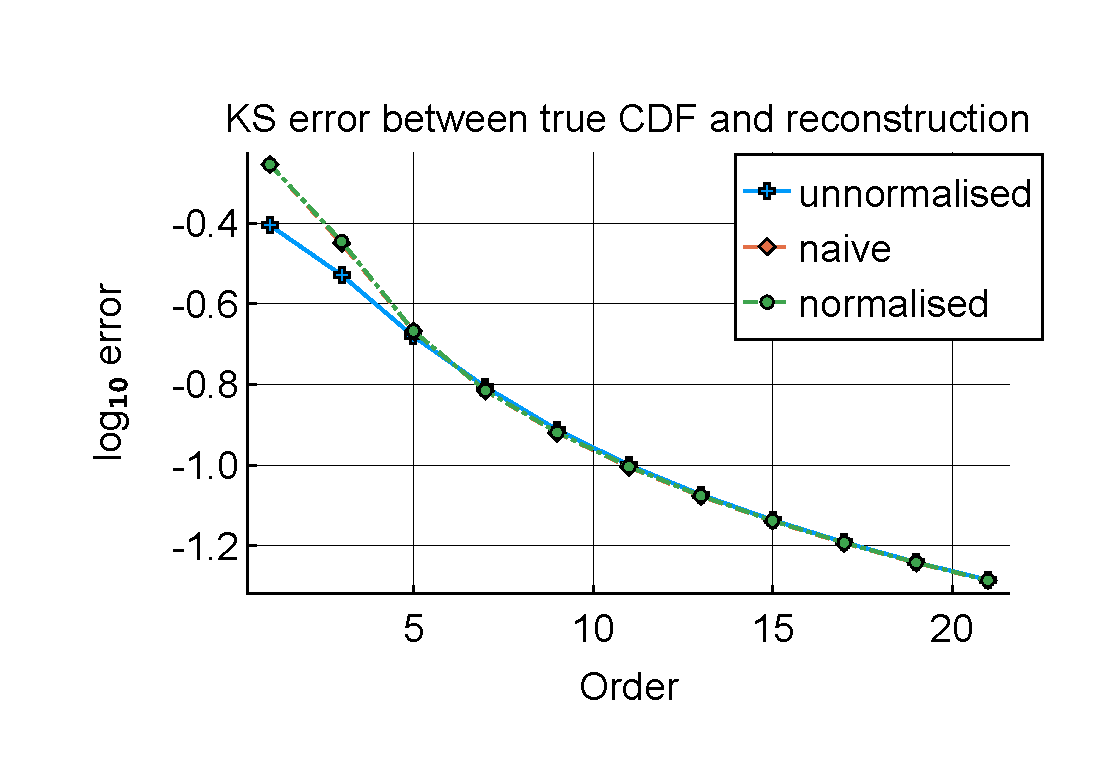
\includegraphics[width=0.5\textwidth,trim={0.5cm 0.8cm 0.2cm 1.25cm},clip]{chapter6/figs/qbdrap_closing_vec/fun2/ks_error_formatted.pdf}%
		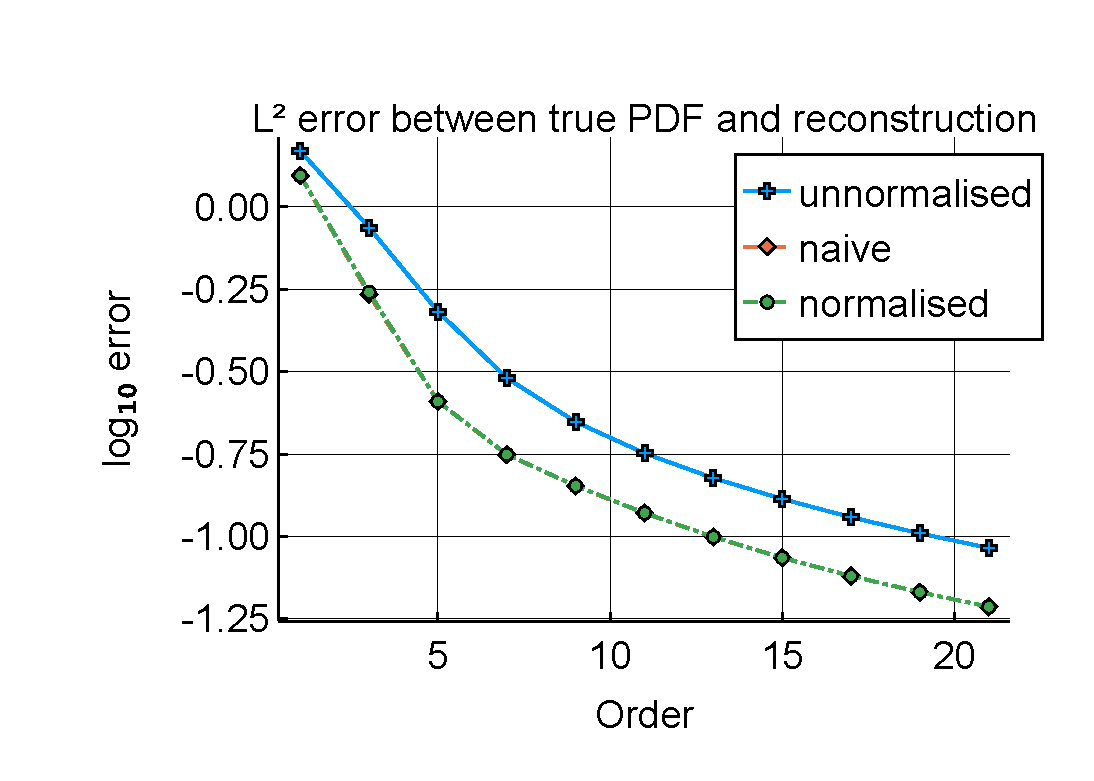
\includegraphics[width=0.5\textwidth,trim={0.5cm 0.8cm 0.2cm 1.25cm},clip]{chapter6/figs/qbdrap_closing_vec/fun2/l2_pdf_error_formatted.pdf}
		\caption{KS error (left) and \(L^2\) error of the PDF (right) of Example~\ref{ex: another example} for the three closing vectors considered; unnormalised (green solid line), non-linear normalised (blue dashed line) and normalised (orange dash-dotted line). The error curves of the non-linear normalised and normalised closing vectors are almost coincident. The black dotted lines are linear least-squares fits to the last 8 data points and the slopes of the least square lines are written next to the last point.}%To estimate the asymptotic rate of convergence, we fit a linear model of \(\log_{10}(error) = \beta_0 + \beta_1\log_{10}(Dim)\) to the the last 6 data points on the curves above, which corresponds to a rate of convergence \(error \propto N^{-\beta_1}\). The estimate of \(\beta_1\) was approximately -1.0 in all cases.}
		\label{fig: fun 2 ks error qbdrap closing vecs}
	\end{figure} 
	%\exampleFloatBarrier
	First consider approximating the initial condition with density function \(2\times 1(x<0.5)\), where \(1(\cdot)\) is the indicator function. In the left-hand side of Figure~\ref{fig: fun 2 ks error qbdrap closing vecs} we plot the Kolmogorov-Smirnov error between the true CDF and the CDF constructed via the QBD-RAP approximation with the three different closing vectors. Interestingly, in this case, the unnormalised closing operator outperforms the other two at low dimensions. In this case, it just so happens that the error due to truncation of the unnormalised reconstruction constructively interferes with other errors to cause the error to be lower at low dimensions for the unnormalised scheme. 
	
	Figure~\ref{fig: fun 2 ks error qbdrap closing vecs} also shows that the non-linear normalised and normalised closing operators perform very similarly -- this is the case throughout much of this section. The difference between the non-linear normalised and normalised closing operators is how they treat mass in the tail of a matrix exponential distribution (from \(2\Delta\) onward). Intuitively, there should be very little mass in the tail of the distribution as we are using concentrated matrix exponential distributions in the reconstruction. 

If we instead look at the \(L^2\) error between the true PDF and the reconstructions in Figure~\ref{fig: fun 2 ks error qbdrap closing vecs} (right), then we see that the unnormalised reconstruction performs the poorest. Figure~\ref{fig: fun 2 ks error qbdrap closing vecs} also suggests the non-linear normalised and normalised reconstruction are very similar. 
\end{example}

\begin{example}\label{ex: al}
	\begin{figure}[h]
		\centering
		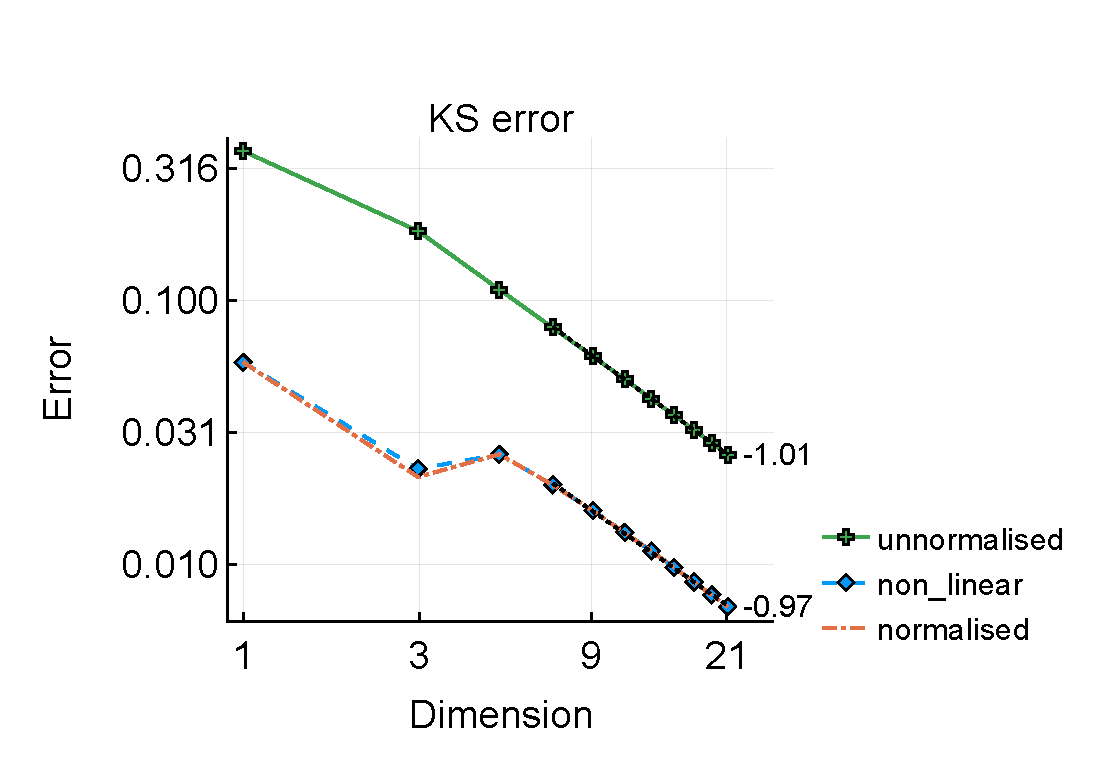
\includegraphics[width=0.5\textwidth,trim={0.5cm 0.8cm 0.2cm 1.25cm},clip]{chapter6/figs/qbdrap_closing_vec/fun4/ks_error_formatted.pdf}%
		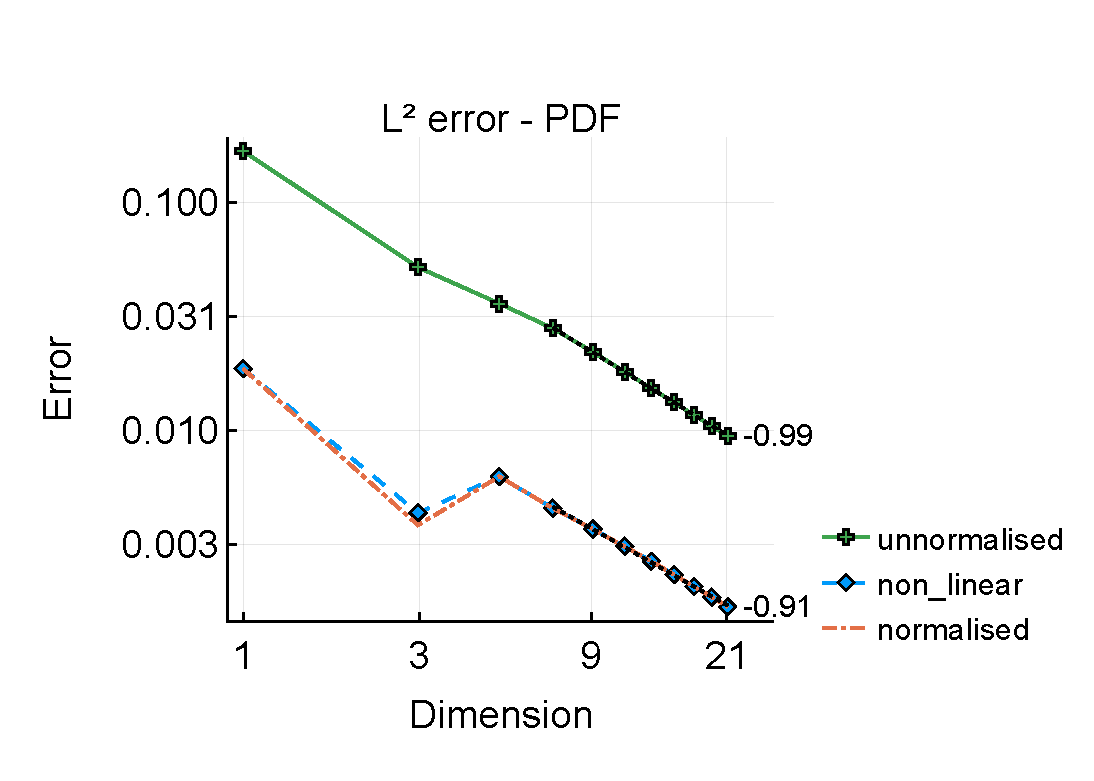
\includegraphics[width=0.5\textwidth,trim={0.5cm 0.8cm 0.2cm 1.25cm},clip]{chapter6/figs/qbdrap_closing_vec/fun4/l2_pdf_error_formatted.pdf}
		\caption{KS error (left) and \(L^2\) error of the PDF (right) of Example~\ref{ex: al} for the three closing vectors considered; unnormalised (green solid line), non-linear normalised (blue dashed line) and normalised (orange dash-dotted line). The error curves of the error curves of the non-linear normalised and normalised closing vectors are almost coincident. The black dotted lines are linear least-squares fits to the last 8 data points and the slopes of the least square lines are written next to the last point.}
		\label{fig: fun 4 ks error qbdrap closing vecs}
	\end{figure}
	Now consider approximating the initial density \(f(x)=1\) for \(x\in[0,1)\). Observing Figure~\ref{fig: fun 4 ks error qbdrap closing vecs} of the KS error and \(L^2\) error of the PDF we now see that the normalised reconstructions outperform the unnormalised reconstruction. This suggests that, in this case, the `folding' of the closing operator about \(\Delta\) has greatly increased the ability of the reconstruction to approximate this initial distribution. 


Some insight is gained by looking at Figure~\ref{fig: pdf reconstructed} where we plot the reconstructed PDFs for the unnormalised (\ref{eqn: alal}) and normalised (\ref{eqn:5462}) closing operators for dimension 1, 3, 5 and 7, as well as the true PDF. Observing Figure~\ref{fig: pdf reconstructed} notice that the unnormalised reconstruction fails to capture the density at the left of each of the plots. This feature is due to a significant amount of mass being lost due to the truncation. In comparison, the reconstruction with the normalised closing operator is much better in this region due to the `folding' around \(\Delta\) in the construction of the closing operator. The `folding' in the normalised closing operator manifests itself as more mass is to the left of these plots compared to the unnormalised reconstructions. % Recall that, as discussed in Section~\ref{}, for the reconstruction we must to allocate the initial condition to a phase with positive rate, or negative rate, so that we can use the appropriate approximation and reconstruction method as discussed in Section~\ref{sec: closing}. Here we suppose that the phase is positive, so the `folding' around \(\Delta\) in the normalised closing operators appears appears at the left of the plots. In general, reconstructions via the unnormalised closing operator typically underestimate the value of the function in this region. 

\begin{figure}[h]
	\centering
	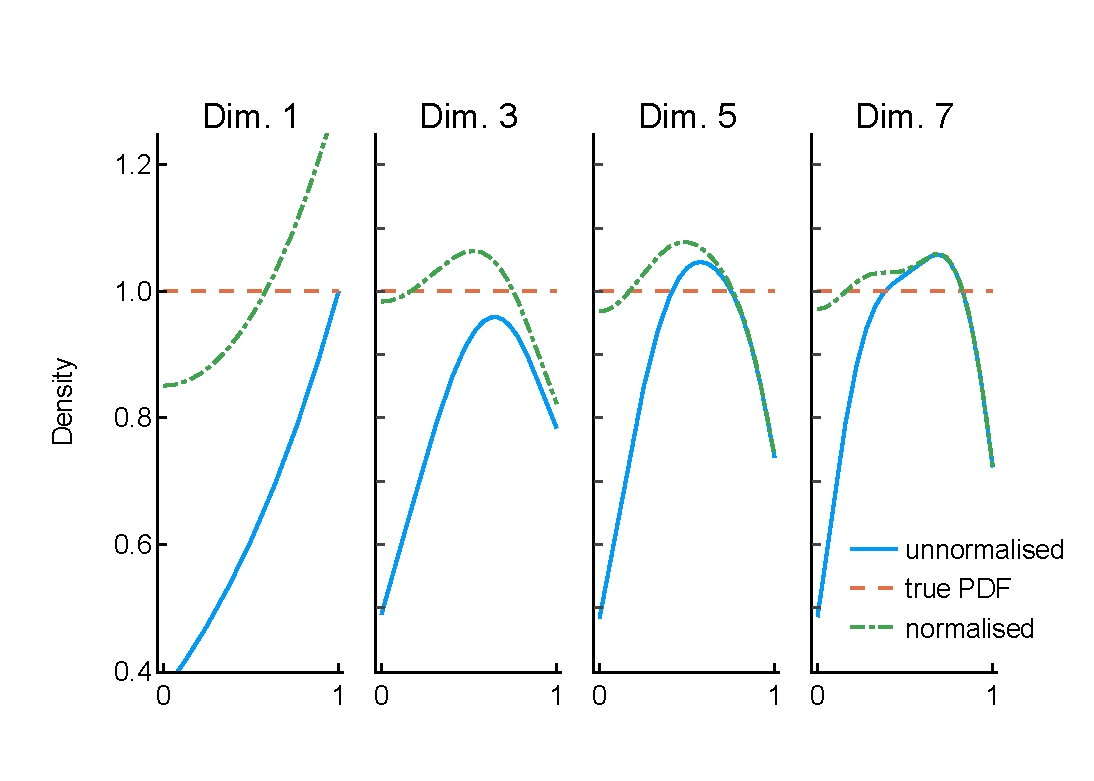
\includegraphics[width=\textwidth,trim={0cm 1.25cm 0cm 1.25cm},clip]{chapter6/figs/qbdrap_closing_vec/fun4/pdfs_formatted.pdf}
	\caption{Approximations to the PDF \(f(x)=1,\, x\in[0,1)\) (blue dashed line) for Example~\ref{ex: al}, constructed using matrix exponential distributions of various dimensions, and using the unnormalised closing operator (green solid line) and normalised closing operator (orange dash-dotted line).}
	\label{fig: pdf reconstructed}
\end{figure} 
%\exampleFloatBarrier
Figure~\ref{fig: pdf reconstructed} also shows that both closing operators fail to approximate the initial condition well at the right-hand side of the interval. A potential area for further research is to determine if there is a different reconstruction method or another closing operator which could alleviate this issue. 
\end{example}

\begin{example}\label{ex: aasmm}
	\begin{figure}[h]
		\centering
		\includegraphics[width=0.5\textwidth,trim={0.5cm 0.8cm 0.2cm 1.25cm},clip]{chapter6/figs/qbdrap_closing_vec/fun6/ks_error_formatted.pdf}%
		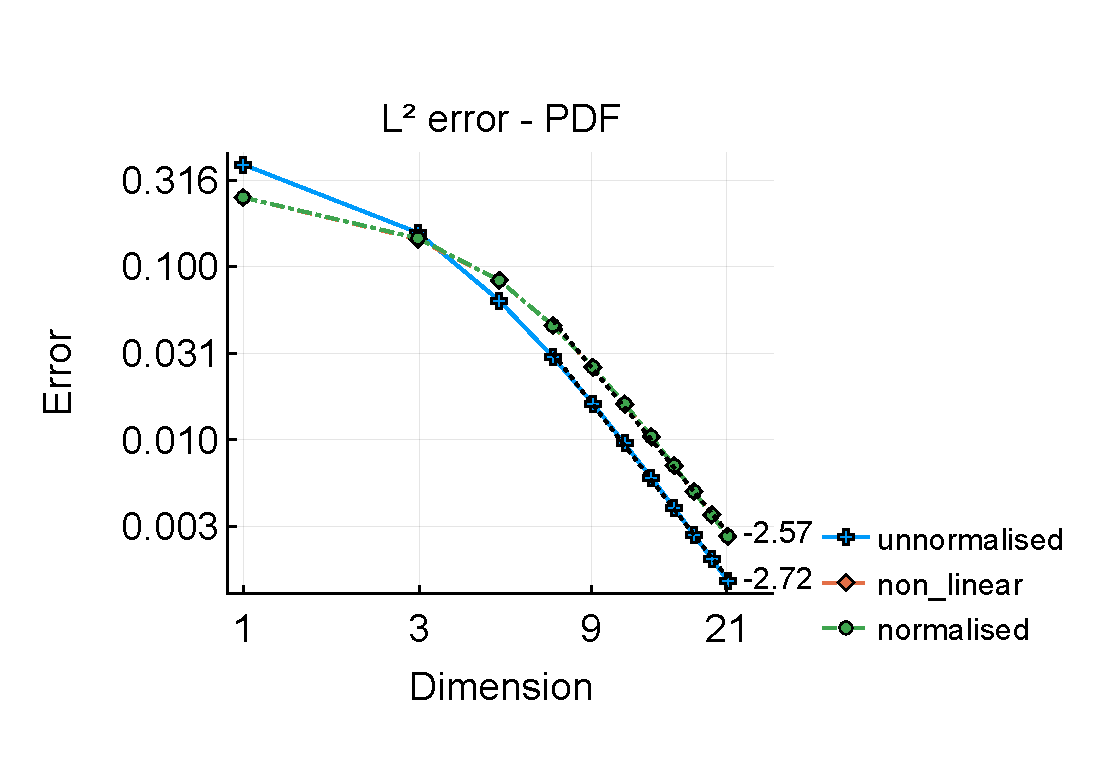
\includegraphics[width=0.5\textwidth,trim={0.5cm 0.8cm 0.2cm 1.25cm},clip]{chapter6/figs/qbdrap_closing_vec/fun6/l2_pdf_error_formatted.pdf}
		\caption{KS error (left) and \(L^2\) error for the PDFs (right) of Example~\ref{ex: aasmm}, for the three closing vectors considered; unnormalised (green solid line), non-linear normalised (blue dashed line) and normalised (orange dash-dotted line). The error curves for the non-linear normalised and normalised closing vectors are almost coincident. The black dotted lines are linear least-squares fits to the last 8 data points and the slopes of the least square lines are written next to the last point.}
		\label{fig: fun 6 ks error qbdrap closing vecs}
	\end{figure}
	Next we consider approximating the initial distribution with density \(-6x^2+6x\) on \([0,1)\). Observing the left-hand panel of Figure~\ref{fig: fun 6 ks error qbdrap closing vecs} which plots the KS error against the dimension of the matrix exponential approximation for the three closing operators, we once again see that the unnormalised closing operator performs the worst, while the performance of the two normalised closing operators is indistinguishable. However, if we instead look at the right-hand panel of Figure~\ref{fig: fun 6 ks error qbdrap closing vecs} which plots the \(L^2\) error between the reconstructed PDF and the true PDF, then the unnormalised closing operator performs better than the two normalised ones for dimension 5 and above. 

	\begin{figure}[h]
		\centering
		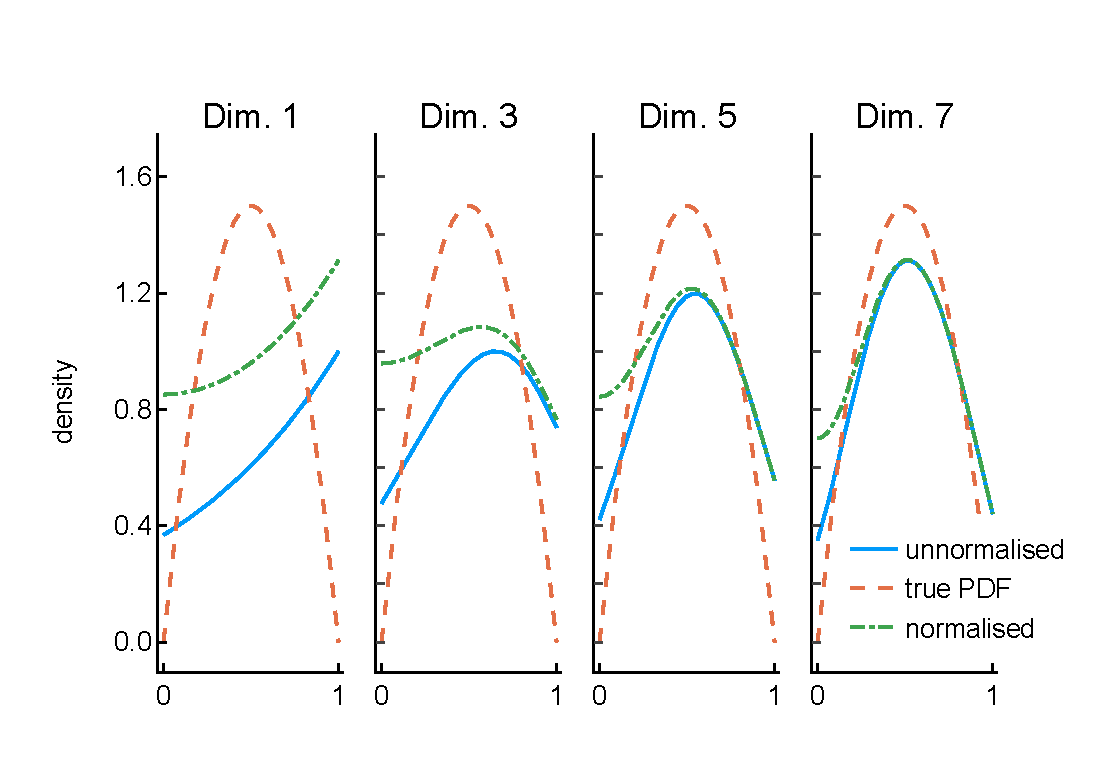
\includegraphics[width=\textwidth,trim={0cm 1.25cm 0cm 1.25cm},clip]{chapter6/figs/qbdrap_closing_vec/fun6/pdfs_formatted.pdf}
		\caption{Approximations to the PDF \(f(x)=-6x^2+6x\) (blue dashed line) for Example~\ref{ex: aasmm}, constructed using matrix exponential distributions of various dimensions, and using the unnormalised closing operator (green solid line) and normalised closing operator (orange dash-dotted line).} 
		\label{fig: pdf reconstructed quadratic}
	\end{figure} 
	%\exampleFloatBarrier
The fact that the unnormalised closing operator outperforms the two normalised ones can be explained by the `folding' of the normalised operators around \(\Delta\). In Figure~\ref{fig: pdf reconstructed quadratic} we plot the reconstructions obtained using the unnormalised and normalised closing operators, along with the true PDF, \(-6x^2+6x\). In Figure~\ref{fig: pdf reconstructed quadratic} at the left of the plots, we observe that the normalised closing operator over-estimate the density function, whereas the unnormalised closing operator looks to be doing better. The `folding' in the normalised closing operator manifests itself as more mass at the left of these plots compared to the unnormalised closing operator. 
\end{example}

\begin{example}\label{ex: kjfk}
	\begin{figure}[h]
		\centering
		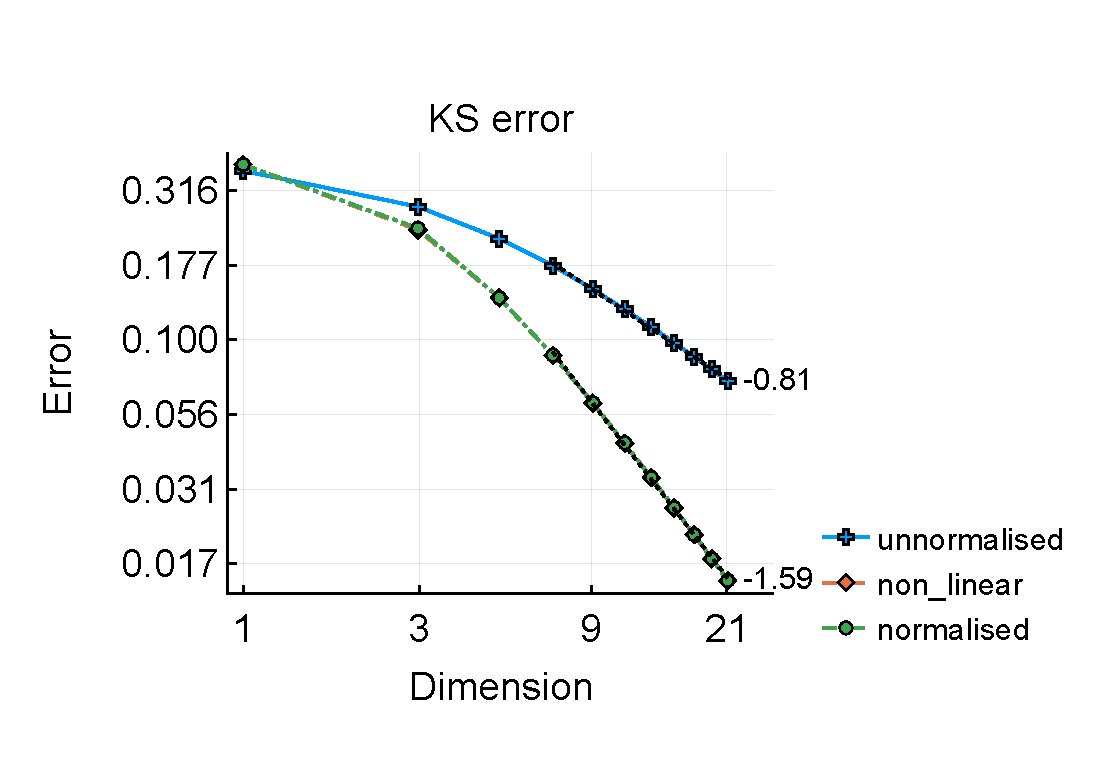
\includegraphics[width=0.5\textwidth,trim={0.5cm 0.8cm 0.2cm 1.25cm},clip]{chapter6/figs/qbdrap_closing_vec/fun7/ks_error_formatted.pdf}%
		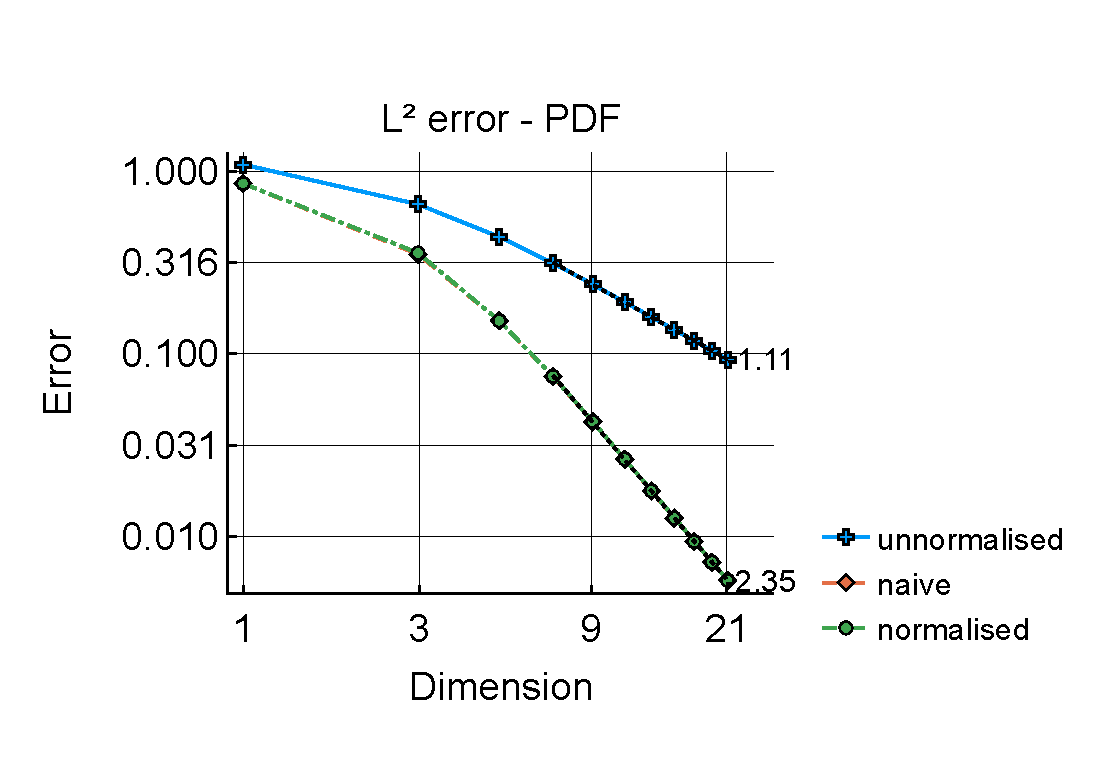
\includegraphics[width=0.5\textwidth,trim={0.5cm 0.8cm 0.2cm 1.25cm},clip]{chapter6/figs/qbdrap_closing_vec/fun7/l2_pdf_error_formatted.pdf}
		\caption{KS error (left) and \(L^2\) error of the PDF (right) for Example~\ref{ex: kjfk} for the three closing vectors considered; unnormalised (green solid line), non-linear normalised (blue dashed line) and normalised (orange dash-dotted line). The error curves for the non-linear normalised and normalised closing vectors are almost coincident. The black dotted lines are linear least-squares fits to the last 8 data points and the slopes of the least square lines are written next to the last point.}
		\label{fig: fun 7 ks error qbdrap closing vecs}
	\end{figure}
	%\exampleFloatBarrier
	Lastly, we consider approximating the initial distribution with PDF \(3e^{-3x}/(1-e^{-3})\). This density function is at a maximum at the left of the region. Considering what we have learnt so far about the unnormalised operator underestimating in this region, we expect that the unnormalised closing operator will perform relatively poorly in this case. Indeed, observing Figures~\ref{fig: fun 7 ks error qbdrap closing vecs} we see that this is the case; the normalised closing operators perform relatively well compared to the unnormalised closing operator, as measured by both error metrics (KS statistic and \(L^2\) norm on the PDF). Plots of the PDFs (omitted), confirm that this is due to the loss of mass at the left-hand side of the region due to the truncation. 
\end{example}

Table~\ref{table: error rates for QBD-RAP closing} summarises the rates of convergence of the \(L^2\) error on the PDFs for unnormalised and normalised closing operators in the examples above (i.e.~the slopes of the black dotted lines in the error plots). In general, the errors of the approximations obtained using normalised closing operators converge at a rate approximately as fast, or faster, than the approximations obtained using the unnormalised closing operator.
\begin{table}
	\centering
	\begin{tabular}{c|c|c|c}
			Example & PDF on \([0,1)\) & \(\beta_1\), unnormalised & \(\beta_1\), normalised \\\hline
			\ref{ex: another example} & \(2\times 1(x<0.5)\) & -1.07 & -0.98 \\
			\ref{ex: al} & 1 & -0.99 & -0.91 \\
			\ref{ex: aasmm} & \(-6x^2+6x\) & -2.72 & -2.57 \\ 
			\ref{ex: kjfk} & \(3e^{-3x}/(1-e^{-3})\) & -1.11 & -2.35 
	\end{tabular}
	\caption{\label{table: error rates for QBD-RAP closing} Estimated rates of convergence, \(\beta_1\), of the \(L^2\) error on the PDFs for unnormalised and normalised closing operators in the examples above (i.e.~the slopes of the black dotted lines in the error plots).}
\end{table} 

In summary, the non-linear normalised and normalised closing operators perform almost identically. In some cases the unnormalised closing operator can outperform the normalised closing operators, typically when the mass of the function to be approximated at the left-hand edge of the cell is low. Further, the rates of convergence for all three schemes were similar to each other, except for in Example~\ref{ex: kjfk} where we approximated the initial condition \(3e^{-3x}/(1-e^{-3})\); in this case the rate of convergence of the normalised closing operators was approximately twice as large as the unnormalised version. Given the results above and its theoretical tractability, we will opt to use the normalised closing operator in (\ref{eqn:5462}) for the rest of the numerical experiments.

\FloatBarrier
\subsection{Comparison of schemes}\label{sec: comp}
Here we compare the ability of the QBD-RAP, uniformisation, and DG schemes to reconstruct initial conditions. With this section we aim to investigate the accuracy of the reconstruction methods for the numerical schemes without any dynamics. 

\begin{example}\label{ex: exa}
	\begin{figure}[h]
		\centering
		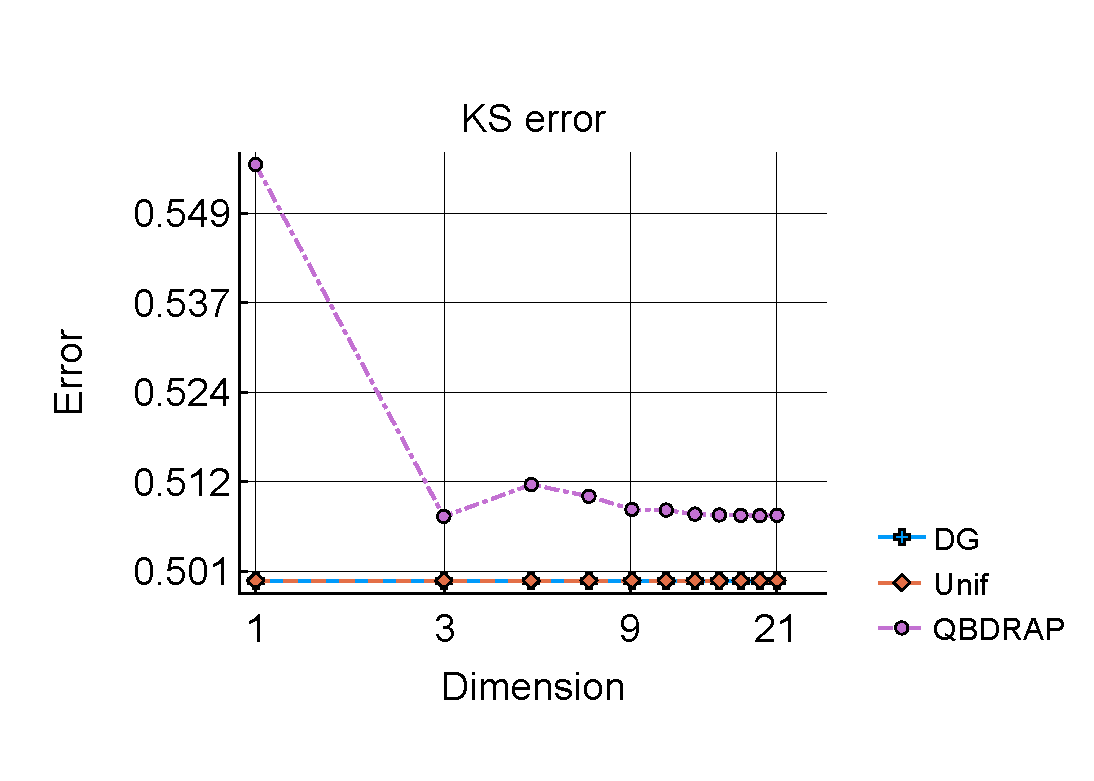
\includegraphics[width=0.5\textwidth,trim={0.5cm 0.8cm 0.2cm 1.25cm},clip]{chapter6/figs/comp/fun1/meshs_ks_error_formatted.pdf}%
		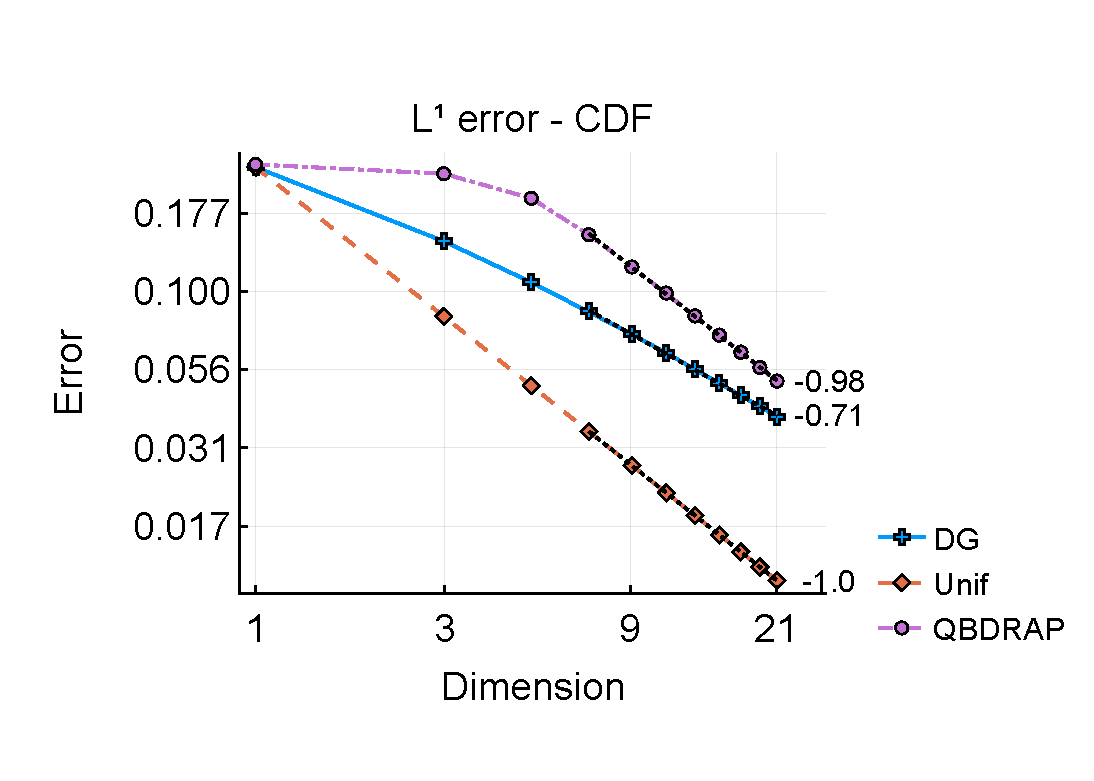
\includegraphics[width=0.5\textwidth,trim={0.5cm 0.8cm 0.2cm 1.25cm},clip]{chapter6/figs/comp/fun1/meshs_l1_cdf_error_formatted.pdf}
		\caption{KS error (left) and \(L^1\) error of the CDF (right) of Example~\ref{ex: exa} for the DG (blue solid line), uniformisation (orange dashed line) and QBD-RAP (purple dashed line) schemes. The black dotted lines are linear least-squares fits to the last 8 data points and the slopes of the least square lines are written next to the last point.}
		\label{fig: fun 1 comp} 
	\end{figure} 
	First we consider the initial condition with CDF \(1(x\geq 0.5)\), that is, a point mass of \(1\) at \(0.5\). This distribution does not have a PDF, so we compare the CDFs only. In Figure~\ref{fig: fun 1 comp} we plot the KS metric (left) and \(L^1\) metric (right) between the true CDF and the reconstructed approximations. Observing the KS metric, it appears that none of the schemes converge and the KS error sits around 0.5 for all schemes. This reflects the fact that convergence in distribution implies point-wise convergence of the CDFs except, perhaps, at points of discontinuity. None of the schemes converge at the discontinuity at \(x=0.5\). Observing the \(L^1\) error between the true CDF and reconstructed approximation (which is the area between the two CDFs) we now see that the schemes appear to show the convergent behaviour we expect. Here, for dimensions up to 21, the uniformisation scheme appears to perform the best, while the QBD-RAP scheme performs the worst, however the QBD-RAP approximation appears to be converging at a faster rate and may outperform the DG approximation if a higher dimension is used.

Perhaps it is no surprise that the uniformisation scheme performs best. In the uniformisation scheme, as we increase the dimension, we partition the cell \([0,1)\) into smaller sub-cells, and use constant functions on each sub-cell to construct an approximate initial density. As such, the uniformisation scheme can produce a piecewise continuous, linear approximation to the CDF. In contrast, both the DG and QBD-RAP schemes result in a smooth approximation to the CDF over the entire cell. Given the initial distribution is far from smooth (it is a point mass), then we might expect that the uniformisation scheme will perform relatively well. 

\begin{figure}[h]
	\centering
	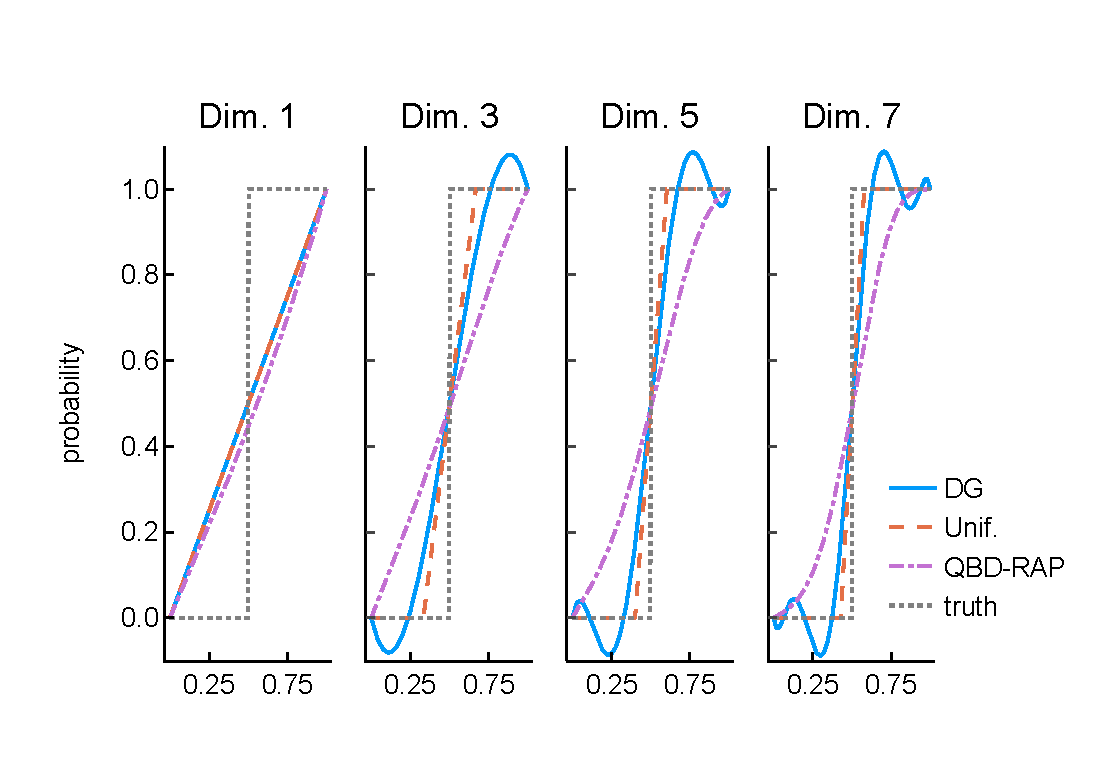
\includegraphics[width=\textwidth,trim={0cm 1.25cm 0cm 1.25cm},clip]{chapter6/figs/comp/fun1/cdfs_formatted.pdf}
	\caption{Reconstructed CDFs using the DG (blue solid line), uniformisation (orange dashed line) and QBD-RAP (purple dashed line) schemes for Example~\ref{ex: exa}. The true distribution function is \(1(x\geq 0.5)\) (grey dotted line).}
	\label{fig: pdf comp fun 1}
\end{figure} 
%\exampleFloatBarrier
In Figure~\ref{fig: pdf comp fun 1} we plot approximate CDFs from the DG, uniformisation and QBD-RAP schemes alongside the true CDF. The DG scheme displays undesirable features for an approximation to a CDF -- it is not monotonically increasing and is not constrained to the bounds of probability, \([0,1]\). On the other hand, although the QBD-RAP scheme converges slowest, it displays good properties in that it results in a monotonically increasing CDF, starting at 0 and ending at 1. The uniformisation scheme approximates the CDF exceptionally well.
\end{example}

\begin{example}\label{eqn: example something}
	\begin{figure}[h]
		\centering
		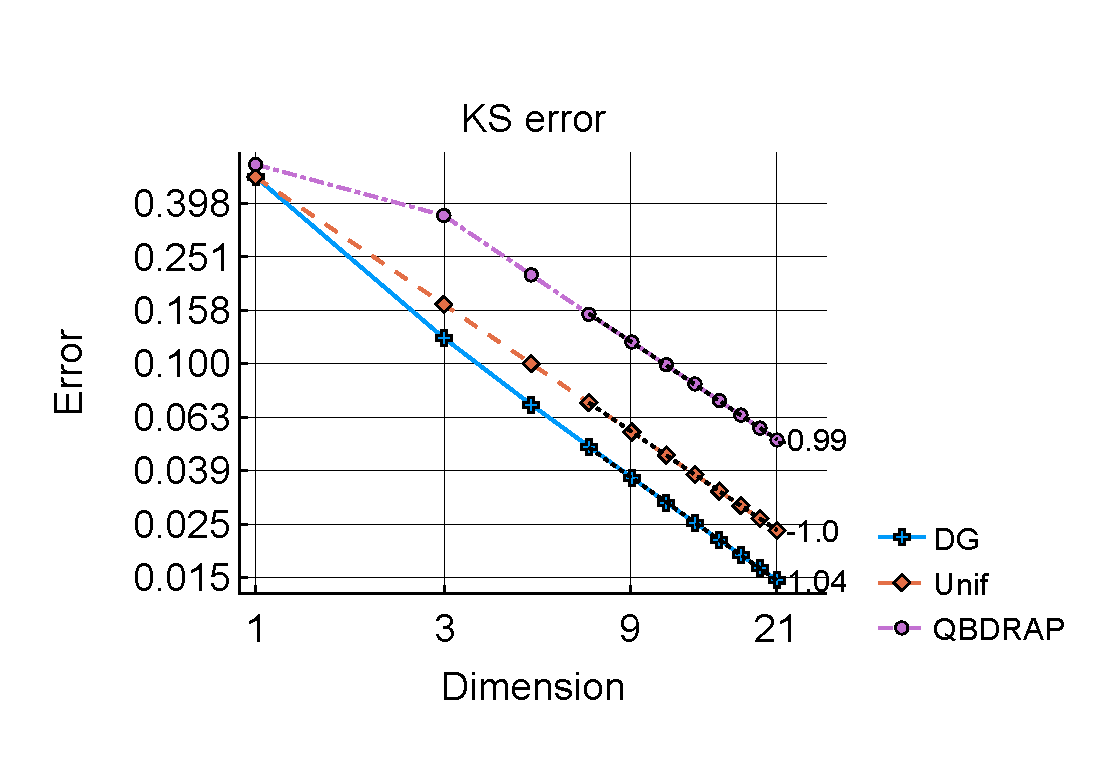
\includegraphics[width=0.5\textwidth,trim={0.5cm 0.8cm 0.2cm 1.25cm},clip]{chapter6/figs/comp/fun2/meshs_ks_error_formatted.pdf}%
		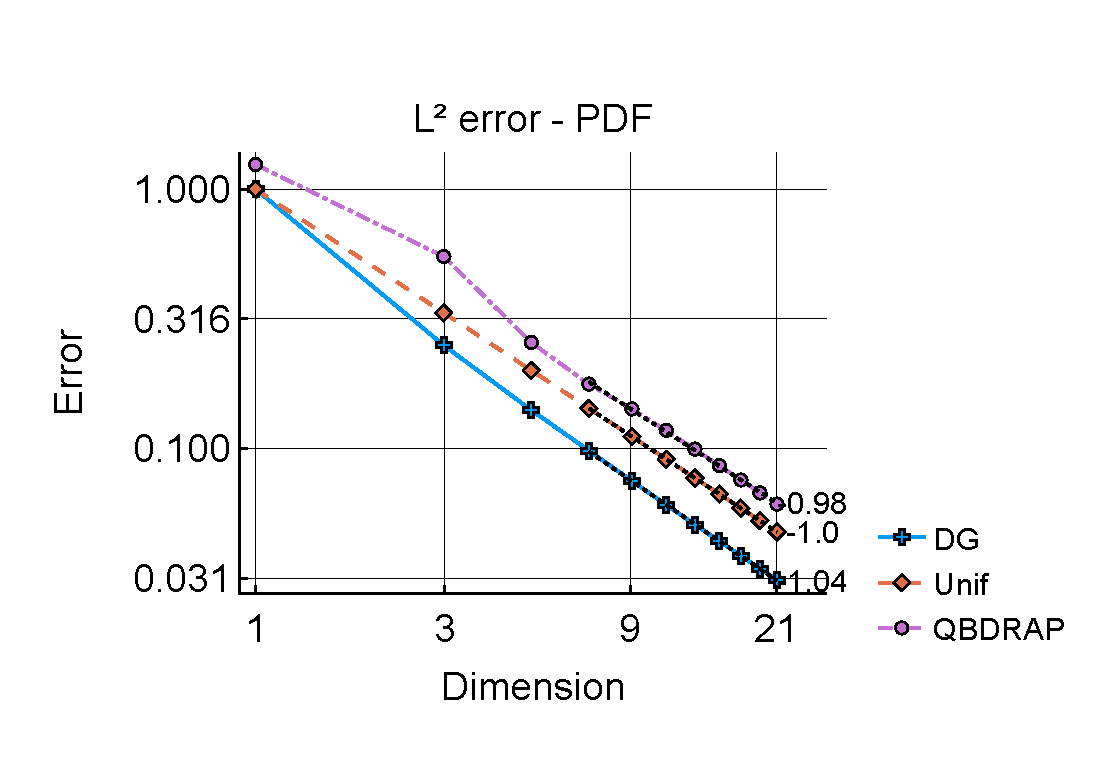
\includegraphics[width=0.5\textwidth,trim={0.5cm 0.8cm 0.2cm 1.25cm},clip]{chapter6/figs/comp/fun2/meshs_l2_pdf_error_formatted.pdf}
		\caption{KS error (left) and \(L^2\) error of the PDF (right) for Example~\ref{eqn: example something} for the DG (blue solid line), uniformisation (orange dashed line) and QBD-RAP (purple dashed line) schemes. The black dotted lines are linear least-squares fits to the last 8 data points and the slopes of the least square lines are written next to the last point.}
		\label{fig: fun 2 comp} 
	\end{figure}
	%\exampleFloatBarrier
	Now consider approximating the initial distribution with PDF \(2\times 1(x\leq 0.5)\). Figure~\ref{fig: fun 2 comp} plots the KS error (left) and \(L^2\) error between the true and approximate PDFs (right). Figure~\ref{fig: fun 2 comp} suggests that all schemes converge at a similar rate for this problem. Here, the QBD-RAP scheme performs worst, the uniformisation scheme second, and the DG scheme the best. However, once again the DG scheme exhibits undesirable properties (plots not shown) -- the approximation to the CDF is at some points above 1 and is not monotonic (although these violations do not appear to be as severe in this case as they were for Example~\ref{ex: exa}). 
\end{example}

\begin{example}\label{ex: alllll}
	\begin{figure}[h]
		\centering
		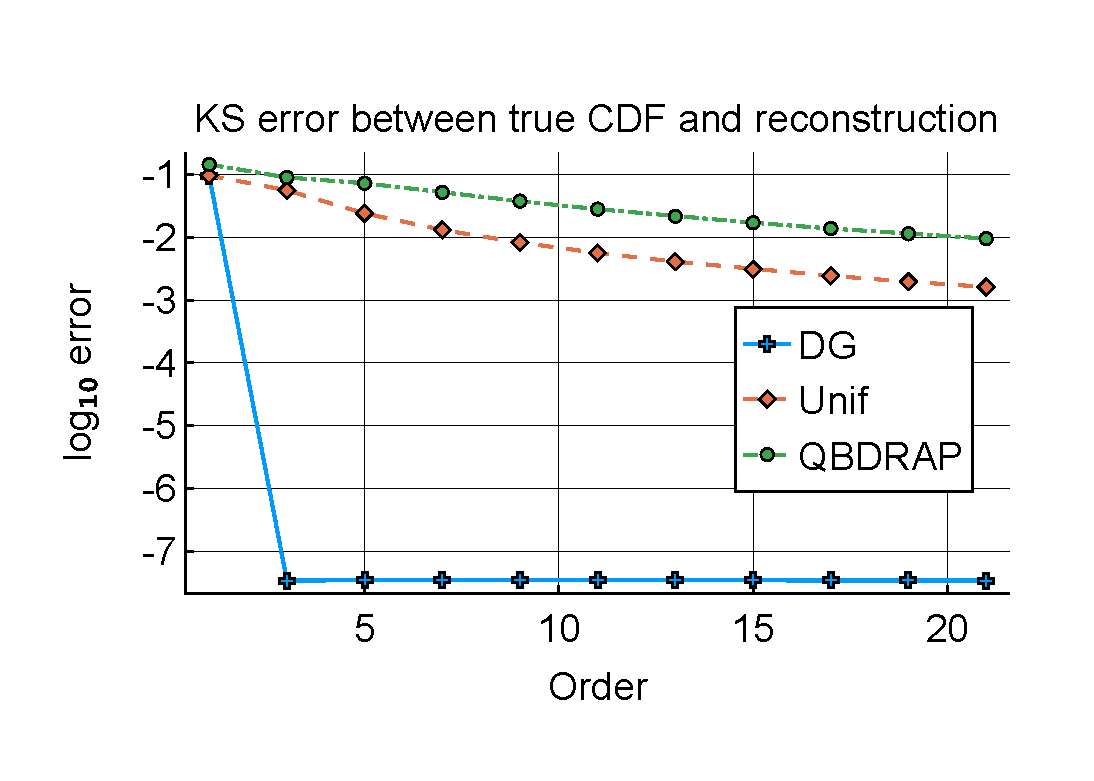
\includegraphics[width=0.5\textwidth,trim={0.5cm 0.8cm 0.2cm 1.25cm},clip]{chapter6/figs/comp/fun6/meshs_ks_error_formatted.pdf}%
		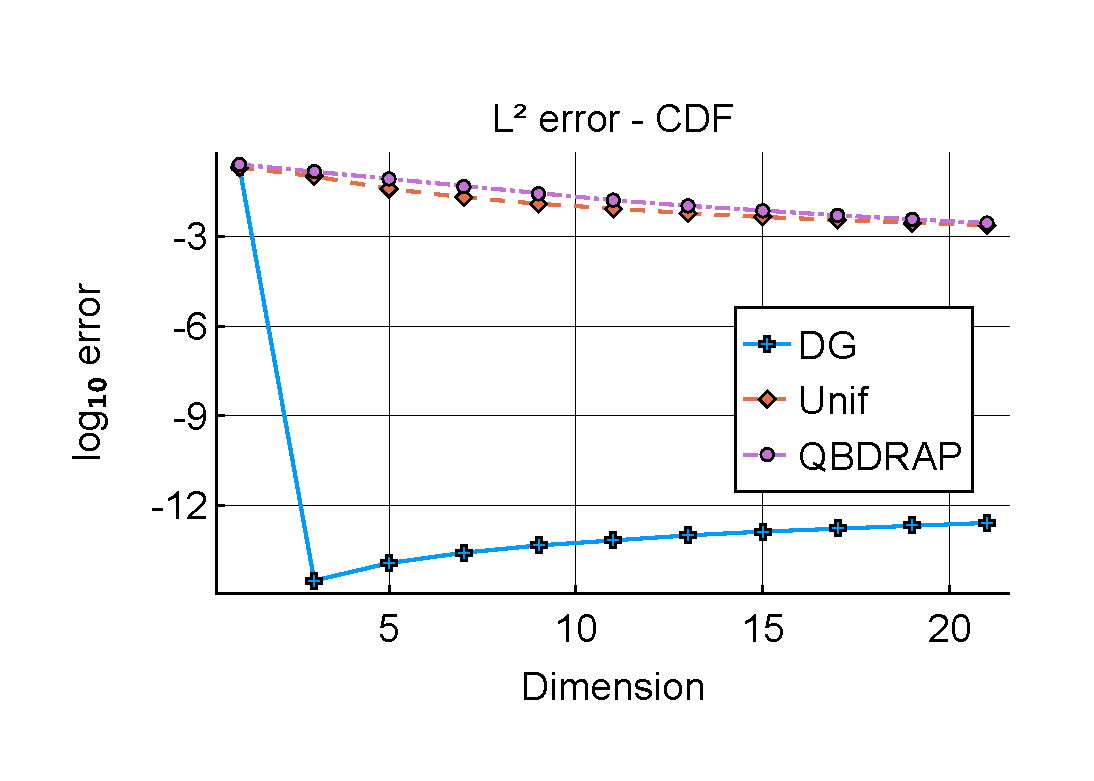
\includegraphics[width=0.5\textwidth,trim={0.5cm 0.8cm 0.2cm 1.25cm},clip]{chapter6/figs/comp/fun6/meshs_l2_pdf_error_formatted.pdf}
		\caption{KS error (left) and \(L^2\) error of the PDF (right) for Example~\ref{ex: alllll} for the DG (blue solid line), uniformisation (orange dashed line) and QBD-RAP (purple dashed line) schemes. The black dotted lines are linear least-squares fits to the last 8 data points and the slopes of the least square lines are written next to the last point.}
		\label{fig: fun 6 comp} 
	\end{figure}
	%\exampleFloatBarrier
	So far we have considered two problems which exhibit discontinuities. At the other extreme we now consider an initial distribution with density \(-6x^2+6x\) on \([0,1)\). In Figure~\ref{fig: fun 6 comp} we plot the KS error and the \(L^2\) error between the true and approximate PDFs. Since the DG method projects the initial condition onto a polynomial basis, then, for a dimension 3 approximation and above, the DG scheme can represent the initial condition exactly. This is reflected in Figure~\ref{fig: fun 6 comp}, where the blue curve drops sharply from dimension 1 to 3, then plateaus. Due to numerical integration errors, for example in the evaluation of the integral in the \(L^2\) norm, the errors for the DG scheme are not 0. Regarding the other two schemes, they too appear to be convergent at approximately the same rate, with the uniformisation scheme performing better for the KS error, and both performing similarly in terms of the \(L^2\) error. 
\end{example}

\begin{example}\label{ex: aalllkkdd}
	\begin{figure}[h]
		\centering
		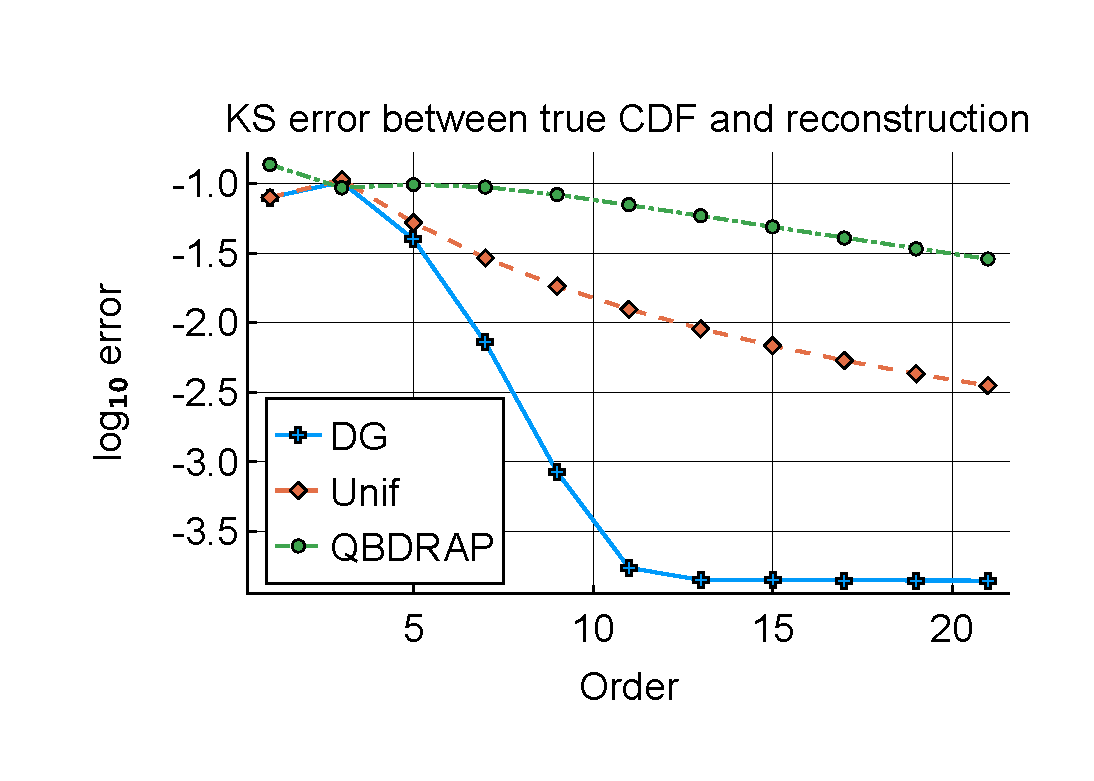
\includegraphics[width=0.5\textwidth,trim={1.1cm 0.8cm 0.1cm 1.25cm},clip]{chapter6/figs/comp/fun9/meshs_ks_error_formatted.pdf}%
		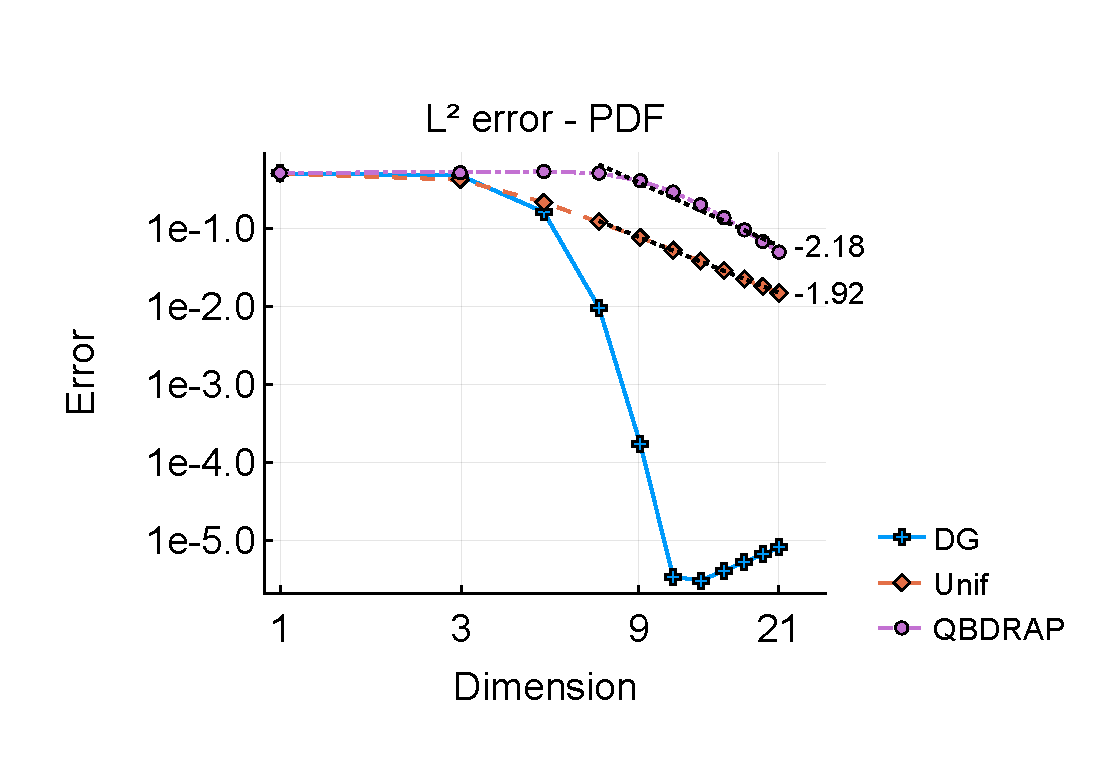
\includegraphics[width=0.5\textwidth,trim={1.1cm 0.8cm 0.1cm 1.25cm},clip]{chapter6/figs/comp/fun9/meshs_l2_pdf_error_formatted.pdf}
		\caption{KS error (left) and \(L^2\) error of the PDF (right) for Example~\ref{ex: aalllkkdd} for the DG scheme (blue solid line), uniformisation scheme (orange dashed line) and QBD-RAP scheme (purple dashed line). The black dotted lines are linear least-squares fits to the last 8 data points and the slopes of the least square lines are written next to the last point.}
		\label{fig: fun 9 comp} 
	\end{figure}
	%\exampleFloatBarrier
	Consider now the initial distribution with PDF \(cos(4\pi(x+0.5))+1\). Figure~\ref{fig: fun 9 comp} shows the KS and \(L^2\) errors for the PDF. Both the KS error (left) and \(L^2\) norm between the true and approximated PDFs (right) tell a similar story; for sufficiently high order, the DG scheme approximates the initial condition very well. The uniformisation scheme performs second best, while the QBD-RAP scheme performs poorest. 
\end{example}

\subsection*{Summary}
First, we investigated the three proposed closing operators for the QBD-RAP scheme proposed in Section~\ref{sec: closing}. We concluded that the normalised closing operator is most appropriate, hence we will use it for the rest of this chapter. 

Next, we investigated reconstructing approximations to initial conditions for the DG, QBD-RAP and uniformisation schemes. We observed that the DG scheme performs well with respect to the error metrics considered, but can display oscillations and result in approximations which violate the axioms of probability. On the other hand, the uniformisation and QBD-RAP schemes result in non-decreasing approximations to the CDFs, but can converge slower with respect to the error metrics considered, with the QBD-RAP scheme often converging the slowest. 

This section investigated the performance of the schemes without considering any of the dynamics of the problem. By doing so, we have gained insights into the performance of the approximations independent of the dynamics. In the remaining sections we introduce dynamics into the problem. %Throughout the remainder of this chapter, keeping the findings of this section in mind will help us understand which errors are due to the reconstruction of the solution, and which errors are due to the approximation of the dynamics of the problem.
\FloatBarrier

\section{Travelling wave problems}\label{sec: wave num}
Here we investigate the performance of the different schemes for approximating transient distributions of one-dimensional travelling wave problems with various initial conditions. Consider a (trivial) fluid queue with one phase, generator \(\bs T=[0]\) and rate \(c=1\). The PDE (if/when it exists) which describes this system is 
\[\cfrac{\partial}{\partial t} f(x,t) = -\cfrac{\partial}{\partial x} f(x,t),\]
where \(f(x,t)\) is the density (if/when it exists) at time \(t\). Given an initial condition, \(f(x,0)\), solutions to this problem are given by 
\[f(x,t) = f(x-t,0)\]
so the solution at time \(t\) is just a shift in the initial condition \(t\) units to the right. We suppose that the fluid queue is bounded, with a lower boundary \(x=0\) and upper boundary \(x=10\). This example is convenient as it has a known solution and no stochastic dynamics, hence we can investigate the ability of the schemes to approximate the flow of mass, without any stochastic dynamics. 

We use the QBD-RAP, uniformisation and DG schemes to discretise the solution in space and discretising the interval \([0,10]\) into \(10\) cells, each of width 1. We use $10,001$ points to approximate the integrals which appear in the construction of the initial conditions, to approximate the integrals appearing in the error metrics, and also as a set of discrete points on which to evaluate the CDFs to approximate the KS metric. Furthermore, we use the SSPRK4 method to integrate over time with a \(t\)-step size of \(0.005\), and we evolve the system until time \(t=4\).\footnote{The \(t\)-step size must be chosen to ensure that numerical integration over time is stable up to dimension 21, adhering to a CFL-like condition \cite[Section~4.8]{nodalDGBook}.} For the DG scheme we also implement the Generalised MUSCL slope limiter in the form of the DG-lim and DG-lin-lim schemes (see also Section~\ref{sec: slope limiting}). 

To investigate the performance of the schemes without the need to reconstruct the function within each cell we use the cell-wise error metric obtained by computing 
\begin{align}
	&\sum_{\ell=1}^{10} \left|\mathbb P(X(4)\in\calD_{\ell,1}, \varphi(4)=1\mid X(0)=0.5,\varphi(0)=1)-p(4,\ell,1)\right|\nonumber 
	\\&+\left|\mathbb P(X(4)\in\{10\}, \varphi(4)=1\mid X(0)=0.5,\varphi(0)=1)-p(4,11,1)\right| \label{eqn: cell errors}
\end{align}
where 
\begin{align}
	\mathbb P(X(4)\in\{10\}, \varphi(4)=1\mid X(0)=0.5,\varphi(0)=1) \label{eqn: cell probs boundary}
\end{align}
is the mass at the boundary, \(p(4,\ell,1)\) is an approximation to \(\mathbb P(X(4)\in\calD_{\ell,1}, \varphi(4)=1\mid X(0)=0.5,\varphi(0)=1)\), and \(p(4,11,1)\) is an approximation to \(\mathbb P(X(4)\in\{10\}, \varphi(4)=1\mid X(0)=0.5,\varphi(0)=1)\).

\begin{example}\label{ex: wave 4}
	\begin{figure}[h]
		\centering
		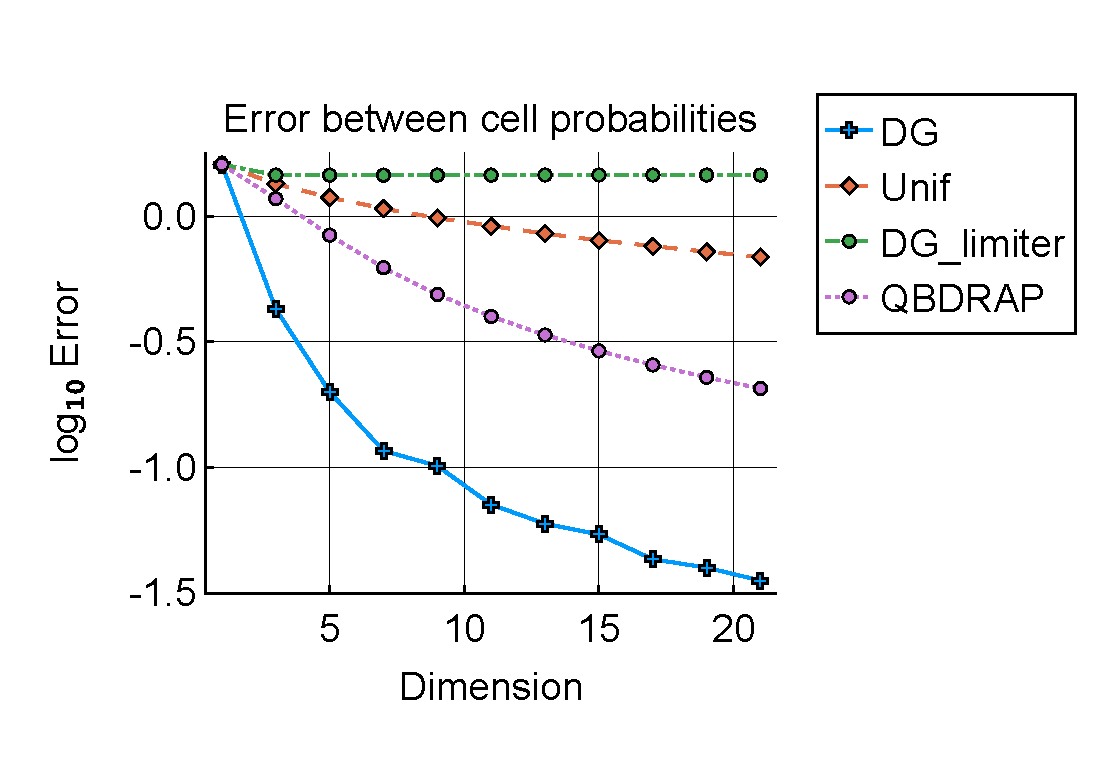
\includegraphics[width=0.5\textwidth,trim={0.75cm 0.8cm 0.25cm 1.25cm},clip]{chapter6/figs/wave/fun4/L1_cell_probs.pdf}
		\caption{Cell-wise error defined in (\ref{eqn: cell errors}) for the travelling wave in Example~\ref{ex: wave 4}. Plotted are the cell-wise errors for the DG (blue solid line), DG-lim scheme (green dashed line), uniformisation (orange dashed line), QBD-RAP (purple dotted line) and DG-lin-lim scheme (gold dashed line) schemes, versus the dimension of the approximation. The black dotted lines are linear least-squares fits to the last 8 data points and the slopes of the least square lines are written next to the last point.}
		\label{fig: fun 4 wave cp} 
	\end{figure}
First consider the initial condition with PDF \(1(x<1)\), a uniform distribution over \((0,1)\). The level of the fluid queue is uniformly distributed over the first cell. For the DG-based schemes (including the uniformisation scheme) the initial condition can be represented exactly whereas, for the QBD-RAP scheme, it cannot. Thus, in this case, there is no discretisation error in constructing the initial condition for the DG and uniformisation schemes. Moreover, at time \(t=4\), the solution is \(f(x,4)=1(x\in[4,5))\). The projections related to the DG-based schemes can represent this solution exactly too, hence we might expect these schemes to work well here. 

We plot the cell-wise error metric in Figure~\ref{fig: fun 4 wave cp} and observe that the DG scheme clearly produces the lowest errors, followed by the QBD-RAP and DG-lin-lim schemes which perform comparably, then the uniformisation scheme. The worst performer is the DG-lim scheme which does not appear to converge; during the integration of the solution over time the DG-lim scheme has detected oscillations and reduced the scheme to linear where the oscillations were detected, thereby decreasing the accuracy of the scheme to linear where oscillations are present. 

\begin{figure}[h]
	\centering
	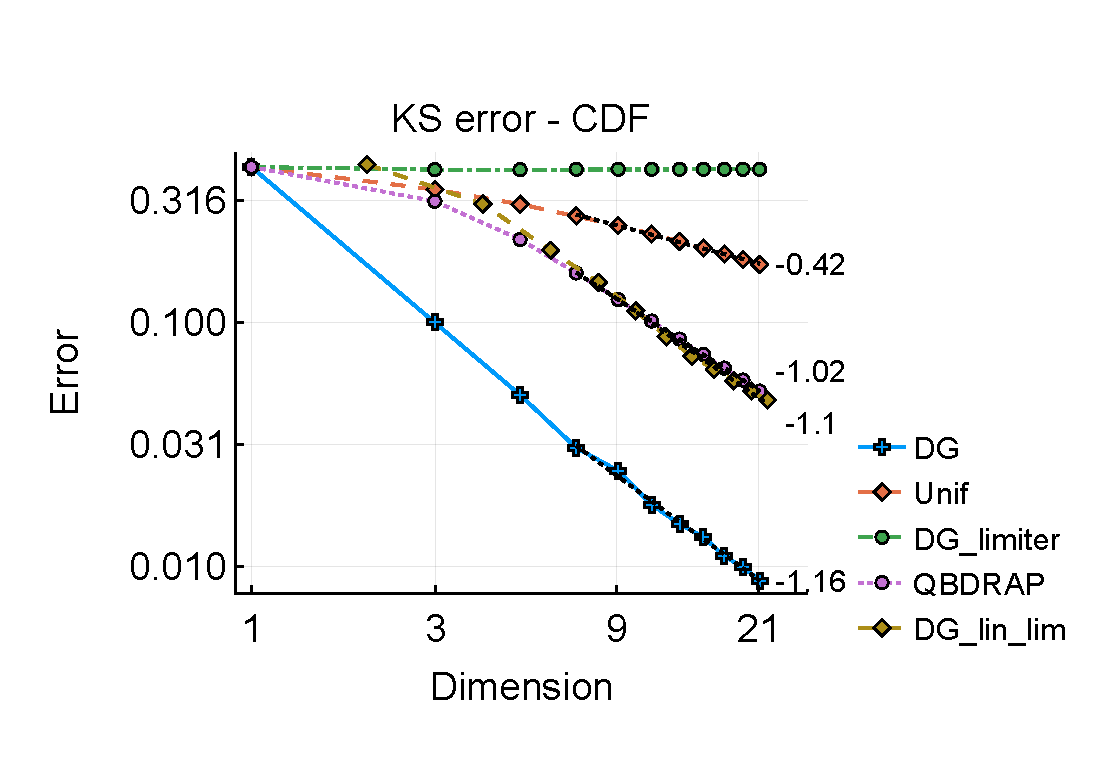
\includegraphics[width=0.5\textwidth,trim={0.75cm 0.8cm 0.25cm 1.25cm},clip]{chapter6/figs/wave/fun4/meshs_ks_error_formatted.pdf}%
	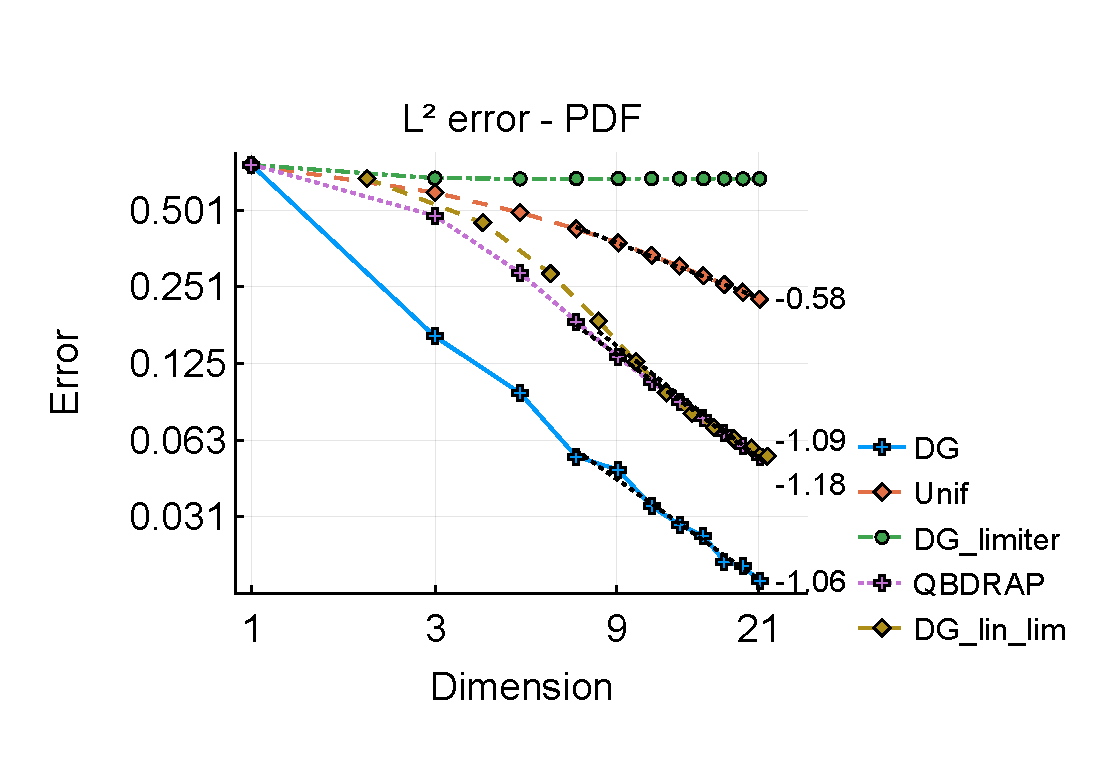
\includegraphics[width=0.5\textwidth,trim={0.75cm 0.8cm 0.25cm 1.25cm},clip]{chapter6/figs/wave/fun4/meshs_l2_pdf_error_formatted.pdf}
	\caption{KS error (left) and \(L^2\) error of the PDF (right) for the travelling wave problem in Example~\ref{ex: wave 4} using the approximations from the DG (blue solid line), DG-lim scheme (green dash-dotted line), uniformisation (orange dashed line), QBD-RAP (purple dotted line) and DG-lin-lim (gold dashed line) schemes. The black dotted lines are linear least-squares fits to the last 8 data points and the slopes of the least square lines are written next to the last point.} 
	\label{fig: fun 4 wave} 
\end{figure}
Figure~\ref{fig: fun 4 wave} plots the KS error between the approximate and true CDFs and \(L^2\) error between the approximate and true PDFs. Comparing Figure~\ref{fig: fun 4 wave cp} with Figure~\ref{fig: fun 4 wave}, each scheme seems to show a similar rate of decay for these two error metrics as they did for the cell-wise errors. 

\begin{figure}[h]
	\centering
	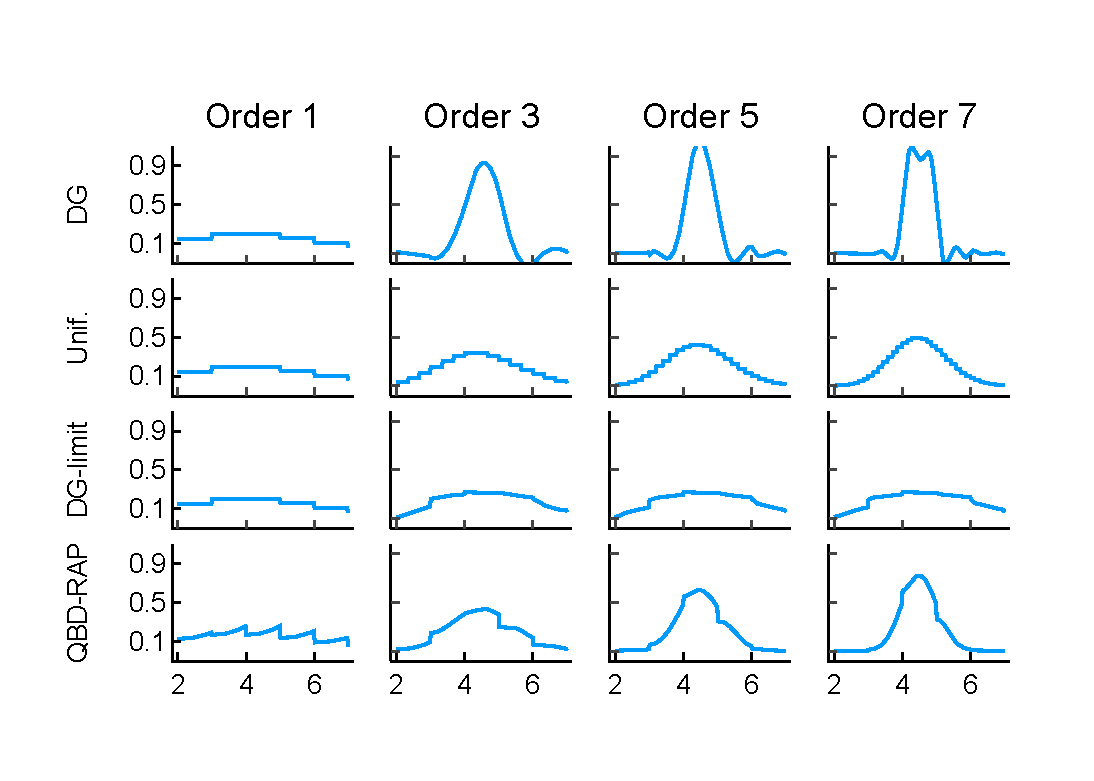
\includegraphics[width=\textwidth,trim={0cm 1.25cm 0cm 1.25cm},clip]{chapter6/figs/wave/fun4/pdfs_formatted.pdf}
	\caption{Reconstructed PDFs using the DG (top row), uniformisation (second row), DG-lim (third row), QBD-RAP (fourth row) and DG-lin-lim schemes (fifth row), for dimension 1, 3, 5, and 7 (columns) for the travelling wave problem in Example~\ref{ex: wave 4}. The true density function is \(1(4\leq x<5)\).}
	\label{fig: pdf wave fun 4} 
\end{figure}
Continuing with Figure~\ref{fig: fun 4 wave}. The DG-lim scheme does not appear to converge with these error metrics. Of the other three positivity preserving schemes, the uniformisation, DG-lin-lim and QBD-RAP schemes, all appear to be converging with the QBD-RAP and  DG-lin-lim schemes converging similarly and faster than the uniformisation scheme. With these error metrics, the DG scheme is converging fastest. However, if we observe the approximations resulting from the DG scheme (Figure~\ref{fig: pdf wave fun 4} top-row), we find them to be unsatisfactory due to oscillations and negative densities. 

Figure~\ref{fig: pdf wave fun 4} plots the density functions reconstructed using the DG, uniformisation, DG-lim, QBD-RAP and DG-lin-lim schemes for various dimension schemes. In the first row observe that, when the dimension is greater than one, the DG scheme (sans limiter) produces an approximation to the PDF which is negative in some places. In the third row of Figure~\ref{fig: pdf wave fun 4} observe that, with the limiter, the DG-lim approximation does not change significantly after dimension 3. This is due to the fact that the DG-lim scheme is at best linear in the presence of oscillations. In the second row of Figure~\ref{fig: pdf wave fun 4} is the solution approximated using the uniformisation scheme, in the fourth row is the solution approximated using the QBD-RAP scheme, and in the last row is the approximation from the DG-lin-lim scheme.

This is a particularly interesting example. For the DG scheme, even though there is no discretisation error for the initial condition, we use a strong stability preserving time-integration method, and the projection on which the DG method is based can represent the transient distribution at time \(t=4\) exactly, there is still the possibility of badly behaved solutions as shown in the top row of Figure~\ref{fig: pdf wave fun 4}.
%\exampleFloatBarrier
\end{example}

\begin{example}\label{ex: wave 2}
Another interesting example occurs with the initial condition with CDF \(1(x\geq 0.5)\), i.e.~a point mass of 1 at \(0.5\). The exact solution at time \(t=4\) is therefore a point mass at \(4.5\). No PDF exists for the true distribution, so instead we compare the CDFs. Also recall that, when we analysed reconstruction of this initial condition we saw that using the KS metric may be uninformative due to the lack of point-wise convergence at the discontinuity, so for this example, we measure errors by looking at the \(L^1\) error between the CDFs (the area between the CDFs) instead, and also with the cell-wise error from (\ref{eqn: cell errors})-(\ref{eqn: cell probs boundary}).

\begin{figure}[h]
	\centering
	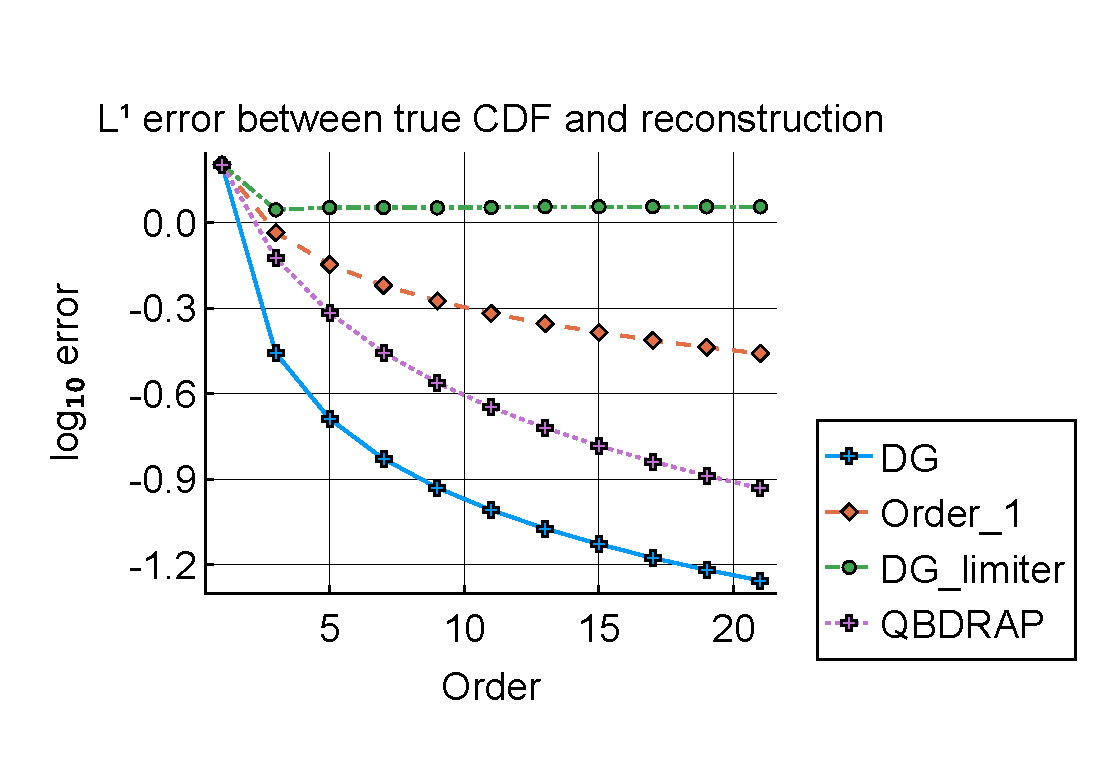
\includegraphics[width=0.5\textwidth,trim={0.75cm 0.8cm 0.25cm 1.25cm},clip]{chapter6/figs/wave/fun2/meshs_l1_cdf_error_formatted.pdf}%
	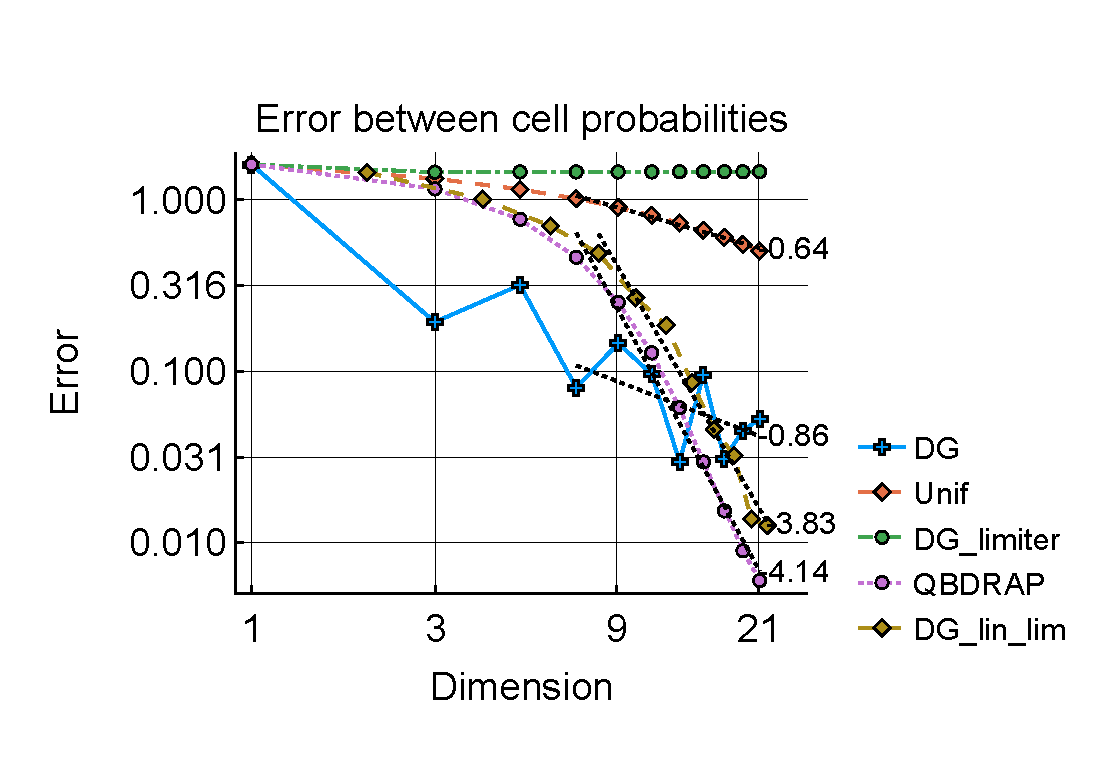
\includegraphics[width=0.5\textwidth,trim={0.75cm 0.8cm 0.25cm 1.25cm},clip]{chapter6/figs/wave/fun2/L1_cell_probs.pdf} 
	\caption{\(L^1\) error of CDFs (left) and the cell-wise error metric in (\ref{eqn: cell errors})-(\ref{eqn: cell probs boundary}) (right) for the travelling wave problem in Example~\ref{ex: wave 2} where approximation were constructed via the DG (blue solid line), DG-lin-lim (green dash-dotted line), uniformisation (orange dashed line), QBD-RAP (purple dotted line) and DG-lin-lim (gold dashed line) schemes. The black dotted lines are linear least-squares fits to the last 8 data points and the slopes of the least square lines are written next to the last point.} 
	\label{fig: fun 2 wave} 
\end{figure}
%\exampleFloatBarrier
Figure~\ref{fig: fun 2 wave} (left) plots the \(L^1\) error between the true and approximated CDFs. The \(L^1\) metric tells a similar story to the previous analysis: the DG-lim scheme does not perform well, the other three positivity preserving schemes (the uniformisation, DG-lin-lim and QBD-RAP schemes) appear to converge, with the QBD-RAP and DG-lin-lim schemes performing similarly and better than the uniformisation scheme. The DG scheme performs the best. However, if we plot the approximations to the CDFs from the DG scheme (not shown) we once again see an oscillating, non-monotonic function. 

Another interesting observation is to compare the performance of the uniformisation and QBD-RAP schemes with respect to the \(L^1\) metric on the CDFs in Figure~\ref{fig: fun 2 wave} (left) to that in Figure~\ref{fig: fun 1 comp} (right). Recall, in Figure~\ref{fig: fun 1 comp} we investigated the ability of the approximation schemes to represent the initial distribution with CDF \(1(x\geq 0.5)\), which is the initial condition of the problem we are considering here. In Figure~\ref{fig: fun 1 comp} (right) the uniformisation scheme out-performed the QBD-RAP scheme at reconstructing the initial condition. However, in Figure~\ref{fig: fun 2 wave} (left) we see that the QBD-RAP scheme out-performs the uniformisation scheme. This suggests that the QBD-RAP scheme is better able to resolve movement of mass across the domain when integrating over time compared to the uniformisation scheme.  

Figure~\ref{fig: fun 2 wave} (right) plots the cell-based error metric in (\ref{eqn: cell errors})-(\ref{eqn: cell probs boundary}). Once again, the DG-lim scheme does not appear to converge. Interestingly, the error curve for the DG scheme is not monotonic which is likely to be caused by the specific location of oscillations in the approximation for different dimension approximations. Furthermore, the DG scheme can result in negative estimates of the cell probabilities in (\ref{eqn: cell errors})-(\ref{eqn: cell probs boundary}) (not shown). Of the other three positivity preserving schemes, the uniformisation, DG-lin-lim and QBD-RAP scheme all appear to converge, with the QBD-RAP and DG-lin-lim schemes performing similarly; even performing better than the DG scheme when the dimension is sufficiently large. The estimated rate of convergence of the QBD-RAP and DG-lin-lim schemes is approximately -4 for this example, which is significantly faster than the rate of convergence of any scheme in any of the other examples in this section (typically around -2 to -1). 
\end{example}

\begin{example}\label{ex: wave 6}
	Now consider an initial distribution which is truncated Gaussian with mean 2.5 and standard deviation 0.5, and truncated at the boundaries, 0 and 10;
	\begin{align}
		\mu([0,x)) = \mathbb P(X(0)\leq x, \varphi(0)=1)=\cfrac{\Phi((x-2.5)/0.5)-\Phi(-2.5/0.5)}{\Phi(7.5/0.5)-\Phi(-2.5/0.5)}, \label{eqn: kdjfksdf}
	\end{align}
	for \(x\in[0,10]\) and where \(\Phi(x)\) is the CDF of the standard normal distribution.

	At time \(t=4\) the distribution is truncated Gaussian with mean 6.5, standard deviation parameter 0.5, and is truncated below at 4.0 and above at 10, and there is also a small mass at the upper boundary; 
	\begin{align}
		\nonumber & \mathbb P(X(4)\leq x, \varphi(4)=1\mid X(0)\sim\mu, \varphi(0)=1)  
		\\=&\cfrac{\Phi((x-4-2.5)/0.5)-\Phi(-2.5/0.5)}{\Phi(7.5/0.5)-\Phi(-2.5/0.5)}1(x\in[4,10)) 
		+ 1(x\geq 10).\label{eqn: bbbbbaabbaa}%\cfrac{\Phi(7.5/0.5)-\Phi(3.5/0.5)}{\Phi(7.5/0.5)-\Phi(-2.5/0.5)}.
	\end{align}
	At time \(t=4\) the mass at the boundary is approximately \(1.28\times 10^{-12}\) and there is also a small discontinuity in the density at \(x=4\).

	\begin{figure}[h]
		\centering
		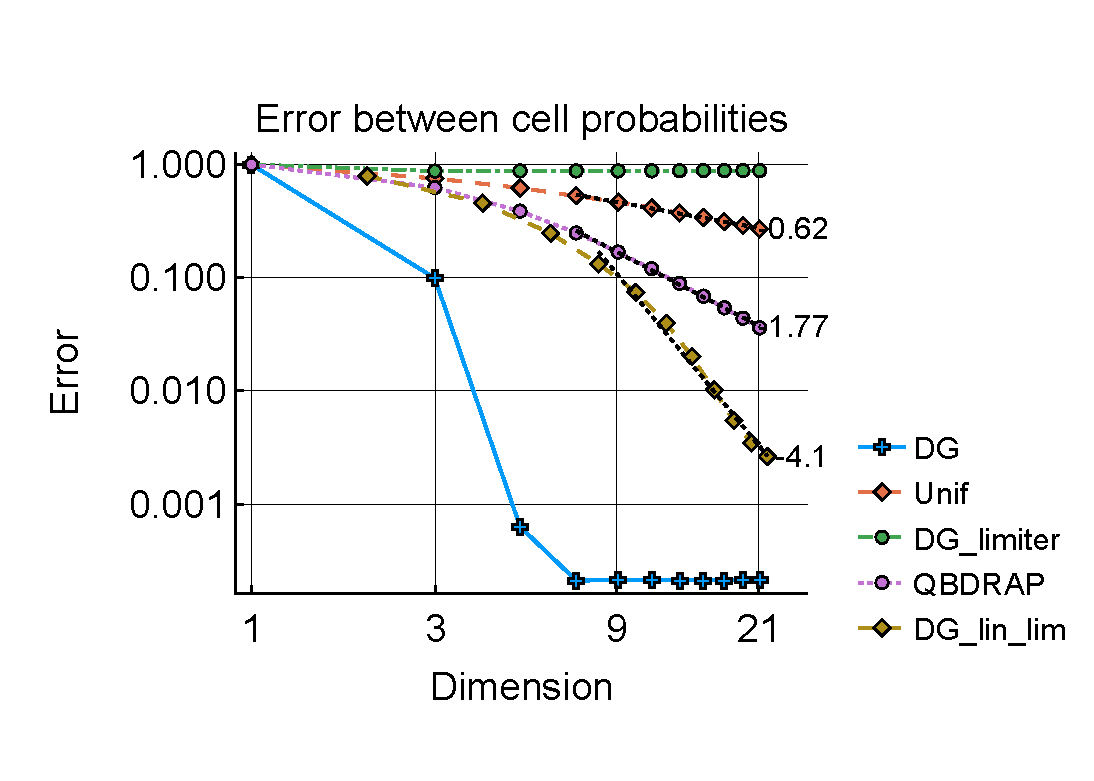
\includegraphics[width=0.5\textwidth,trim={0.75cm 0.8cm 0.25cm 1.25cm},clip]{chapter6/figs/wave/fun6/L1_cell_probs.pdf}
		\caption{Cell-wise error defined in (\ref{eqn: cell errors})-(\ref{eqn: cell probs boundary}) for the travelling wave problem in Example~\ref{ex: wave 6}. Plotted are the cell-wise errors for the DG (blue solid line), DG-lim (green dashed line), uniformisation (orange dashed line), QBD-RAP (purple dotted line) and DG-lin-lim (gold dashed line) schemes, versus the dimension of the approximation. The black dotted lines are linear least-squares fits to the last 8 data points and the slopes of the least square lines are written next to the last point.}  
		\label{fig: fun 6 wave cp} 
	\end{figure}
	Since the magnitude of the discontinuity at \(t=4,\,x=4\) is small (much smaller than numerical integration errors in the evaluation of the error metrics), and the distribution is otherwise smooth, we expect that the DG scheme will perform well for this example. Figures~\ref{fig: fun 6 wave cp} and~\ref{fig: fun 6 wave} confirms that this is indeed the case. For all three error metrics the error obtained by the DG scheme rapidly decreases to a point where it is swamped by other numerical errors. This is characteristic of the DG scheme for the smooth problems we investigate throughout this chapter. For low order DG schemes there are regions where the approximate PDF is negative, however, as the order of the DG scheme increases, these regions disappear. 
	
	Interestingly, even though this is a relatively smooth problem, the DG-lim scheme does not perform well. It must be that the initial and transient distributions are `sufficiently pointy' that oscillations in the numerical solutions occur and the limiter reduces the order of the scheme to linear. 
	
	\begin{figure}[h]
		\centering
		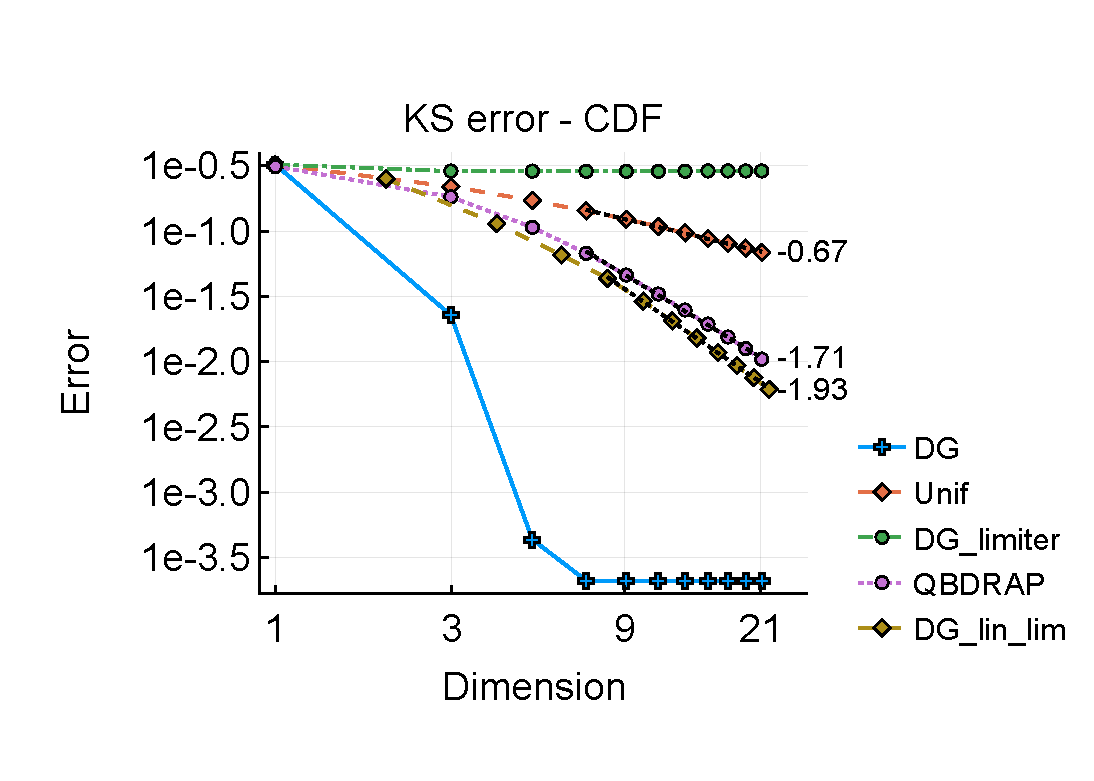
\includegraphics[width=0.5\textwidth,trim={0.75cm 0.8cm 0.25cm 1.25cm},clip]{chapter6/figs/wave/fun6/meshs_ks_error_formatted.pdf}%
		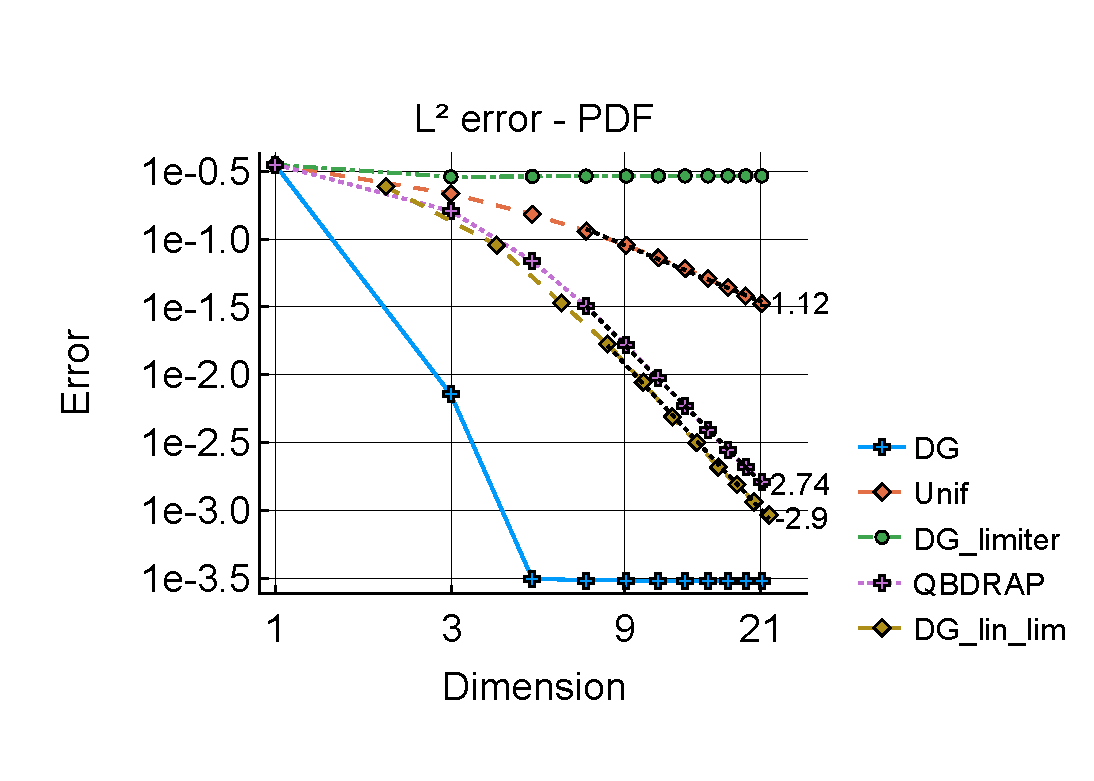
\includegraphics[width=0.5\textwidth,trim={0.75cm 0.8cm 0.25cm 1.25cm},clip]{chapter6/figs/wave/fun6/meshs_l2_pdf_error_formatted.pdf}
		\caption{KS error (left) and \(L^2\) error for the PDFs (right) for Example~\ref{ex: wave 6} where approximations were constructed via the DG (blue solid line), DG-lim (green dash-dotted line), uniformisation (orange dashed line), QBD-RAP (purple dotted line) and DG-lin-lim (gold dashed line) schemes. The black dotted lines are linear least-squares fits to the last 8 data points and the slopes of the least square lines are written next to the last point.} 
		\label{fig: fun 6 wave} 
	\end{figure}
	The other three positivity preserving schemes appear to converge, with the uniformisation scheme performing the worst and the DG-lin-lim scheme performing the best of the three for all error metrics. For the KS and \(L^2\) error on the PDFs in Figure~\ref{fig: fun 6 wave} the DG-lin-lim and QBD-RAP schemes perform similarly, however, for the cell-wise error in Figures~\ref{fig: fun 6 wave cp} the DG-lin-lim scheme performs significantly better than the QBD-RAP scheme. Given that the DG-lin-lim scheme performed similarly to the QBD-RAP scheme for the previous examples, and also for the other error metrics for this example, this is unexpected. 
	
	\begin{figure}[h]
		\centering
		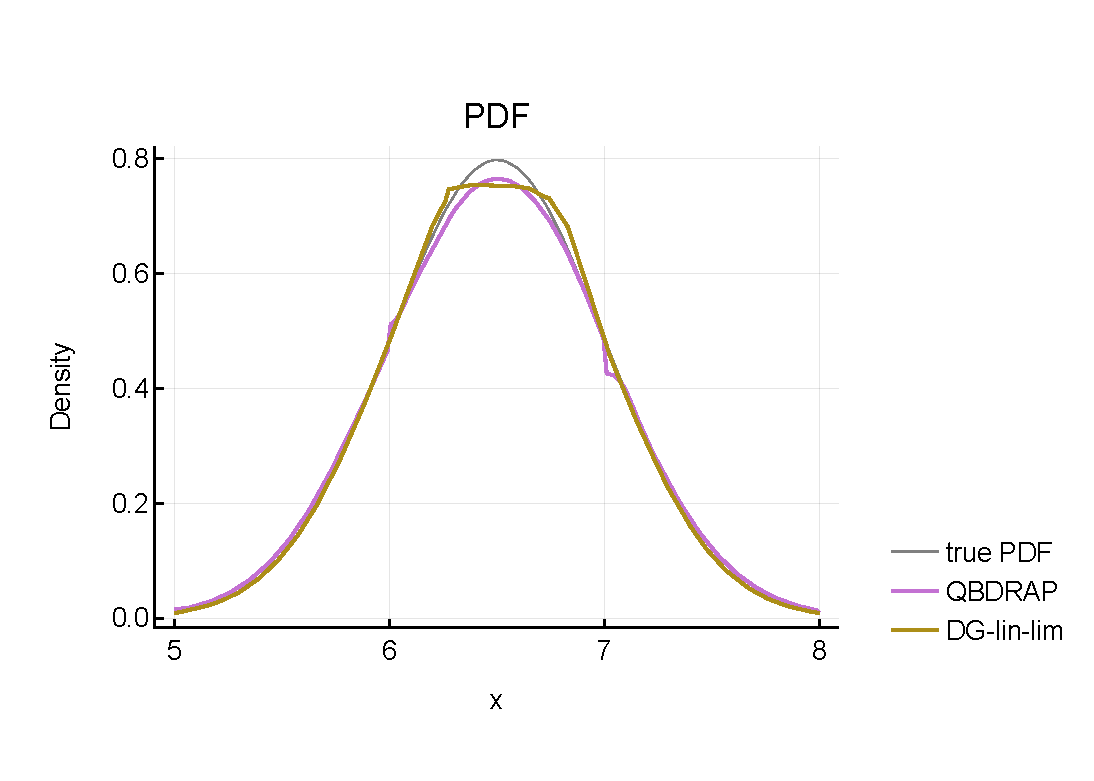
\includegraphics[width=0.8\textwidth,trim={0cm 1.25cm 0cm 1.25cm},clip]{chapter6/figs/wave/fun6/order_21_PDFs_formatted.pdf}
		\caption{Dimension 21 QBD-RAP (purple) and dimension 22 DG-lin-lim (gold) approximations to the transient PDF at time \(t=4\) for Example~\ref{ex: wave 6}. The true PDF is plotted in grey.}  
		\label{fig: fun 6 wave pdfs} 
	\end{figure}
%\exampleFloatBarrier
	To investigate this unexpected fact, in Figure~\ref{fig: fun 6 wave pdfs} we plot the dimension 21 QBD-RAP and dimension 22 DG-lin-lim approximations to the PDF. Figure~\ref{fig: fun 6 wave pdfs} shows that the DG-lin-lim scheme approximates the PDF well, except at the peak located at \(x=6.5\) (the limiter has affected the solution in this region). Specifically, the DG-lin-lim scheme underestimates the density in the peak, but overestimates the density either side of the peak. As a result, when we integrate over \(x\in[6,7]\) to compute the cell-wise probabilities, errors cancel over this region and the DG-lin-lim scheme produces an accurate estimate of the probability in this cell. In comparison, the QBD-RAP scheme also underestimates the density at the peak, but also within the entire interval \([6,7]\), albeit less so at the edges than the middle. The QBD-RAP scheme also overestimates the density in the adjacent cells, \([5,7]\) and \([7,8]\). Hence, the overall cell-wise error is larger for the QBD-RAP scheme.
\end{example}

\begin{example}\label{ex: wave 1}
	We now want to look at how the schemes might handle a mass at the boundary. We introduce an ephemeral second phase into the model with phase transition rate \(T_{22}=-1\), and fluid rate \(c_2=0\). The generator is therefore 
	\[T=\left[\begin{array}{cc} 0 & 0 \\ 1 & -1 \end{array}\right].\]

	We suppose that the initial condition is a point mass of 1 at the boundary \(x=0\) in Phase~\(2\), i.e. \[\mathbb P(X(0)\leq x, \varphi(0)=2)=1(0\leq x).\] 
	With this initial condition, the transient distribution at time \(t=4\) is 
	\begin{align}
		&\mathbb P(X(4)\leq x,\varphi(4)=1 \mid X(0)=0,\varphi(0)=2) \nonumber 
		\\&= \left(e^{T_{22}(4-x)}-e^{T_{22}4}\right)1(4< x) + (1-e^{T_{22}4})1(4\geq x) \nonumber
		\\&= \left(e^{-(4-x)}-e^{-4}\right)1(4< x) + (1-e^{-4})1(4\geq x) \label{eqn: asjda} 
	\end{align}
	and 
	\begin{align}
		\mathbb P(X(4)\leq x,\varphi(4)=2 \mid X(0)=0,\varphi(0)=2) = e^{-4}1(0\leq x).
	\end{align}
	The PDF at \(t=4\) is discontinuous at \(x=4\), which is at the edge of a cell. For this problem, all schemes can represent the initial condition exactly.

	\begin{figure}[h]
		\centering
		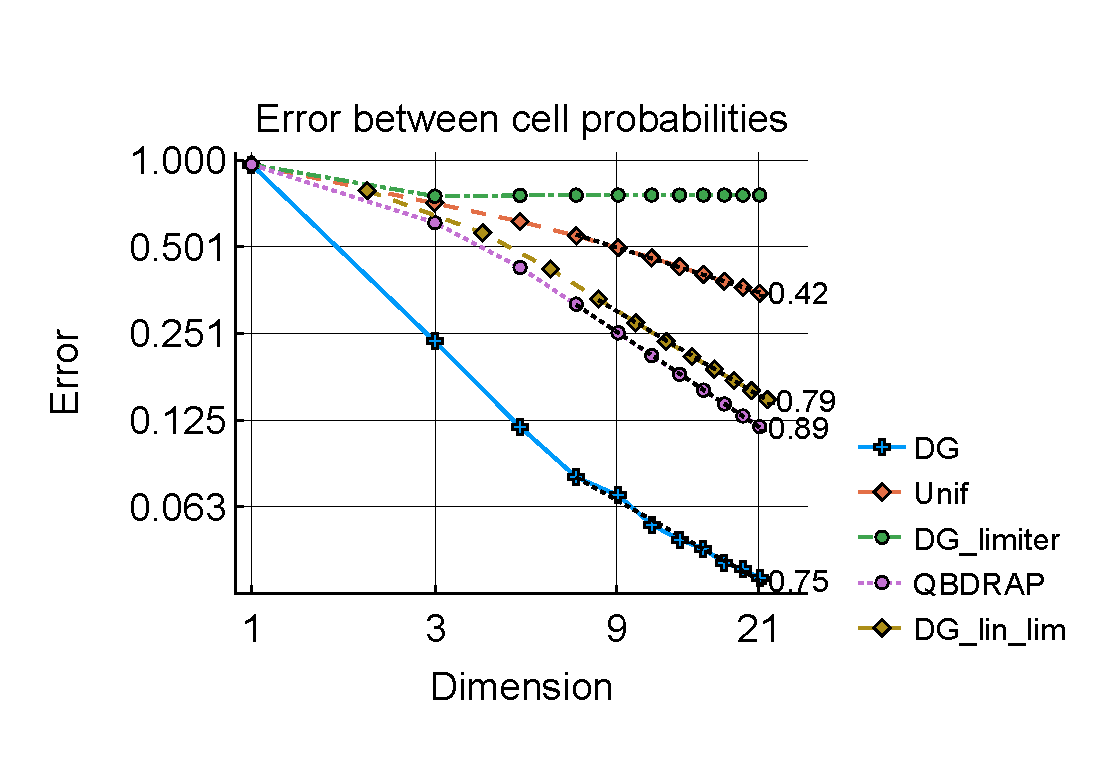
\includegraphics[width=0.5\textwidth,trim={0.75cm 0.8cm 0.25cm 1.25cm},clip]{chapter6/figs/wave/fun1/L1_cell_probs.pdf} 
		\caption{Cell-wise error for the travelling wave problem in Example~\ref{ex: wave 1}. Plotted are the cell-wise errors for the DG (blue solid line), DG-lim (green dashed line), uniformisation (orange dashed line), QBD-RAP (purple dotted line) and DG-lin-lim (gold dashed line) schemes, versus the dimension of the approximation. The black dotted lines are linear least-squares fits to the last 8 data points and the slopes of the least square lines are written next to the last point.}  
		\label{fig: fun 1 wave cp}  
	\end{figure}
	\begin{figure}[h]
		\centering
		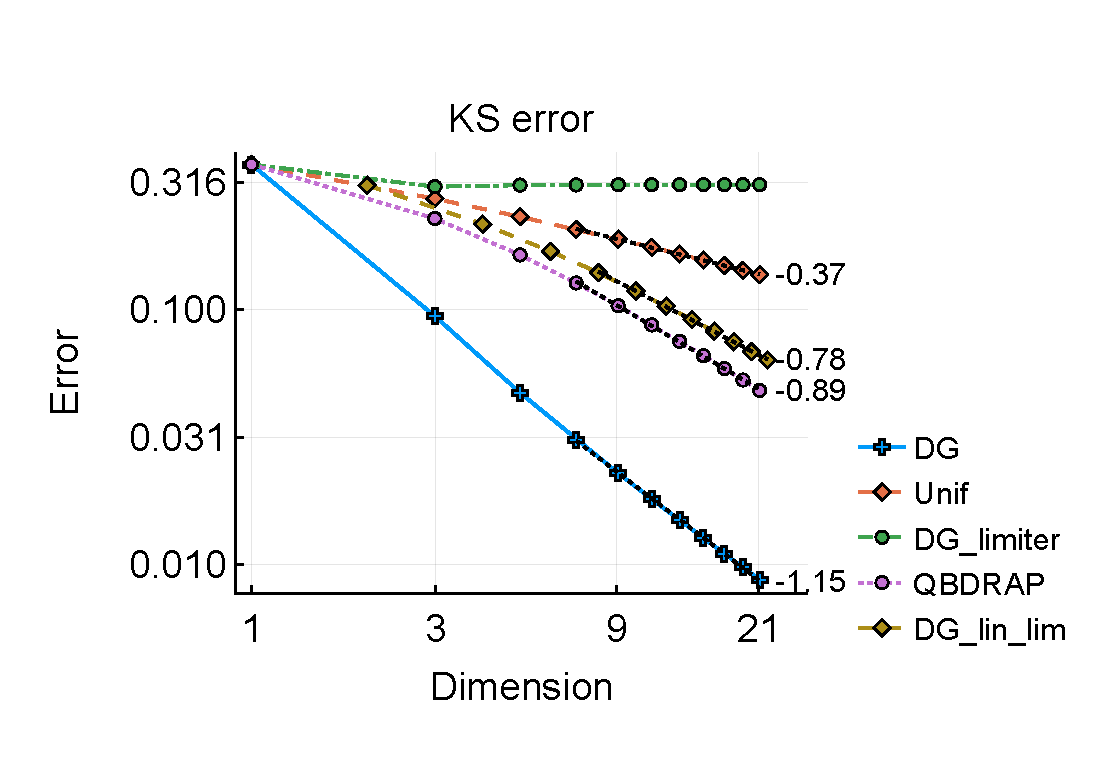
\includegraphics[width=0.5\textwidth,trim={0.75cm 0.8cm 0.25cm 1.25cm},clip]{chapter6/figs/wave/fun1/meshs_ks_error_formatted.pdf}%
		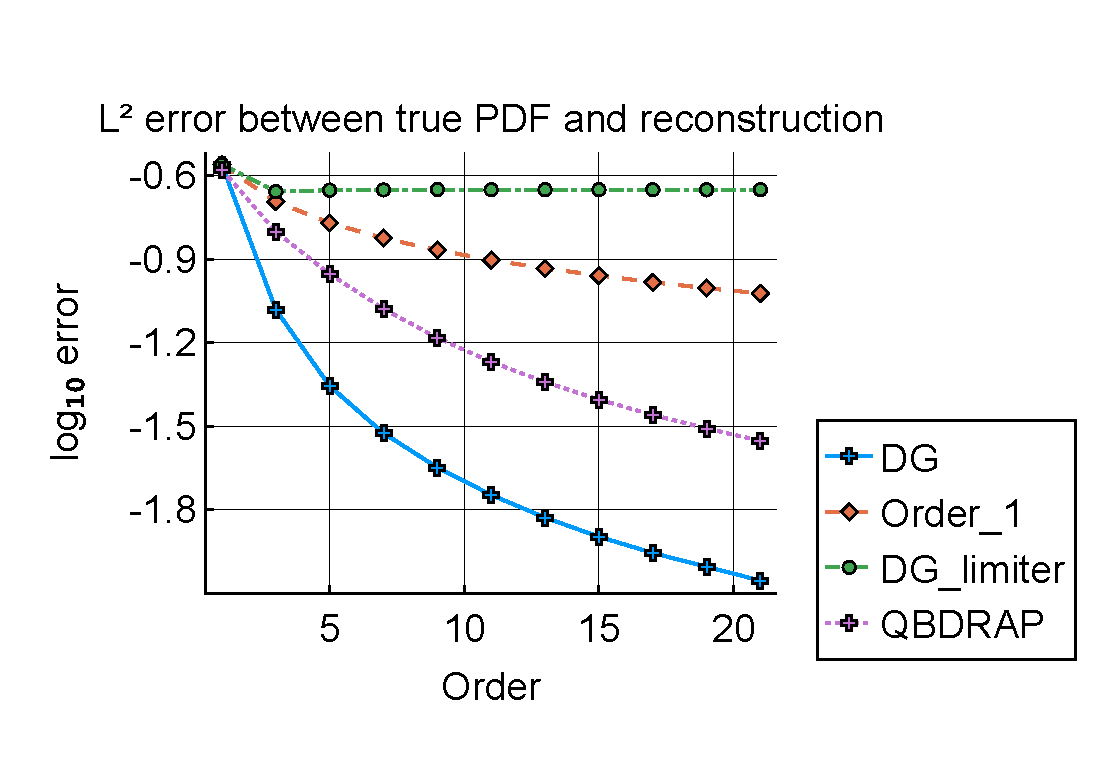
\includegraphics[width=0.5\textwidth,trim={0.75cm 0.8cm 0.25cm 1.25cm},clip]{chapter6/figs/wave/fun1/meshs_l2_pdf_error_formatted.pdf}
		\caption{KS error (left) and \(L^2\) error of the PDF (right) for the travelling wave problem in Example~\ref{ex: wave 1} where approximations are constructed via the DG (blue solid line), DG-lim (green dash-dotted line), uniformisation (orange dashed line), QBD-RAP (purple dotted line) and DG-lin-lim (gold dashed line) schemes. The black dotted lines are linear least-squares fits to the last 8 data points and the slopes of the least square lines are written next to the last point.} 
		\label{fig: fun 1 wave} 
	\end{figure}
	\begin{figure}[h]
		\centering
		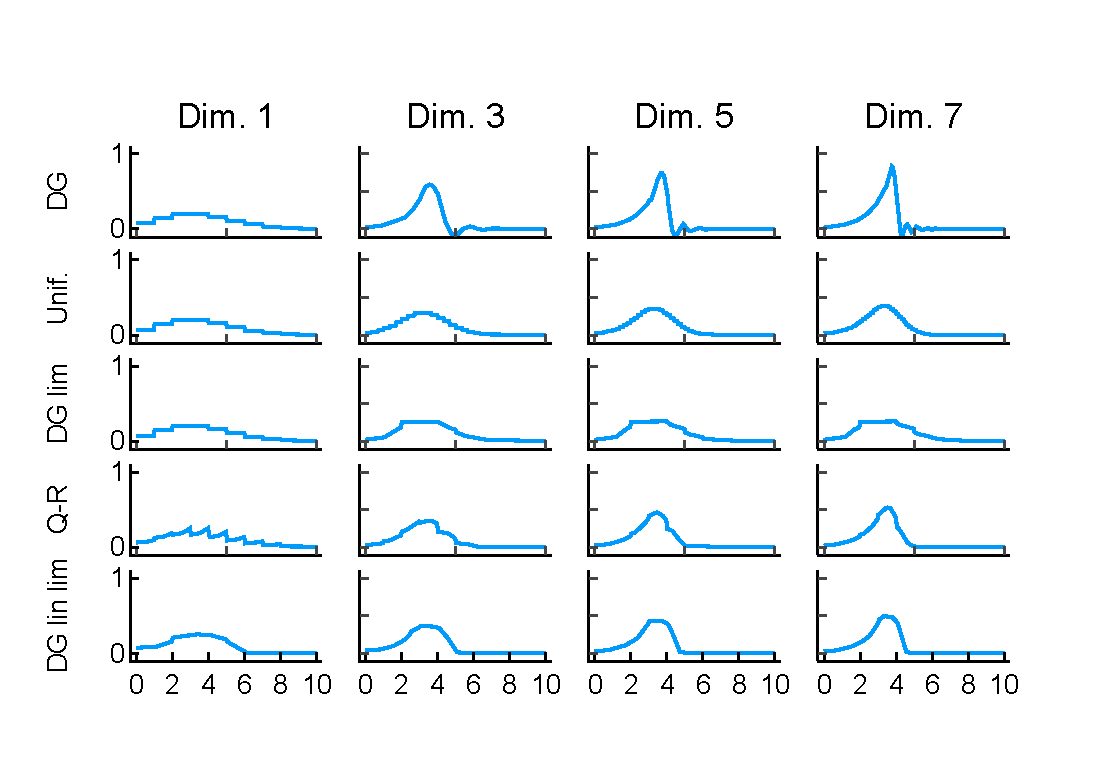
\includegraphics[width=\textwidth,trim={0cm 1.25cm 0cm 1.25cm},clip]{chapter6/figs/wave/fun1/pdf_formatted.pdf}
		\caption{Approximate transient PDFs at time \(t=4\) for Example~\ref{ex: wave 1} using the DG (top row), uniformisation (second row), DG-lim (third row), QBD-RAP (fourth row), and DG-lin-lim (fifth row) schemes of dimensions 1, 3, 5, and 7 (columns). The true density function is \(e^{-(x-4)}1(x<4)\).} 
		\label{fig: pdf wave fun 1}
	\end{figure} 
	%\exampleFloatBarrier
	Figure~\ref{fig: fun 1 wave cp} plots the cell-wise error metric and Figure~\ref{fig: fun 1 wave} plots the KS error (left) and the \(L^2\) error between the PDFs (right). Observing Figures~\ref{fig: fun 1 wave cp} and~\ref{fig: fun 1 wave}, the DG-lim scheme does not perform well, which might be expected due to the discontinuity in the transient distribution at \(x=t<10\) in Phase~1. The uniformisation, DG-lin-lim and QBD-RAP schemes appear to converge, with the QBD-RAP scheme converging fastest, but performing similarly to the DG-lin-lim scheme, and the uniformisation scheme performs the poorest of the three. The DG scheme performs the best, however, produces approximations which are negative and oscillatory as we might expect given the discontinuity. A selection of approximations to the transient PDF are shown in Figure~\ref{fig: pdf wave fun 1}.

	Interestingly, this solution is discontinuous at a cell-edge and even though the DG scheme\footnote{All the schemes considered allow discontinuities at a cell-edges.} allows for discontinuities in the PDF at cell edges, it is unable to capture this discontinuity without producing oscillations. 
\end{example} 

\subsection*{Summary}
We applied the DG, DG-lim, DG-lin-lim, uniformisation and QBD-RAP schemes to travelling wave problems with various initial conditions. All the problems induced oscillations in the DG scheme at some point and as a result the DG-lim scheme reduced the order of the approximation to linear. In some cases, the oscillations in the DG scheme appeared to be transient and were not material in the final approximation. In other cases, the oscillations were present in the final DG approximation causing the approximation to violate the axioms of probability. Of the three positivity preserving alternatives, the DG-lin-lim, uniformisation and QBD-RAP schemes, in general, the uniformisation scheme performs worse than the other two and converges slowly to the true solution. The DG-lin-lim and QBD-RAP schemes perform similarly with the DG-lin-lim scheme performing slightly better for the smoother problems and the QBD-RAP scheme performing slightly better for the problems with more significant discontinuities and point masses. 

This section is the first step in analysing the ability of the approximation schemes to capture the dynamics fluid queues. This section demonstrates that, although the QBD-RAP scheme may have certain deficiencies for solution reconstruction (as demonstrated in Section~\ref{sec: recon num}), it can resolve the movement of probability between cells better than the uniformisation scheme, and similarly compared DG-lin-lim scheme. In the following sections we consider more complicated fluid queue dynamics by introducing some simple stochastic phase changes. 

\FloatBarrier
\section{Limiting distributions} \label{sec:stat}
We briefly turn our attention to limiting distributions of fluid queues. Since the limiting distribution is smooth we expect that the DG scheme will work well here. Moreover, since the solution is smooth, the slope limiter has no effect which means that the DG-lim and DG schemes are equivalent. Analysing the performance of the approximation schemes with the limiting distribution allows us to explore the ability of the schemes to capture the stochastic dynamics, without numerical integration with respect to time. In addition, the limiting distribution is convenient for numerical experiments as we can evaluate it analytically \citep{s2017}, and it does not require us to approximate initial conditions.

Here we analyse a simple model which is based on Example~2 in \cite{bean2009}, except here we add a lower boundary to the model (no lower boundary is specified in Example~2 of \cite{bean2009} as it is inconsequential to their analysis). 

% \begin{model}\label{model: simple}
% 	Consider a fluid queue where the driving process is a CTMC with state space \(\calS=\{1,2,3,4\}\), generator 
% 	\[\bs T = \left[\begin{array}{cccc}
% 		-1.1 & 1.1 & 0 & 0 \\
% 		1 & -1 & 0 & 0 \\ 
% 		0.01 & 0 & -0.01 & 0 \\
% 		0 & 0.01 & 0 & -0.01 
% 	\end{array}\right],\]
% 	and there are associated rates \(c_1=1, c_2 = -1, c_3=0, c_4=0\) and boundaries at \(x=0\) and \(x=10\). We specify two types of behaviour at the boundary.
% 	\begin{enumerate}[a)]
% 		\item (Absorbing model) Upon hitting the lower boundary, the process transitions from phase \(2\) to phase \(j\) with probability \(p_{2j}\) where 
% 		\[\vligne{p_{21} & p_{22} & p_{23} & p_{24}} = \vligne{0 & 0 & 1 & 0}.\]
% 		Upon hitting the upper boundary, the process transitions from phase \(1\) to phase \(j\) with probability \(p_{1j}\) where 
% 		\[\vligne{p_{11} & p_{12} & p_{13} & p_{14}} = \vligne{0 & 0 & 0 & 1}.\]
% 		\item (Reflecting model) Upon hitting the lower boundary, the process transitions from phase \(2\) to phase \(j\) with probability \(p_{2j}\) where 
% 		\[\vligne{p_{21} & p_{22} & p_{23} & p_{24}} = \vligne{1 & 0 & 0 & 0}.\]
% 		Upon hitting the upper boundary, the process transitions from phase \(1\) to phase \(j\) with probability \(p_{1j}\) where 
% 		\[\vligne{p_{11} & p_{12} & p_{13} & p_{14}} = \vligne{0 & 1 & 0 & 0}.\]
% 	\end{enumerate}
% \end{model}
% Phases~3 and 4 are included only to capture behaviour at the boundary.

% For Model~\ref{model: simple}~a), upon hitting the boundary, the process stays at the boundary for an exponentially distributed amount of time with mean 100. For Model~\ref{model: simple}~b), upon hitting the boundary, the process is immediately reflected. In Model~\ref{model: simple}~b) phases 3 and 4 are ephemeral and are included only for notational convenience. 


\begin{model}\label{model: simple}
	Consider a fluid queue where the driving process is a CTMC with state space \(\calS=\{1,2\}\), generator 
	\[\bs T = \left[\begin{array}{cccc}
		-1.1 & 1.1 \\
		1 & -1 \\ 
	\end{array}\right],\]
	and there are associated rates \(c_1=1, c_2 = -1,\) and boundaries at \(x=0\) and \(x=10\). We specify two types of behaviour at the boundary.
	
	Upon hitting the lower boundary, the process immediately transitions from Phase~\(2\) to Phase~\(j\) with probability \(p_{2j}\) where 
		\[\vligne{p_{21} & p_{22} } = \vligne{1 & 0}.\]
	Upon hitting the upper boundary, the process immediately transitions from Phase~\(1\) to Phase~\(j\) with probability \(p_{1j}\) where 
		\[\vligne{p_{11} & p_{12} } = \vligne{0 & 1}.\]
	Thus, upon hitting the boundary, the fluid queue immediately transitions to the other phase and is reflected.
\end{model}

The model was discretised using the DG, uniformisation and QBD-RAP schemes using ten cells of width \(1\). We compute the coefficients for the limiting distribution in the following way. Suppose that a given discretisation scheme results in an approximation to the generator of the fluid queue as a matrix \(\bs B\). Then the limiting coefficients are found by solving 
\begin{align}
	\bs b \bs B = 0,\\
	\mbox{such that } \bs b\bs 1=1,
\end{align}
for the coefficients \(\bs b\). 

% \paragraph{Model~\ref{model: simple}~a) Absorbing model}
% Figure~\ref{fig: absorbing limiting} plots KS errors between the true limiting CDF and the approximations (left) and the \(L^2\) error between the true limiting PDF and the approximations. Clearly the DG scheme is superior here as its error rapidly decreases to a point where is become insignificant compared to other numerical errors. The QBD-RAP scheme and uniformisation scheme both appear to be converging, with the errors for the QBD-RAP scheme decreasing faster.
% \begin{figure}[h]
% 	\centering
% 	\includegraphics[width=0.5\textwidth,trim={0.75cm 0.8cm 0.25cm 1.25cm},clip]{chapter6/figs/hitting_times_model/absorbing_model/limiting_distribution/ks_error_formatted.pdf}%
% 	\includegraphics[width=0.5\textwidth,trim={0.75cm 0.8cm 0.25cm 1.25cm},clip]{chapter6/figs/hitting_times_model/absorbing_model/limiting_distribution/l2_pdf_error_formatted.pdf}
% 	\caption{KS error between the true limiting CDF  and the approximations (left) and \(L^2\) error between the true limiting PDF and the approximations for Model~\ref{model: simple}~a) using the DG scheme (blue solid line), uniformisation scheme (orange dashed line) and QBD-RAP scheme (green dash-dotted line).} 
% 	\label{fig: absorbing limiting} 
% \end{figure}

% \paragraph{Model~\ref{model: simple}.}
\begin{figure}[h]
	\centering
	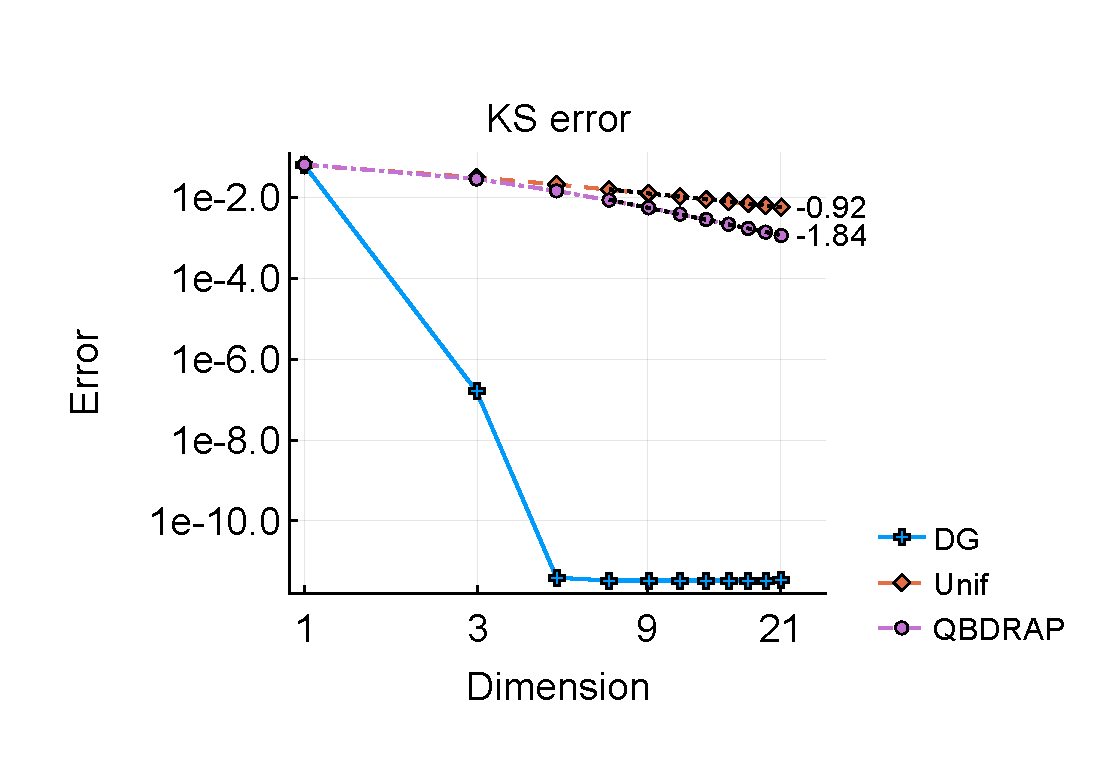
\includegraphics[width=0.5\textwidth,trim={0.75cm 0.8cm 0.25cm 1.25cm},clip]{chapter6/figs/hitting_times_model/reflecting_model/stationary_distribution/ks_error_formatted.pdf}%
	\includegraphics[width=0.5\textwidth,trim={0.75cm 0.8cm 0.25cm 1.25cm},clip]{chapter6/figs/hitting_times_model/reflecting_model/stationary_distribution/l2_pdf_error_formatted.pdf}
	\caption{KS error (left) and \(L^2\) error of the PDF (right) for Model~\ref{model: simple} using the DG (blue solid line), uniformisation (orange dashed line) and QBD-RAP (purple dotted line) schemes. The black dotted lines are linear least-squares fits to the last 8 data points and the slopes of the least square lines are written next to the last point.} 
	\label{fig: reflecting stationary} 
\end{figure}
Figure~\ref{fig: reflecting stationary} plots KS errors between the true limiting CDF and the approximations and the \(L^2\) error between the true limiting PDF and the approximations. Clearly the DG scheme is superior here as its error rapidly decreases to a point where it becomes insignificant compared to other numerical errors. The QBD-RAP and uniformisation schemes both appear to be converging, with the errors for the QBD-RAP scheme decreasing faster.

\FloatBarrier
\section{Transient distributions}\label{sec: transient approx}
Once again we consider Model~\ref{model: simple} and use the same spatial discretisation as described in Section~\ref{sec:stat} (ten cells with width \(\Delta=1\)). Two initial conditions are considered, a point mass with mass 1 at 0 in Phase~1, and the initial distribution with PDF 
\begin{align}
	\cfrac{1}{2}e^{-x}/(1-e^{-10})\label{eqn: exp init cond}
\end{align}
in Phases 1 and 2, with no mass at the boundaries. We numerically integrate over time until time \(t=2.0\) using the SSPRK4 method with t-step size 0.005.\footnote{The \(t\)-step size must be chosen to ensure that numerical integration over time is stable up to dimension 21, adhering to a CFL-like condition \cite[Section~4.8]{nodalDGBook}.} Here we use the DG scheme without a limiter and the DG-lin-lim scheme. Error plots for the DG-lim scheme are included for completeness, but we do not comment on them in detail in this section due to their poor performance for discontinuous problems which we noted previously.

To obtain a \emph{ground truth} \(5\times 10^{10}\) realisations of the fluid queue were simulated until \(t=2\), then the empirical CDF and the masses within each cell were computed from the simulations. We denote the empirical probability distribution by \(\mathbb P_{sim}\). We then compute the KS and \(L^1\) error metrics between the approximated and simulated CDFs, as well as the cell-wise error metric, given as follows. 
\begin{align}
	&\sum_{j\in\{1,2\}}\sum_{\ell=1}^{10} \left|\mathbb P_{sim}(X(2)\in\calD_{\ell,j}, \varphi(2)=j\mid X(0)=0.5,\varphi(0)=1)-p(2,\ell,j)\right|\nonumber 
	\\&+\left|\mathbb P_{sim}(X(2)\in\{10\}, \varphi(2)=4\mid X(0),\varphi(0))-p(2,11,4)\right|\nonumber 
	\\&+\left|\mathbb P_{sim}X(2)\in\{0\}, \varphi(2)=3\mid X(0),\varphi(0))-p(2,0,3)\right| \label{eqn: cell errors 2}
\end{align}
where \(p(2,\ell,j)\) is an approximation to \(\mathbb P_{sim}(X(2)\in\calD_{\ell,j}, \varphi(2)=j\mid X(0),\varphi(0))\), \(p(2,11,4)\) is an approximation to \(\mathbb P_{sim}(X(2)\in\{10\}, \varphi(2)=4\mid X(0),\varphi(0))\), and \(p(2,0,3)\) is an approximation to \(\mathbb P_{sim}(X(2)\in\{0\}, \varphi(2)=3\mid X(0),\varphi(0))\).

To account for possible Monte-Carlo error, we used a bootstrap with 1,000 bootstrap samples. For the bootstrap we sample \(5\times 10^{10}\) realisations of the fluid queue with replacement from the original \(5\times 10^{10}\) samples, then compute error metrics with the resampled data. We resample 1,000 times, resulting in 1,000 estimates of the errors. Via the bootstrap, we report the \(5\)th and \(95\)th percentile of the sampling distribution of the errors. 

To evaluate error metrics, we use a grid of 10,001 evenly spaced points for each phase.

To approximate the point mass initial condition we compute the initial coefficients for each scheme exactly. For the exponential initial condition in (\ref{eqn: exp init cond}) we compute the initial coefficients via Gauss-Lobatto quadrature for the DG scheme, by using the mid-point rule for the uniformisation scheme, and by using a trapezoidal rule with 2,001 points on each cell for the QBD-RAP scheme. 

\paragraph{Model~\ref{model: simple} with exponential initial condition}
\begin{figure}[h]
	\centering
	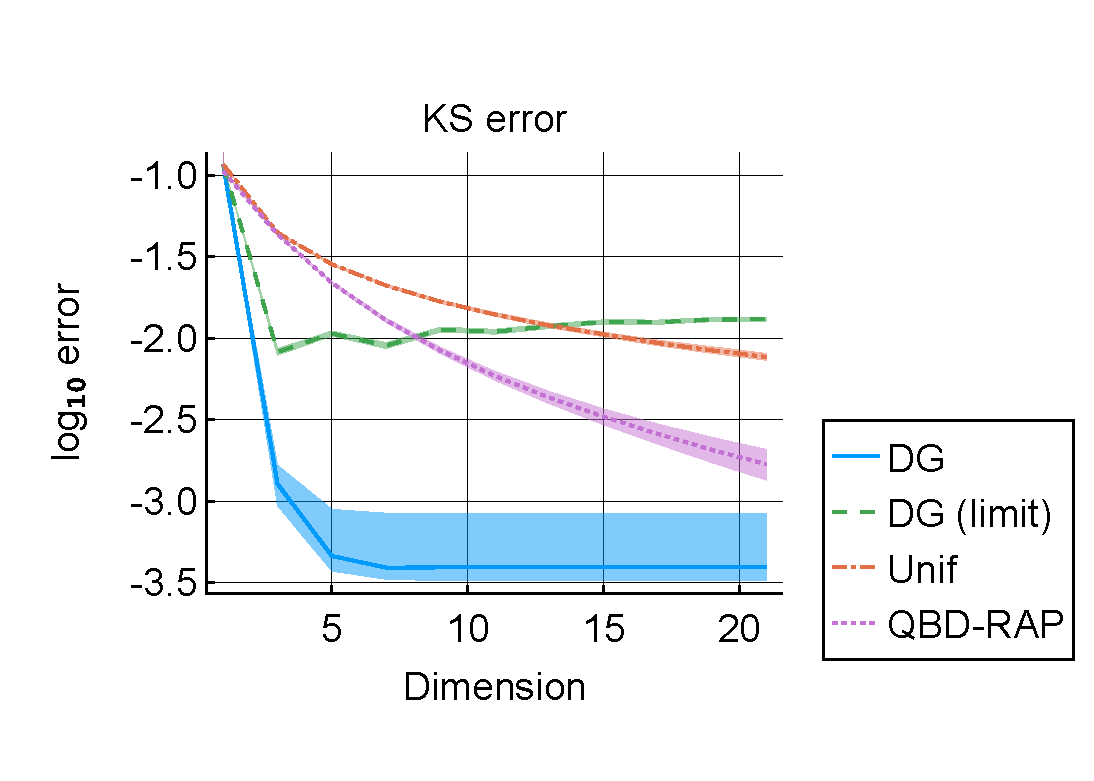
\includegraphics[width=0.5\textwidth,trim={0.75cm 0.8cm 0.25cm 1.25cm},clip]{chapter6/figs/hitting_times_model/reflecting_model/transient_distribution/exp/ks_error_formatted.pdf}%
	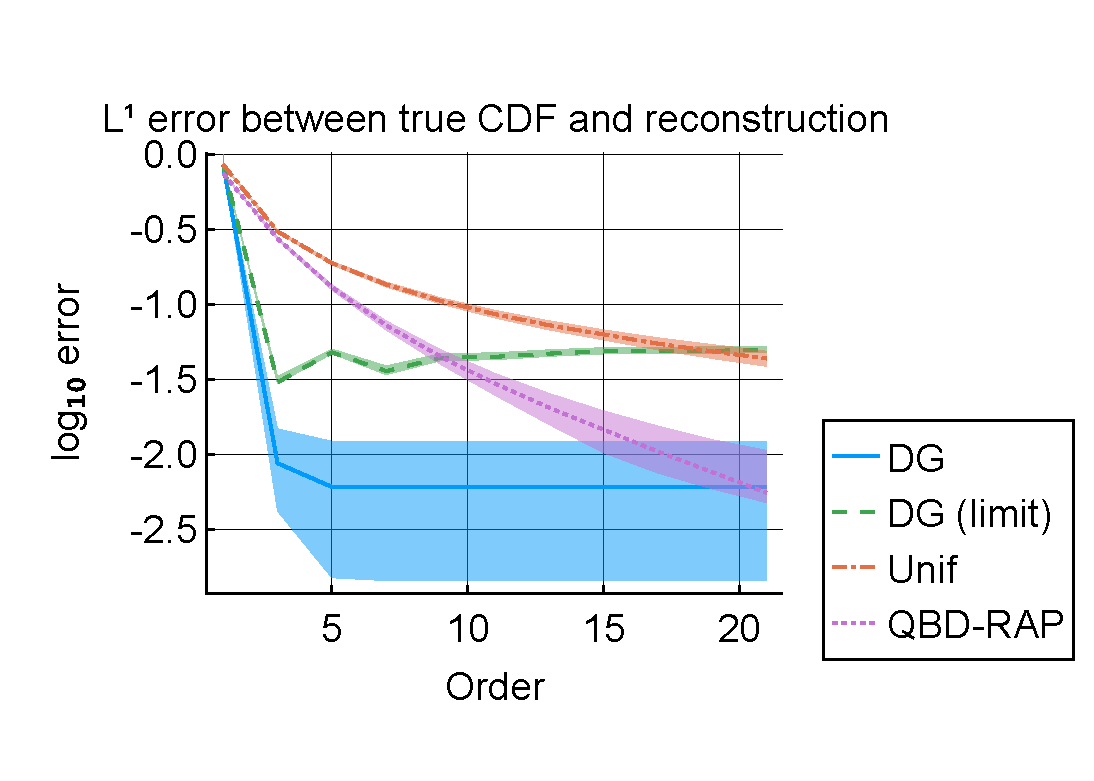
\includegraphics[width=0.5\textwidth,trim={0.75cm 0.8cm 0.25cm 1.25cm},clip]{chapter6/figs/hitting_times_model/reflecting_model/transient_distribution/exp/l1_cdf_error_formatted.pdf}
	\caption{KS (left) and \(L^1\) (right) errors between the true transient CDF at time \(t=2\) for Model~\ref{model: simple} with the exponential initial condition, where the approximations were obtained via the DG (blue solid line), DG-lim (green dashed line), uniformisation (orange dashed line), QBD-RAP (purple dotted line) and DG-lin-lim (gold dashed line) schemes. Bootstrapped 90\% confidence intervals are shown by the lighter coloured strip surrounding the lines. The black dotted lines are linear least-squares fits to the last 8 data points and the slopes of the least square lines are written next to the last point.} 
	\label{fig: reflecting transient exp} 
\end{figure}
Figure~\ref{fig: reflecting transient exp} shows the KS and \(L^1\) metric on the CDF for the five different schemes (DG, DG-lim, DG-lin-lim, uniformisation and QBD-RAP schemes). For both error metrics the DG scheme converges rapidly until computational/simulation errors become significant. The uniformisation, DG-lin-lim and QBD-RAP schemes converge at a slower rate than the DG scheme, with the QBD-RAP and DG-lin-lim schemes converging faster than the uniformisation scheme. For the KS metric, the DG-lin-lim scheme outperforms the QBD-RAP scheme at all dimensions, while for the \(L^1\) metric, the two schemes perform similarly. 

The DG-lim does not appear to be converging, which suggests there is at least one iteration during the numerical integration over time at which the numerical solution displays oscillations. However, when the DG approximations for the distribution at time \(t=2\) are plotted, they do not appear to display oscillations (not shown). This suggests that the oscillations which might occur with the DG scheme are transient, and have dissipated by time \(t=2\). The oscillations which the limiter detects in the DG scheme are likely from the reflecting boundary at \(x=0\). In the early stages of the evolution of the model the majority of the density in Phase~2 near zero will move to the left at rate 1 and hit the boundary at \(x=0\). Upon hitting the boundary, the density is reflected into Phase~1. Meanwhile, the initial density in Phase~1 moves to the right at rate 1 and the density reflected at the boundary from Phase~2 fills in to the region between \(x=0\) and \(x=t\) in Phase~1. Intuitively, in the early evolution of the model, there will be a sharp peak in the transient density at \(x=t\). The true transient density is continuous, but not differentiable, at the point \(x=t\) for \(t<10\).  %

\begin{figure}[h]
	\centering
	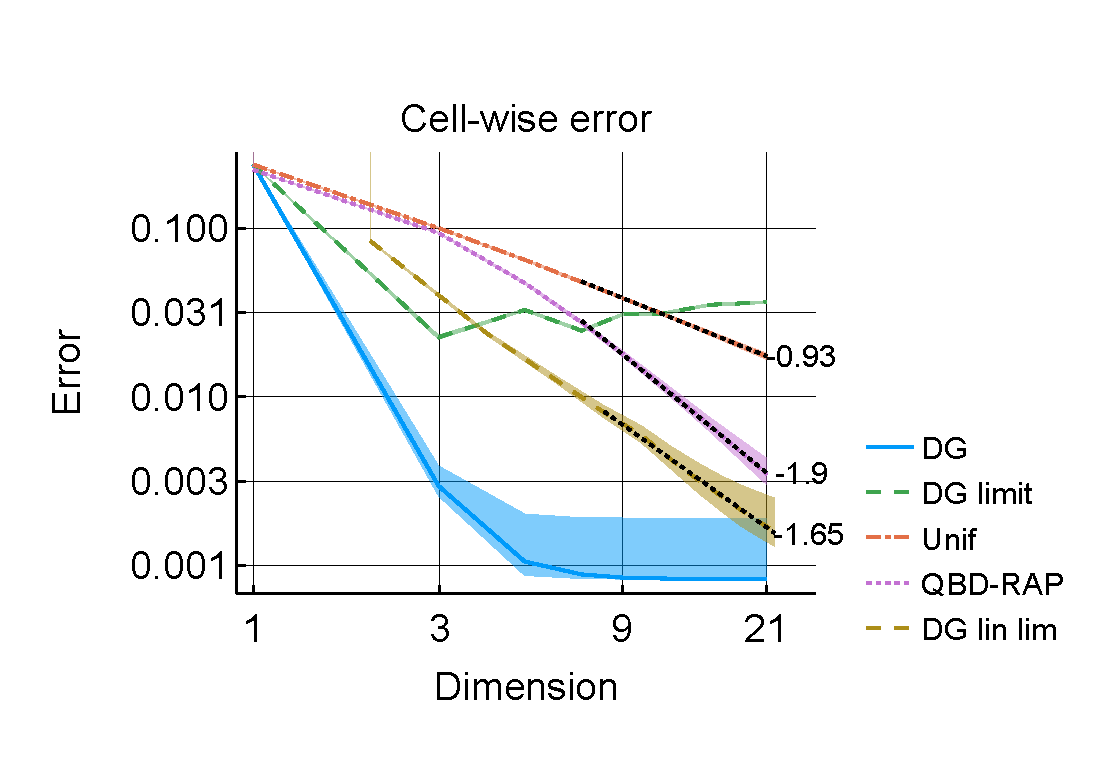
\includegraphics[width=0.5\textwidth,trim={0.75cm 0.8cm 0.25cm 1.25cm},clip]{chapter6/figs/hitting_times_model/reflecting_model/transient_distribution/exp/L1_cell_probs_error_formatted.pdf}
	\caption{Cell-wise error metric from (\ref{eqn: cell errors 2}) for Model~\ref{model: simple} with the exponential initial condition, where the approximations were obtained via the DG (blue solid line), DG-lim (green dashed line), uniformisation (orange dashed line), QBD-RAP (purple dotted line) and DG-lin-lim (gold dashed line) schemes. Bootstrapped 90\% confidence intervals are shown by the lighter coloured bars surrounding the lines. The black dotted lines are linear least-squares fits to the last 8 data points and the slopes of the least square lines are written next to the last point.} 
	\label{fig: reflecting transient exp cp} 
\end{figure}
%\exampleFloatBarrier
Figure~\ref{fig: reflecting transient exp cp} plots the cell-wise error metric (\ref{eqn: cell errors 2}) for Model~\ref{model: simple} with the exponential initial condition. Since the cell-wise errors do not require us to reconstruct the value of the solution within each cell, this metric allows us to observe the error characteristics of the schemes without reconstruction. Figure~\ref{fig: reflecting transient exp cp} shows similar convergence characteristics to the KS error metric in Figure~\ref{fig: reflecting transient exp} (left). 

\paragraph{Model~\ref{model: simple} with a point-mass initial condition}
\begin{figure}[h]
	\centering
	% 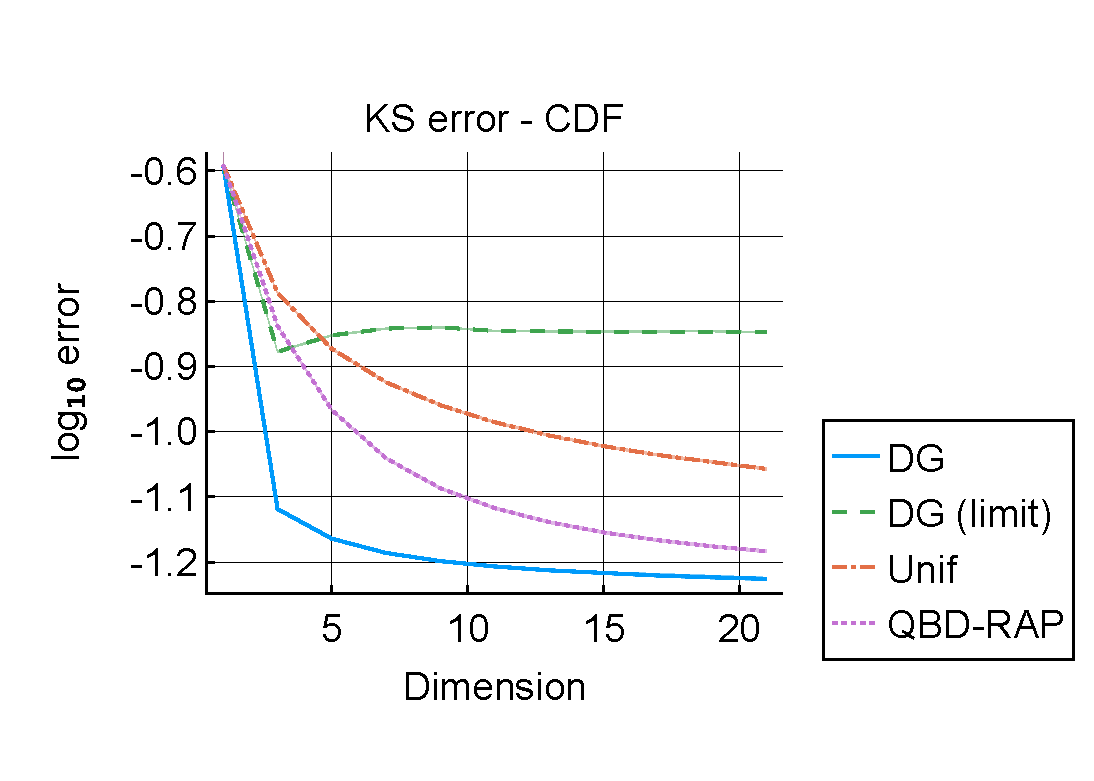
\includegraphics[width=0.5\textwidth,trim={0.75cm 0.8cm 0.25cm 1.25cm},clip]{chapter6/figs/hitting_times_model/reflecting_model/transient_distribution/point_mass/ks_error_formatted.pdf}%
	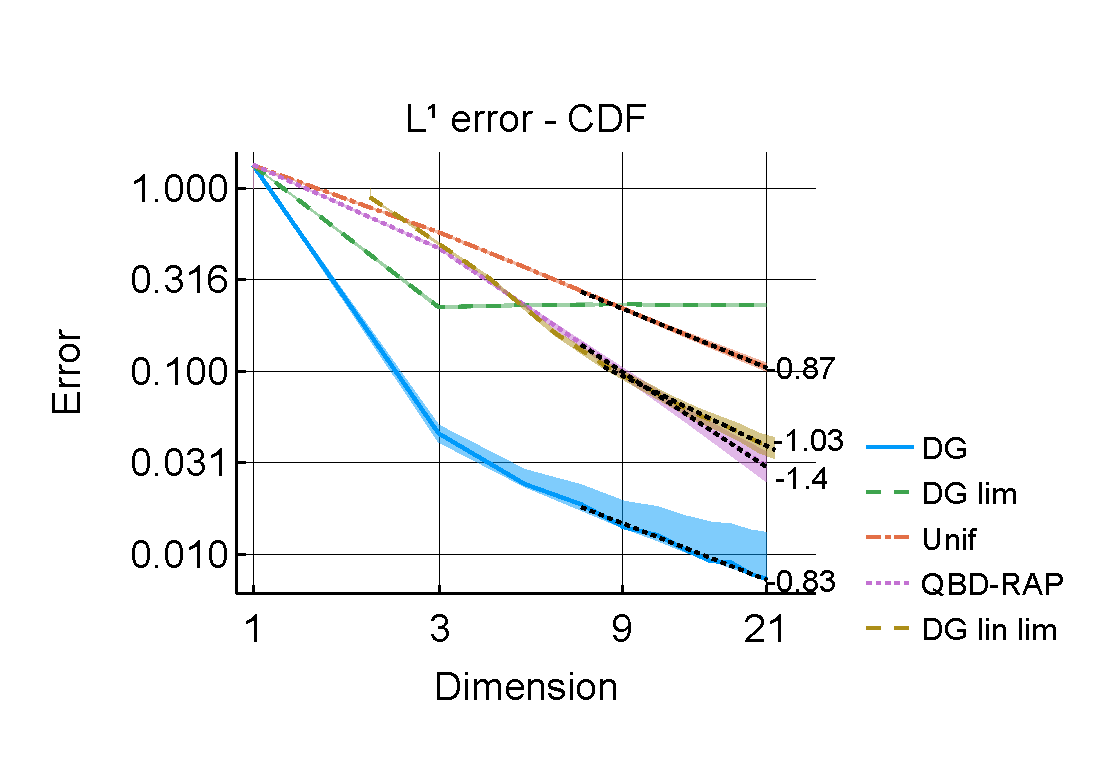
\includegraphics[width=0.5\textwidth,trim={0.75cm 0.8cm 0.25cm 1.25cm},clip]{chapter6/figs/hitting_times_model/reflecting_model/transient_distribution/point_mass/l1_cdf_error_formatted.pdf}%
	\includegraphics[width=0.5\textwidth,trim={0.75cm 0.8cm 0.25cm 1.25cm},clip]{chapter6/figs/hitting_times_model/reflecting_model/transient_distribution/point_mass/L1_cell_probs_error_formatted.pdf}
	% \caption{KS (left) and \(L^1\) (right) errors between the CDF at time \(t=2\) for Model~\ref{model: simple} with the point-mass initial condition, where the approximations were obtained via the DG (blue solid line), DG-lim (green dashed line), uniformisation (orange dashed line), QBD-RAP (purple dotted line) and DG-lin-lim (gold dashed line) schemes. Bootstrapped 90\% confidence intervals are shown by the lighter coloured bars surrounding the lines. The black dotted lines are linear least-squares fits to the last 8 data points and the slopes of the least square lines are written next to the last point.} 
	\caption{\(L^1\) errors between the CDF, and cell-wise errors, at time \(t=2\) for Model~\ref{model: simple} with the point-mass initial condition, where the approximations were obtained via the DG (blue solid line), DG-lim (green dashed line), uniformisation (orange dashed line), QBD-RAP (purple dotted line) and DG-lin-lim (gold dashed line) schemes. Bootstrapped 90\% confidence intervals are shown by the lighter coloured bars surrounding the lines. The black dotted lines are linear least-squares fits to the last 8 data points and the slopes of the least square lines are written next to the last point.} 
	\label{fig: reflecting transient pm} 
\end{figure}
Figure~\ref{fig: reflecting transient pm} (left) shows \(L^1\) error on the CDF for the five different schemes (DG, DG-lim, DG-lin-lim, uniformisation and QBD-RAP schemes). Comparing the \(L^1\) error metrics in Figure~\ref{fig: reflecting transient pm} for the point mass initial condition with the ones in Figure~\ref{fig: reflecting transient exp} for the exponential initial condition all schemes perform worse for the point mass initial condition. Regarding comparative convergence of error for this problem, for both error metrics the DG scheme converges fastest, followed by the QBD-RAP and DG-lin-lim schemes which converge comparatively, then the uniformisation scheme. For the DG scheme, the rate at which the error decreases as the dimension of the scheme increases slows significantly after dimension 3. This is likely due to the DG scheme approximating smooth regions of the solution well when the dimension is 3 or greater, after which the majority of the error is due to the discontinuity in the solution, for which the rate of convergence is slower. 
%

% \begin{figure}[h]
% 	\centering
% 	\includegraphics[width=0.5\textwidth,trim={0.75cm 0.8cm 0.25cm 1.25cm},clip]{chapter6/figs/hitting_times_model/reflecting_model/transient_distribution/point_mass/L1_cell_probs_error_formatted.pdf}
% 	\caption{Cell-wise errors for Model~\ref{model: simple} at time \(t=2\) with the point mass initial condition, where the approximations were obtained via the DG (blue solid line), DG-lim (green dashed line), uniformisation (orange dashed line), QBD-RAP (purple dotted line) and DG-lin-lim (gold dashed line) schemes. Bootstrapped 90\% confidence intervals are shown by the lighter coloured bars surrounding the lines.} 
% 	\label{fig: reflecting transient pm cp} 
% \end{figure}%
\begin{figure}[h]
	\centering
	\includegraphics[width=0.5\textwidth,trim={0.75cm 0.8cm 0.25cm 1.25cm},clip]{chapter6/figs/hitting_times_model/reflecting_model/transient_distribution/point_mas_t_2.1/L1_cell_probs_error_formatted.pdf}
	\caption{Cell-wise errors for Model~\ref{model: simple} at time \(t=2.1\) with the point mass initial condition, where the approximations were obtained via the DG (blue solid line), DG-lim (green dashed line), uniformisation (orange dashed line), QBD-RAP (purple dotted line) and DG-lin-lim (gold dashed line) schemes. Bootstrapped 90\% confidence intervals are shown by the lighter coloured bars surrounding the lines. The black dotted lines are linear least-squares fits to the last 8 data points and the slopes of the least square lines are written next to the last point.} 
	\label{fig: reflecting transient pm t2.1} 
\end{figure}
\begin{figure}[h]
	\centering
	\includegraphics[width=0.8\textwidth,trim={0cm 1.25cm 0cm 1.25cm},clip]{chapter6/figs/hitting_times_model/reflecting_model/transient_distribution/point_mas_t_2.1/order_21_CDFs_formatted.pdf}
	\caption{Dimension 21 QBD-RAP and dimension 22 DG-lin-lim approximations to the CDF in Phase~1 for Model~\ref{model: simple} with a point-mass initial condition. An empirical estimate of the CDF obtained via simulation is plotted in grey.}  
	\label{fig: reflecting transient pm t2.1 cdfs} 
\end{figure}
Figure~\ref{fig: reflecting transient pm} (right) plots the cell-wise error metric (\ref{eqn: cell errors 2}) for Model~\ref{model: simple} with the point mass initial condition. Figure~\ref{fig: reflecting transient pm} (right) suggests that approximating the cell-wise probabilities seems to be a difficult problem. This is likely caused by the discontinuity at \(x=2\) in Phase \(1\), which lies exactly on a cell boundary. To investigate how the position of the discontinuity might affect the error metrics we evolved the model to time \(t=2.1\) and computed the \(L^1\) error between the CDFs and the cell-wise error. Once again, we use simulation and bootstrapping to approximate the true distribution. The plot (not shown) of the \(L^1\) error between the CDFs for the model at times \(t=2\) and \(t=2.1\) is relatively similar to the one shown and not noteworthy. The plot of the cell-wise error metric at time \(t=2.1\) in Figure~\ref{fig: reflecting transient pm t2.1} is somewhat more interesting. Firstly, Figure~\ref{fig: reflecting transient pm t2.1} shows that all schemes improved from time \(t=2\) to time \(t=2.1\) with respect to this metric. Figure~\ref{fig: reflecting transient pm t2.1} also shows that the cell-wise error metric is somewhat volatile for the DG scheme; this is due to the oscillations in the DG approximation. In contrast, in Figure~\ref{fig: reflecting transient pm t2.1} the uniformisation and QBD-RAP schemes have monotonically decreasing error curves. Also interesting is the DG-lin-lim scheme, which does not improve past dimension 7. It seems that the discontinuity at \(x=t\) is not easily resolved by the scheme given the presence of the limiter. Figure~\ref{fig: reflecting transient pm t2.1 cdfs} plots the CDFs in Phase~1 around the discontinuity in the transient distribution at time \(t=2.1\) for the dimension 21 QBD-RAP and dimension 22 DG-lin-lim schemes. Neither scheme does a particularly good job of capturing the discontinuity, but the QBD-RAP scheme appears to perform slightly better. 


\subsection*{Summary}
For the exponential initial condition the DG scheme performed well, producing the lowest errors. This was followed by the DG-lin-lim scheme, then the QBD-RAP scheme, then the uniformisation scheme, while the DG-lim scheme did not perform well at all. The fact that the DG-lim scheme did not perform well suggests that there must have been oscillations in the DG solution at some point, although these oscillations are not obvious in the DG approximation at time \(t=2\). In general the methods all performed better for the exponential initial condition than for the point mass initial condition. For the point mass initial condition the DG scheme produced oscillatory solutions. Of the viable positivity preserving methods the uniformisation scheme appears to be converging but at a slower rate than the DG-lin-lim and QBD-RAP schemes. Of the two best performing positivity preserving schemes, the QBD-RAP scheme performed slightly better for the point mass initial condition, while the DG-lin-lim scheme performed slightly better for the exponential initial condition. 

This section investigated the performance of the approximation schemes for a simple fluid queue. In the next section we analyse the approximation schemes in more detail by investigating their ability to approximate hitting times of fluid queues. 

\FloatBarrier
\section{Hitting times}\label{sec: hit approx}
We can gain further insight into the approximation schemes by investigating how they perform approximating hitting times of fluid queues. This is also an important aspect to consider if we wish to apply the schemes to approximate operators from the analysis fluid-fluid queues. Recall, in the analysis of fluid-fluid queues in Section~\ref{sec: ffq intro}, we partition sample paths of the second fluid into periods where it is either increasing, decreasing, or constant. The position of \((X(t),\varphi(t))\) determines the rate at which the second fluid moves, hence the hitting times on the boundaries of the sets \(\mathcal F_i^+, \mathcal F_i^-,\) and \(\mathcal F_i^0\) determine the periods of time when the second fluid is either increasing, decreasing, or constant.

Once again we consider Model~\ref{model: simple}. Let \(\zeta_{X}(\{0,1\}) = \{\inf t>0 \mid X(t)=0, \mbox{ or }X(t)=1\},\) be the first hitting time of \(\{X(t)\}\) on the set \(\{0,1\}\). The distribution of the hitting time in phase \(i\in\{1,2\}\) is 
\begin{equation}\label{eqn: hit cdf}\mathbb P(\zeta_{X}(\{0,1\}) < t, \varphi(t)=i\mid \bs X(0)\sim \mu),\end{equation}
for some initial distribution \(\mu\). We look at two initial conditions; an exponential with equal mass in each phase, 
\[\mathbb P(X(0)\in\wrt x,\varphi(0)=i) = \cfrac{1}{2}\cfrac{e^{-x}}{(1-e^{-1})},\,i\in\{1,2\},\]
and a point mass at \(X(0)=0\) in phase \(\varphi(0)=1\). 

We partition the interval \([0,1]\) into three intervals of width \(1/3\). To capture the mass which has hit the set \(\{0,1\}\), we suppose that when the process hits \(\{0\}\) or \(\{1\}\) it is absorbed forever and remains in the phase in which the process first hit \(\{0\}\) or \(\{1\}\). We integrate the schemes until time \(t=10\) using the SSPRK4 method with \(t\)-step size 0.005/3.\footnote{Since we use a smaller cell-width in this example than in previous examples we need to reduce the \(t\)-step size accordingly to ensure that numerical integration is stable for schemes up to dimension 21, adhering to a CFL-like condition \cite[Section~4.8]{nodalDGBook}.} We use the DG scheme with and without a slope limiter during the time-integration and implement both the DG-lim and DG-lin-lim schemes. At each time-step of the numerical integration, we record the amount of mass at the absorbing boundaries in each phase, which gives us an approximation of the cumulative distribution function of the hitting time in each phase, up to time \(t=10\). 

As a \emph{ground truth} we simulate \(5\times 10^{10}\) realisations and record the hitting time on the set \(\{0,1\}\) and the phase at the time of hitting. We then compute the empirical CDF of the hitting probabilities 
\[\mathbb P(\zeta_{X}(\{0,1\}) < t, \varphi(t)=i\mid \bs X(0)\sim \mu),\] 
for \(t=0.005/3\times k\), \(k=0,...,6000\). 

To account for Monte-Carlo errors we take 1,000 bootstrap resamples of the original \(5\times 10^{10}\) samples and compute the empirical CDF of the hitting times for each bootstrap sample. For each bootstrap sample, we resample \(5\times 10^{10}\) points with replacement from the original \(5\times 10^{10}\) realisations, then compute the error metrics between the empirical and approximate CDFs and, ultimately, estimate the 5th and 95th percentile of the distribution of the errors. 

\paragraph{Exponential initial condition}
\begin{figure}[h]
	\centering
	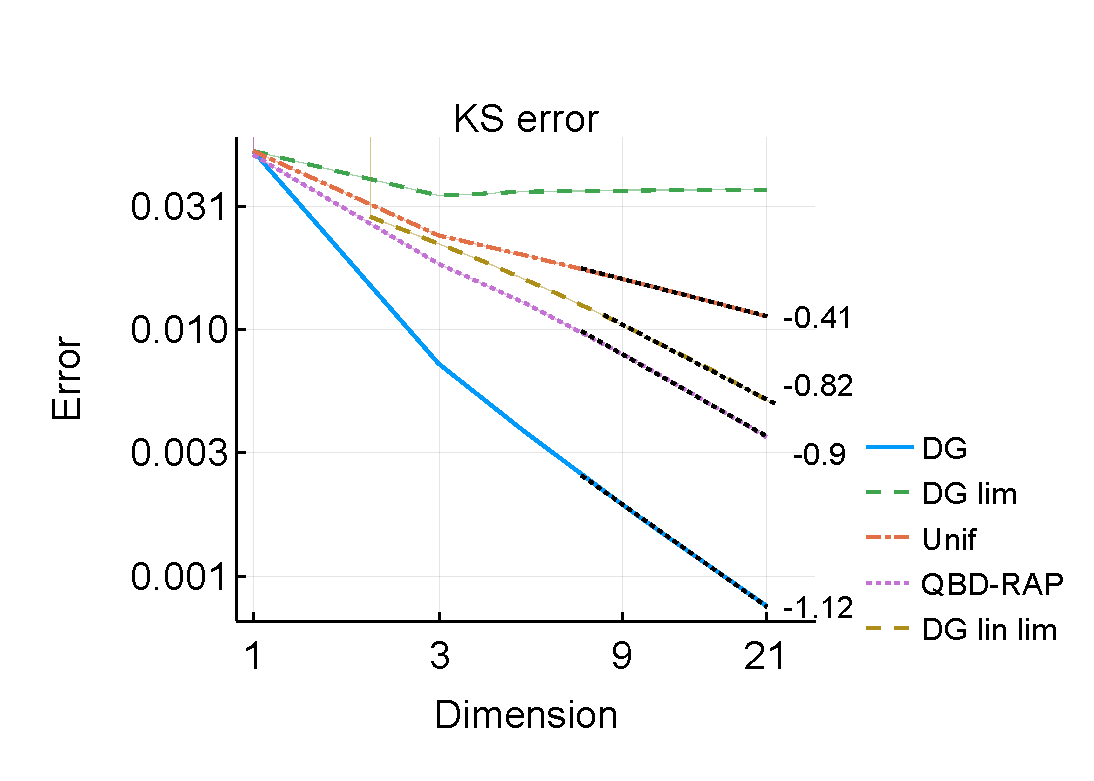
\includegraphics[width=0.5\textwidth,trim={0.75cm 0.8cm 0.25cm 1.25cm},clip]{chapter6/figs/hitting_times_model/hitting_times/exp/ks_error_formatted.pdf}%
	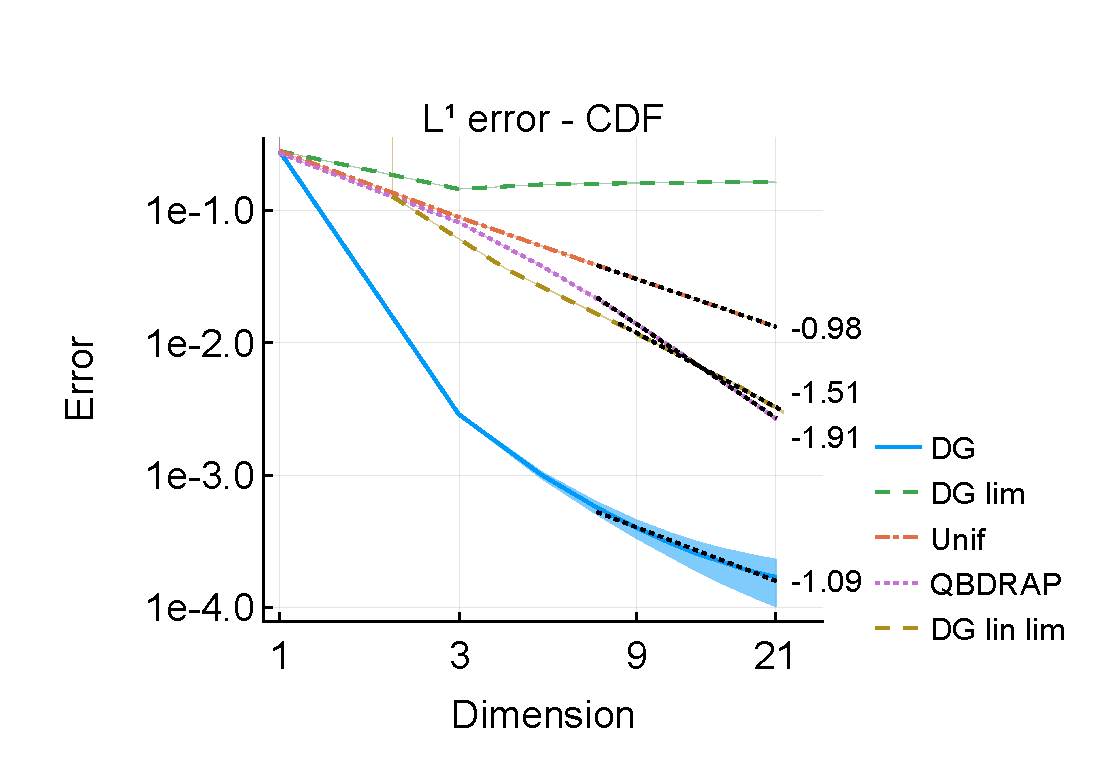
\includegraphics[width=0.5\textwidth,trim={0.75cm 0.8cm 0.25cm 1.25cm},clip]{chapter6/figs/hitting_times_model/hitting_times/exp/l1_cdf_error_formatted.pdf}
	\caption{KS (left) and \(L^1\) (right) errors between the simulated and approximate first hitting time CDFs in (\ref{eqn: hit cdf}) for Model~\ref{model: simple} with the exponential initial condition. The approximations were obtained via the DG (blue solid line), DG-lim (orange dashed line), uniformisation (green dashed line), QBD-RAP (purple dotted line) and DG-lin-lim (gold dashed line) schemes. Bootstrapped 90\% confidence intervals are shown by the lighter coloured bars surrounding the lines. The black dotted lines are linear least-squares fits to the last 8 data points and the slopes of the least square lines are written next to the last point.}
	\label{fig: hitting time exp} 
\end{figure}
Figure~\ref{fig: hitting time exp} shows the error metrics recorded for the five numerical approximation schemes applied to the hitting time problem with the exponential initial condition. For both error metrics the DG scheme performs the best. 

The DG-lim scheme does not appear to converge, suggesting oscillations in the DG approximation. With this initial condition the transient distribution of the fluid queue on the event that it remains in the interval \((0,1)\) is discontinuous at \(x=t\) in Phase~1 and \(x=1-t\) in Phase~2 for \(x,t<1\). There is also a discontinuity in the hitting time PDF at time \(t=1\). 

Regarding the other positivity preserving schemes, the uniformisation, DG-lin-lim and QBD-RAP schemes, all appear to converge, with the QBD-RAP and DG-lin-lim schemes performing similarly and better than the uniformisation scheme. 

In Figure~\ref{fig: hitting time oscillation exp} we plot the PDFs of the hitting times \(\zeta_X(\{0,1\})\), in each phase, for the dimension 21 DG, dimension 21, QBD-RAP and dimension 22 DG-lin-lim schemes. Figure~\ref{fig: hitting time oscillation exp} demonstrates oscillations in the DG approximation, though the PDF is not negative in this case. All schemes seem to capture the discontinuity at \(t=1\) relatively well. There is an interesting artefact in the QBD-RAP approximation around \(t=0\) where the scheme has generated an oscillation. Let us investigate this artefact further. 

Intuitively, most sample paths which exit near \(t=0\) start near a boundary, they see a change of phase shortly after \(t=0\), then remain in that phase until hitting \(\{0,1\}\). Consider such a sample path which starts at \(x_0=0\) in Phase~1 and exits at time \(v\) with a single change of phase at time \(u\in(0,v)\). For the fluid queue, \(u=v/2\), and we want the QBD-RAP scheme to approximate this. The QBD-RAP approximation to this sample paths has density\footnote{One significant advantage of the QBD-RAP and uniformisation approaches is that, from their stochastic interpretation, we can use sample-path arguments to analyse the scheme.} 
\begin{align}
	\bs \alpha e^{(\bs S - \bs I)u} \bs D e^{(\bs S - 1.1\bs I)(v-u)}\bs s = \bs \alpha e^{\bs Su} \bs D e^{\bs S(v-u)}\bs s e^{-1.1v+0.1u}.\label{eqn :lf}
\end{align}
We want (\ref{eqn :lf}) to approximate a point mass at \(v=2u\). To see that this is the case, recall that we can approximate a point mass at \(u\) by 
\begin{equation}\bs k(\Delta - u)\bs e^{\bs Sx}\bs s,\label{eqn:aafba}\end{equation}
where \(\bs k(z)=\cfrac{\bs \alpha e^{\bs Sz}}{\bs \alpha e^{\bs Sz\bs e}}\),
and recall that the matrix \(\bs D\) is an approximation; 
\begin{align}
	\bs \alpha e^{\bs Su}\bs D &= \mathbb E\left[\bs k(Z-u)1(Z>u)\right]\nonumber 
	% \\&\approx \bs \alpha e^{\bs S(v-u)}\bs e \bs k(\Delta-(v-u))
	\\&\approx\mathbb P(Z>u) \bs k(\Delta-u), \label{eqn: aegpb}
\end{align} where \(Z\sim ME(\bs \alpha,\bs S)\)
and \(Z\) is concentrated around \(\Delta\). 

Thus, (\ref{eqn :lf}) is approximately  
\[e^{-1.1v+0.1u} \mathbb P(Z>u) \bs k(\Delta-u)\bs e^{\bs S(v-u)}\bs s,\]
which approximates a point mass at \(v-u=u\), or \(2u=v\). Retracing our arguments, sources of error in this approximation come from the approximation in (\ref{eqn: aegpb}) and from the approximation of a point mass by (\ref{eqn:aafba}), which we commented on in Section~\ref{sec: closing vecs numerics} where we conducted numerical experiments about the unnormalised closing operator given by \(\bs v(x) = e^{\bs S x}\bs s\). Indeed, we saw in Example~\ref{ex: kjfk} that the unnormalised closing operator performed poorly for the exponential initial condition. The phenomenon discussed above is also related to Example~\ref{ex: al}, where the reconstructions for the QBD-RAP scheme failed to capture mass near the right-hand edge of the interval. 

\begin{figure}[h]
	\centering 
	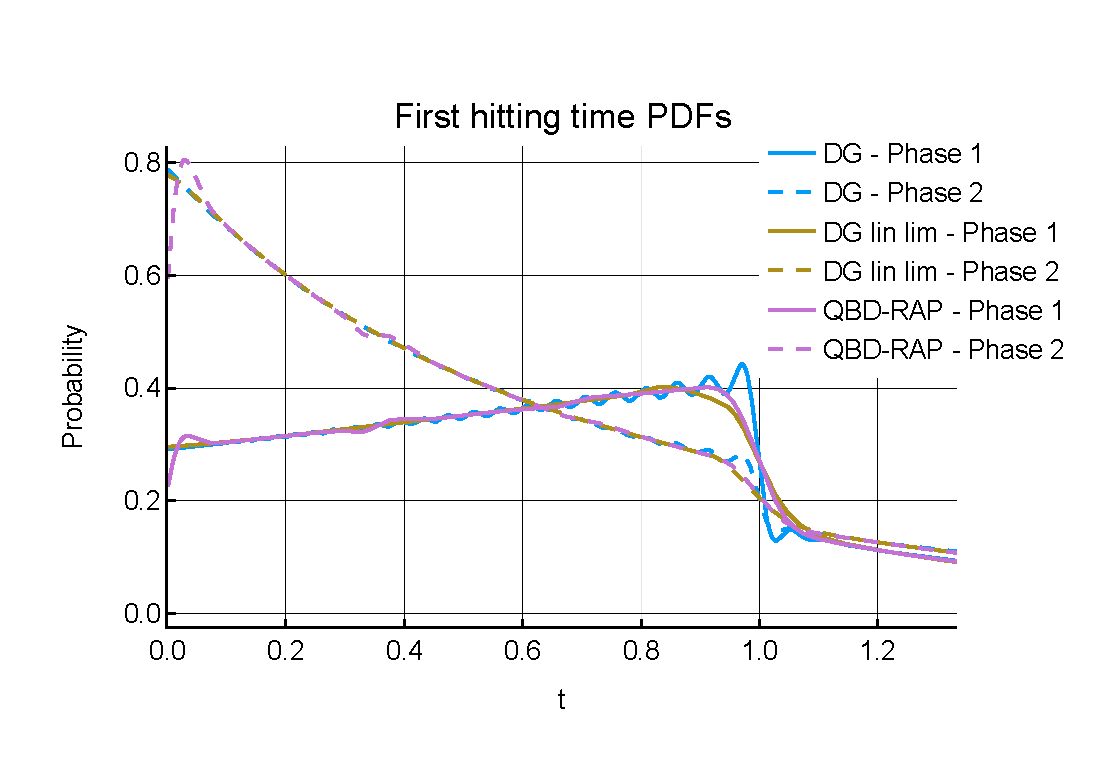
\includegraphics[width=0.8\textwidth,trim={0cm 1.25cm 0cm 1.25cm},clip]{chapter6/figs/hitting_times_model/hitting_times/exp/pdf_order21.pdf}%
	\caption{Approximations of the PDF of the first hitting time for Model~\ref{model: simple} with the exponential initial condition. The blue lines were obtained from the dimension-21 DG scheme, the purple lines were obtained from the dimension-21 QBD-RAP scheme and the gold lines were obtained from the dimension 22 DG-lin-lim scheme. The DG scheme displays oscillations around the discontinuities at \(t=1\). The QBD-RAP scheme has oscillations near \(t=0\) and \(t=0.4\). } 
	\label{fig: hitting time oscillation exp} 
\end{figure}
%\exampleFloatBarrier
In Figure~\ref{fig: hitting time oscillation exp} there is another small oscillation present in the QBD-RAP approximation around \(t=0.35\) in both phases. The cause of this oscillation is likely related to the discussion above. Consider a sample path which starts at \(x=0.34\), just to the right of the cell-edge at \(1/3\), in Phase~1, changes phase once at time \(u\), then remains in that phase until the boundary at \(x=0\) is hit. For the fluid queue, the hitting time of this sample path is \(0.34 + 2u\). The QBD-RAP approximation to this sample paths has density
\begin{align}
	\int_{v=u}^\infty \bs \alpha e^{(\bs S - \bs I)u} \bs D e^{(\bs S - 1.1\bs I)(v-u)}\bs s \bs \alpha e^{(\bs S-1.1\bs I)w}\bs s \wrt v.\label{eqn :lf2}
\end{align}
The first term in (\ref{eqn :lf2}) is the same as the first term in (\ref{eqn :lf}), and this is likely the source of the oscillation. 


% To further comment on the approximation of a point mass by (\ref{eqn:aafba}), recall the . We found that this closing operator has difficulty approximating mass at . 


\paragraph{Point mass initial condition}
\begin{figure}[h]
	\centering
	% 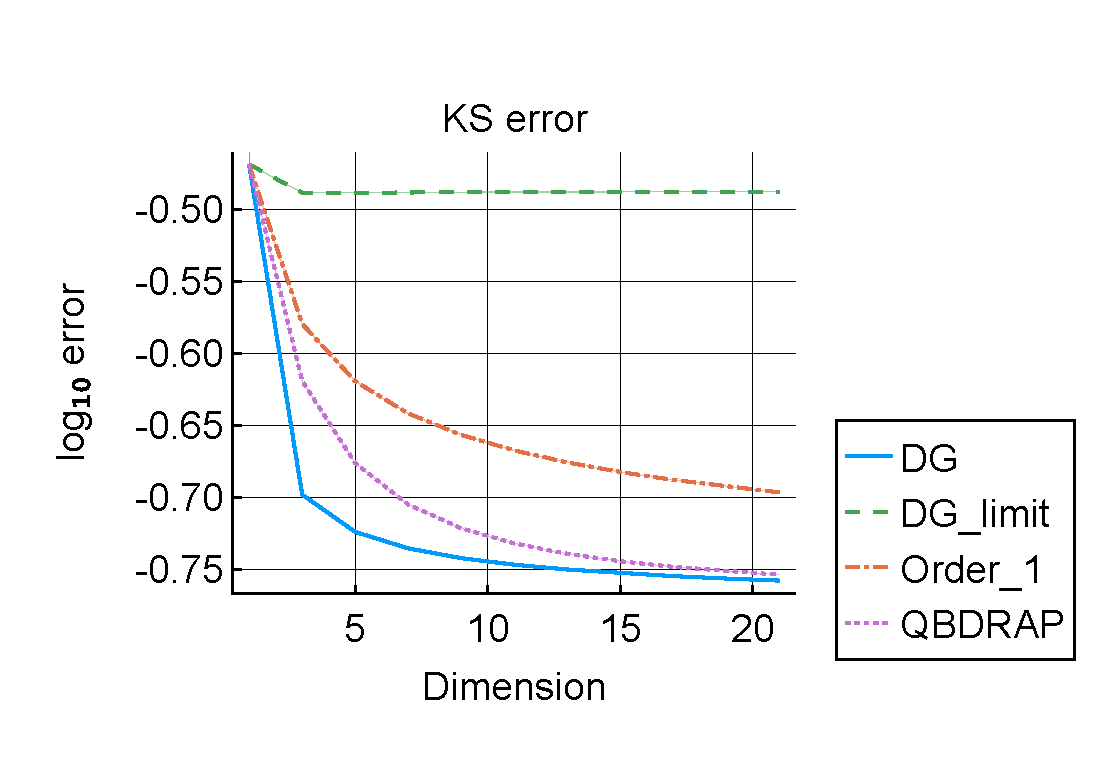
\includegraphics[width=0.5\textwidth,trim={0.75cm 0.8cm 0.25cm 1.25cm},clip]{chapter6/figs/hitting_times_model/hitting_times/point_mass/ks_error_formatted.pdf}%
	\includegraphics[width=0.5\textwidth,trim={0.75cm 0.8cm 0.25cm 1.25cm},clip]{chapter6/figs/hitting_times_model/hitting_times/point_mass/l1_cdf_error_formatted.pdf}
	% \caption{KS (left) and \(L^1\) (right) errors between the simulated and approximate first hitting time CDFs in (\ref{eqn: hit cdf}) for Model~\ref{model: simple} with the point mass initial condition. The approximations were obtained via the DG (blue solid line), DG-lim (orange dashed line), uniformisation (green dashed line), QBD-RAP (purple dotted line) and DG-lin-lim (gold dashed line) schemes. Bootstrapped 90\% confidence intervals are shown by the lighter coloured bars surrounding the lines. The black dotted lines are linear least-squares fits to the last 8 data points and the slopes of the least square lines are written next to the last point.}
	\caption{\(L^1\) errors between the simulated and approximate first hitting time CDFs in (\ref{eqn: hit cdf}) for Model~\ref{model: simple} with the point mass initial condition. The approximations were obtained via the DG (blue solid line), DG-lim (orange dashed line), uniformisation (green dashed line), QBD-RAP (purple dotted line) and DG-lin-lim (gold dashed line) schemes. Bootstrapped 90\% confidence intervals are shown by the lighter coloured bars surrounding the lines. The black dotted lines are linear least-squares fits to the last 8 data points and the slopes of the least square lines are written next to the last point.} 
	\label{fig: hitting time pm} 
\end{figure}
\begin{figure}[h]
	\centering
	\includegraphics[width=0.8\textwidth,trim={0cm 1.25cm 0cm 1.25cm},clip]{chapter6/figs/hitting_times_model/hitting_times/point_mass/cdf_order21DG_and_sims.pdf}%
	\caption{Approximations of the CDF of the first hitting time in Phase~1 for Model~\ref{model: simple} with the point mass initial condition. The blue line was obtained from the dimension-21 DG scheme, the purple dotted line from the dimension-21 QBD-RAP scheme, and the gold dashed line from the dimension 22 DG-lin-lim scheme. The empirical CDF obtained via simulation is plotted as the teal dashed line. The DG scheme displays negative approximations to probabilities. } 
	\label{fig: hitting time oscillation} 
\end{figure}
Figure~\ref{fig: hitting time pm} shows the \(L^1\) error for the CDF for the five numerical approximation schemes applied to the hitting time problem with the point mass initial condition. Due to the discontinuity the KS error is not very insightful for this problem. 

Observing Figure~\ref{fig: hitting time pm}, the DG-lim scheme does not appear to converge, suggesting oscillations in the DG approximation as we might expect given the discontinuity. Of the other positivity preserving schemes, the uniformisation, DG-lin-lim and QBD-RAP schemes all appear to converge, with the QBD-RAP converging fastest and the DG-lin-lim and uniformisation schemes performing similarly. 

The error for the DG scheme reduces significantly between dimension 1 and dimension 3, then reduces at a slower rate after that. For dimension 3 and above the DG scheme approximates the smooth regions of the solution well and the majority of the error is from the region around the discontinuity, which reduces at a slower rate. The DG scheme appears to perform best, however, oscillations are present in the DG approximation. In Figure~\ref{fig: hitting time oscillation} we plot the CDFs of the hitting time for Phase~1 obtained via the DG and QBD-RAP schemes, each using a dimension 21 basis, and for the DG-lin-lim scheme with dimension 22. Observing Figure~\ref{fig: hitting time oscillation} the DG approximation displays oscillations around the discontinuity at \(t=1\) while the other two schemes do not. Of the two positivity preserving schemes in Figure~\ref{fig: hitting time oscillation}, the QBD-RAP scheme appears to approximate the discontinuity best. 


\subsection*{Summary}
The results of this experiment are somewhat similar to the last experiment on transient distributions; the DG-lim scheme performs poorly, the DG scheme exhibits oscillations, of the three other positivity preserving schemes, the uniformisation scheme performs poorest, while the QBD-RAP and DG-lin-lim schemes perform similarly, with the QBD-RAP scheme performing slightly better for the point mass initial condition and the DG-lin-lim scheme performing slightly better for the exponential initial condition. 

\FloatBarrier
\section{First-return distributions of fluid-fluid queues}\label{sec: ffq num}
Now consider the fluid-fluid queue first analysed in \cite{blnos2022} which is a modified version of a model first presented in \cite{lnp13}. We refer the reader to \cite{blnos2022} for more on the DG scheme applied to this model. 
\begin{model}\label{model: ffq}
	Consider a stochastic fluid-fluid queue $\{(\dot W(t),X(t),\varphi(t))\}_{t\geq0},$ where $\{X(t)\}$ and $\{\dot W(t)\}$ represent the workloads in Buffers~1 and~2 at time $t \geq 0$, respectively, both driven by the phase $\{\varphi(t)\},$ which is a Markov chain on the state space $\mathcal{S} = \{11,10,01,00\}$. Both $\{X(t)\}$ and $\{\dot W(t)\}$ have a regulated boundary at 0. Here, the state $11$ indicates inputs to both buffers being \textnormal{\textsc{on}}, the state $00$ indicates both being \textnormal{\textsc{off}}, the state $10$ is when only the first input is \textnormal{\textsc{on}}, and the state $01$ is when only the second is \textnormal{\textsc{on}}. The input of Buffer~$k$ is switched from \textnormal{\textsc{on}} to \textnormal{\textsc{off}} with rate $\gamma_k$, and from \textnormal{\textsc{off}} to \textnormal{\textsc{on}} with rate $\beta_k$, for $k = 1, 2$. Thus, the infinitesimal generator $T$ for $\varphi(t)$ is given by 
	\begin{align*} 
		T = \left[ \begin{array}{cccc} -(\gamma_1 + \gamma_2) & \gamma_2 & \gamma_1 & 0 \\
							\beta_2 & -(\gamma_1 + \beta_2) & 0 & \gamma_1 \\
							\beta_1 & 0 & -(\gamma_2 + \beta_1) & \gamma_2 \\
							0 & \beta_1 &\beta_2 &-(\beta_1 + \beta_2)
	\end{array}\right].
	\end{align*} 

	The net rates of change for $X(t)$, denoted $c_i$, are given by 
	% 
	\begin{align*} 
	& (c_{11},c_{10},c_{01},c_{00})   =  \begin{array}{rrrr} 
	(\lambda_1-\theta_1,  & \lambda_1 -\theta_1, &  -\theta_1, & -\theta_1),
	\end{array}  
	\end{align*} 
	% 
	and the net rates of change for $\dot W(t)$, denoted $r_i$, are as follows  
	%  
	\begin{align*} 
	(r_{11},r_{10},r_{01},r_{00})  & = \left\{ \begin{array}{lrrrll}  
	% (\lambda_2 -\kappa, & \;\;\;\;0, & \lambda_2 - \kappa, &  \;\;\;\;0) & \text{if } X_t = 0,  W_t = 0,\\
	%  \vspace*{-0.3cm} \\
												(\lambda_2 - \kappa, & \;\;\;-\kappa,  & \lambda_2 - \kappa, & -\kappa) &\text{if } X_t = 0, \\
												\vspace*{-0.3cm} \\
	%	(\lambda_2 -\theta_2,  &  0,  & \lambda_2 - \theta_2,  & \;\;\;\; 0) & \text{if } X_t \in (0,x^*), W_t = 0,\\
	%											  \vspace*{-0.3cm} \\
		(\lambda_2 - \theta_2, & -\theta_2, & \lambda_2 - \theta_2, & -\theta_2) & \text{if } X_t \in (0,x^*),\\
												\vspace*{-0.3cm} \\
		(\;\;\;\;\;\;\; \lambda_2, & \;\;\;\;0, & \lambda_2, &  \;\;\;\;0) & \text{if } X_t \geq x^*. \end{array}
												\right.
	\end{align*} 

	For our numerical experiments, we use the parameter choices given in~\citep{lnp13}: 
	% 
		\begin{align} 
			\label{eqn:parameters}
		\gamma_1 & =11, \quad  \beta_1 = 1, \quad \lambda_1 = 12.48, \quad  \theta_1 = 1.6, \quad  \kappa = 2.6, \\
			\label{eqn:parameters-2}
		\gamma_2 & = 22, \quad \beta_2  = 1, \quad  \lambda_2 = 16.25, \quad \theta_2 = 1.0, \quad x^* = 1.6.
		\end{align} 
	We consider the initial distribution which is a point mass at \(W(0)=0,\, X(0)=5,\, \varphi(0)=01\). 
\end{model}
	
While the true problem has an unbounded domain $[0,\infty)$, the approximations require the domain of approximation to be a finite interval. Here we choose an upper bound of \(b=48\) and place a regulated boundary at the upper boundary. The effect of this truncation can be partly quantified by evaluating \(\lim\limits_{t\to\infty}\mathbb P\left(X(t) > 48\right)\approx 5.83 \times 10^{-9}\). 

We obtain approximations to the generator of the fluid queue \(\{(X(t),\varphi(t))\}\) via the DG, QBD-RAP and uniformisation schemes. We do not apply slope limiting in this case as slope limiting results in a non-linear operator which means slope limiting schemes cannot be used to approximate the operator-Riccati equation by a matrix-Riccati equation. All the discretisations use a cell width of \(\Delta=0.4\). The approximate generator matrix is then used to approximate the first-return operator \(\mathbb\Psi(s)\) as discussed in Section~\ref{sec: intro Psi}. As in Section~\ref{sec: intro Psi}, let \(\bs{B}^{m,n}\), \(m,n\in\{+,-,0\}\) be an approximation to \(\mathbb B^{m,n},\, m,n\in\{+,-,0\}\) of dimension \(p\), and recall that \(\bs{D}^{n,m},\,m,n\in\{+,-\}\) is given by 
\[\bs D^{m,n} = \bs{R}^m (\bs{B}^{m,n} + \bs{B}^{m,0}(\bs B^{0,0})^{-1}\bs{B}^{0,n}), \, m,n\in\{+,-\}, \]
where \(\bs R^m\) is a diagonal matrix with diagonal blocks \(1/r_i^k\bs{I}_p\), \(i\in\calS_k^m\), \(k\in\mathcal K^m\), where \(r_i^k\) is the (constant) value of \(r_i\) on cell \(k\).
Then \(\bs{\Psi}\), an approximation to \(\mathbb \Psi\), is given by the solution to the matrix-Ricatti equation 
\begin{align}\label{eqn:RiccatiPsi2}
    \bs D^{+-}
+ \bs \Psi   \bs D^{-+}\bs \Psi
+   \bs D^{++}\bs \Psi
+ \bs \Psi  \bs D^{--}
= \bs 0.
\end{align}
Due to the stochastic interpretation of the uniformisation and QBD-RAP schemes the approximations to \(\mathbb \Psi(s)\) have a stochastic interpretation as the first-return probabilities of a fluid queue driven by a CTMC and QBD-RAP, respectively (see \cite[Chapter~7]{p2019} and \cite{bgnp2021} for details on the latter). For the DG scheme the approximation of \(\mathbb \Psi(s)\) is not as well-understood. Here, we assume that it is given by the solution to (\ref{eqn:RiccatiPsi2}) and is a polynomial approximation. %\footnote{I believe that the resulting operator is a projection operator which, given an initial distribution, projects the distribution of \(X(\zeta_{W}(\{0\}))\) on to a set of polynomial basis functions, much like the DG method itself.}

Ultimately, we approximate the first-return distribution 
\begin{align}\label{eqn: first return Y 1}
	\mathbb P(X(\zeta_{W}(\{0\}))\leq x, \varphi(\zeta_{W}(\{0\}))=i\mid \bs X(0)\sim \mu),
\end{align}
where we recall \(\zeta_{W}(E) = \inf\{t>0\mid \dot W(t)\in E\}\) is the first hitting time of \(\{\dot W(t)\}\) on the set \(E\). For Model~\ref{model: ffq}, it is only possible for the process \(\dot W(t)\) to return to \(0\) at time \(t\) when \((X(t),\varphi(t))\in[0,1.6)\times \{10,00\}\), so we evaluate the approximations over this region only. We use a grid of 10,001 points on which we evaluate the approximations of the CDF in each phase. 

For a `ground truth' comparison, we simulated \(5\times 10^{10}\) realisations of the fluid-fluid queue and recorded the value of \(\{X(t)\}\) and \(\{\varphi(t)\}\) at the time of first return of the second fluid, \(\{\dot W(t)\}\). The empirical approximation of (\ref{eqn: first return Y 1}) was then constructed, and error metrics for the difference between the empirical CDF and the approximations were computed. To account for Monte-Carlo errors we used a bootstrap with 1,000 bootstrap samples to construct 1,000 bootstrap samples of the error estimates and ultimately estimated the 5th and 95th percentiles of the error distribution. Each of the 1,000 bootstrap samples was constructed by resampling the original \(5\times 10^{10}\) realisations \(5\times 10^{10}\) times with replacement.

\begin{figure}[h]
	\centering
	\includegraphics[width=0.5\textwidth,trim={0.75cm 0.8cm 0.25cm 1.25cm},clip]{chapter6/figs/ffq/cts/ks_error_formatted.pdf}%
	\includegraphics[width=0.5\textwidth,trim={0.75cm 0.8cm 0.25cm 1.25cm},clip]{chapter6/figs/ffq/cts/l1_cdf_error_formatted.pdf}
	\caption{KS (left) and \(L^1\) (right) errors between the simulated and approximate CDFs of \(X(\zeta_{W}(\{0\}))\) in (\ref{eqn: first return Y 1}) for Model~\ref{model: ffq}. The approximations were obtained via the DG (blue solid line), uniformisation (green dashed line) and QBD-RAP (purple dotted line) schemes. Bootstrapped 90\% confidence intervals are shown by the lighter coloured bars surrounding the lines. The black dotted lines are linear least-squares fits to the last 8 data points and the slopes of the least square lines are written next to the last point.} 
	\label{fig: ffq return cts} 
\end{figure}
\begin{figure}[h]
	\centering
	\includegraphics[width=0.5\textwidth,trim={0.75cm 0.8cm 0.25cm 1.25cm},clip]{chapter6/figs/ffq/cts/l1_cell_probs_error_formatted.pdf}%
	\caption{Cell-wise errors between the simulated and approximate probabilities of \(X(\zeta_{W}(\{0\}))\) residing on each cell \(\mathcal D_k\) or at the boundary for Model~\ref{model: ffq}. The approximations were obtained via the DG (blue solid line), uniformisation (green dashed line) and QBD-RAP (purple dotted line) schemes. Bootstrapped 90\% confidence intervals are shown by the lighter coloured bars surrounding the lines. The black dotted lines are linear least-squares fits to the last 8 data points and the slopes of the least square lines are written next to the last point.} 
	\label{fig: ffq cell probs} 
\end{figure}
%\exampleFloatBarrier
In Figures~\ref{fig: ffq return cts} and~\ref{fig: ffq cell probs} we plot the error metrics for the approximations to the distribution~(\ref{eqn: first return Y 1}). The DG scheme performs best converging rapidly until the error in the approximation scheme is swamped by other numerical (simulation) errors\footnote{There are a significant number of other sources of error here; the largest contribution to error is simulation, but also machine precision errors, errors in solving the matrix Riccati equation to approximate \(\mathbb \Psi(s)\), errors from approximating error metrics (numerical integration/finding KS statistic), errors from approximating the initial condition and truncation errors. Furthermore, for the QBD-RAP, since the parameters \(\bs \alpha,\,\bs S,\,\bs s\,\) and \(\bs D\) are found numerically, then there is another source of error from this.}. The QBD-RAP scheme is second best and the uniformisation scheme appears to be the slowest to converge. Here, the first return distribution appears to be smooth, hence we might expect the DG scheme to perform well. The initial condition, however, is not smooth and the DG approximation violates the axioms of probability for the initial distribition. Interestingly, however, there is no sign of this in the first return distribution. 
 

By modifying Model~\ref{model: ffq} slightly, we can construct a first return distribution which is discontinuous. 
\begin{model}\label{model: ffq2}
	Consider a fluid-fluid queue which is the same as Model~\ref{model: ffq} except 
	\begin{align}
		r_{00}(X(t)) = \begin{cases}
			-\kappa, & \mbox{ if }X(t)=0,\\
			-\theta_2, & \mbox{ if }X(t)=\in(0,x^*),\\
			\theta_2, & \mbox{ if }X(t)\geq x^*,
		\end{cases}
	\end{align}
	with an initial distribution which is a point-mass at \(W(0)=0,\, X(0)=2, \varphi(0)=00\). 
\end{model}
As before, we use the DG, uniformisation and QBD-RAP schemes to approximate the model, and compare the approximations to simulations. 

Consider a sample path of Model~\ref{model: ffq2} which begins at \(X(0)=2\) in Phase~\(00\) and remains in Phase~\(00\) until a time \(t>0.5\). On this sample path, at time \(u\leq 0.5\) the position of the first fluid level is \(X(u)=2-1.6u\). Moreover, for \(u\in[0,0.25]\), \(X(u)\geq x^*\) and \(r_{00}(X(u))=\theta_2=1>0\), and for \(u\in(0.25,0.5]\), \(X(u)\in(0,x^*)\) and \(r_{00}(X(u))=-\theta_2=-1<0\). Hence, for \(u\leq 0.5\) the second fluid level is \(W(u)=u1(u\leq 0.25)+(0.25-u)1(u>0.25)\) and at time \(u=0.5\), the second fluid level first returns to \(0\), i.e.~\(\zeta_{W}(\{0\})=0.5\) on this sample path. The probability of this sample path is \(e^{-(\beta_1+\beta_2)\times 0.5}\). Thus, in the distribution of the first return time of the second fluid level there is a point mass at \(u=0.5\) with magnitude \(e^{-(\beta_1+\beta_2)\times 0.5}\). Furthermore, on the same sample path \(X(\zeta_W(\{0\}))=X(0.5)=1.2\), and hence there is a point mass with magnitude \(e^{-(\beta_1+\beta_2)\times 0.5}\) in the distribution of \(X(\zeta_W(\{0\}))\) also. 

\begin{figure}[h]
	\centering
	\includegraphics[width=0.5\textwidth,trim={0.75cm 0.8cm 0.25cm 1.25cm},clip]{chapter6/figs/ffq/discts/ks_error_formatted.pdf}%
	\includegraphics[width=0.5\textwidth,trim={0.75cm 0.8cm 0.25cm 1.25cm},clip]{chapter6/figs/ffq/discts/l1_cdf_error_formatted.pdf}
	\caption{KS (left) and \(L^1\) (right) errors between the simulated and approximate CDFs of \(X(\zeta_{W}(\{0\}))\) (Equation~\ref{eqn: first return Y 1}) for Model~\ref{model: ffq2}. The approximations were obtained via the DG (blue solid line), uniformisation (green dashed line) and QBD-RAP (purple dotted line) schemes. Bootstrapped 90\% confidence intervals are shown by the lighter coloured bars surrounding the lines. The black dotted lines are linear least-squares fits to the last 8 data points and the slopes of the least square lines are written next to the last point.} 
	\label{fig: ffq return discts} 
\end{figure} 
% \begin{figure}[h]
% 	\centering
% 	\includegraphics[width=0.5\textwidth,trim={0.75cm 0.8cm 0.25cm 1.25cm},clip]{chapter6/figs/ffq/discts/l1_cell_probs_error_formatted.pdf}%
% 	\caption{Cell-wise error between the simulated and approximated probabilities of \(X(\zeta_{Y}(\{0\}))\) residing in each cell \(\mathcal D_k\) or at the boundary for Model~\ref{model: ffq2}. The approximations were obtained via the DG (blue solid line), uniformisation (green dashed line) and QBD-RAP (purple dotted line) schemes. Bootstrapped 90\% confidence intervals are shown by the lighter coloured bars surrounding the lines. The black dotted lines are linear least-squares fits to the last 8 data points and the slopes of the least square lines are written next to the last point.} 
% 	\label{fig: ffq2 cell probs} 
% \end{figure}
\begin{figure}[h] 
	\centering
	\includegraphics[width=0.8\textwidth,trim={0cm 1.25cm 0cm 1.25cm},clip]{chapter6/figs/ffq/discts/phase_4_cdf.pdf}%
	\caption{Approximations of the CDF of the distribution of \(X\) at the time \(\zeta_W(\{0\})\) in Phase~1 for Model~\ref{model: ffq2}. The blue line was obtained from the dimension-21 DG scheme, the purple dotted line from the dimension-21 QBD-RAP scheme, and the gold dotted line is the empirical CDF obtained via simulation. The DG scheme displays oscillations around the discontinuity, which mean that is does not represent a CDF.} 
	\label{fig: ffq2 oscillation} 
\end{figure}
Figure~\ref{fig: ffq return discts} plots error metrics for the first return distribution. Note that due to the discontinuity, the KS error is bounded below in how small it can be. The approximations all give a continuous approximation to the CDF, hence the smallest possible KS error is 1/2 the size of the discontinuity, which is \(\approx 0.184\) here. Observing Figure~\ref{fig: ffq return discts} we see that the DG scheme performs well, followed by the QBD-RAP scheme, then the uniformisation scheme performs worst. However, the DG scheme results in an oscillatory solution which does not represent a CDF, as shown in Figure~\ref{fig: ffq2 oscillation}.


\subsection{Summary}
Although the initial condition in the DG scheme violated the axioms of probability, for the smooth problem the DG scheme was highly effective, significantly outperforming the positivity preserving QBD-RAP and uniformisation methods. Interestingly the oscillations in the initial condition were not present in the first return distribution. 

For the discontinuous problem, the DG scheme displayed oscillations (in both the initial condition and first-return distribution) and did not produce a legitimate CDF, but it did produce the lowest errors. Of the positivity preserving methods (QBD-RAP and uniformisation scheme), the QBD-RAP scheme performed the best for both problems. 
\FloatBarrier


\section{Discussion}
In this chapter we have numerically investigated some properties of the QBD-RAP approximation scheme and compared it to existing schemes; the uniformisation scheme of \cite{bo2013} and the discontinuous Galerkin scheme. In general, the numerical experiments show that the smoother the problem is, the better the performance of the DG scheme, and it emphatically outperforms the other two schemes for smooth problems. However, for problems with discontinuities the DG approximation can exhibit oscillations and result in illegitimate approximations to probability distributions which violate the axioms of probability. The QBD-RAP and uniformisation approximations are guaranteed to produce legitimate distributions and, of the two, the QBD-RAP scheme almost always produces lower errors. 

To avoid the problems of oscillations we can sometimes employ a \emph{slope limiter} with the DG scheme which reduces the scheme to linear in the regions where oscillations are detected. We implemented two slope-limited DG schemes, the DG-lim scheme which takes a high order DG scheme and limits the solution as necessary, and the DG-lin-lim, which is a linear approximation on a finer grid designed to use approximately the same computational resources as the other schemes considered. The numerical experiments demonstrate a significant loss of accuracy in the approximation when a DG-lim scheme is used for discontinuous problems. We conclude that the DG-lim scheme is not a viable scheme for the discontinuous problems considered here. The numerical experiments suggest that the DG-lin-lim scheme can perform well, and is similar to the performance of the QBD-RAP scheme, in the presence of discontinuities. %For highly discontinuous problems (i.e.~problems with point masses) the QBD-RAP scheme can outperform the DG-lin-lim scheme. %For the application of the schemes to fluid-fluid queues, there is no obvious way to apply the concept of a slope limiter. %When the slope limiter detects oscillations in the approximate solution, it reduces the DG scheme to linear in the region surrounding the oscillations, otherwise, the slope limiter leaves the solution unchanged. Thus, the slope limiter permits high-order approximations away from oscillations, while also removing oscillations. 

As a first step, in Section~\ref{sec: recon num}, we examined the ability of each scheme to approximate various initial conditions. For the DG scheme, this is equivalent to a projection of the initial condition on to a set of basis polynomials, for the uniformisation scheme this is equivalent to projecting the initial condition on to a basis of constant functions, and for the QBD-RAP scheme the approximation of the initial condition is as described in Sections~\ref{sec: initial conditions} and~\ref{sec: closing}. Section~\ref{sec: comp} demonstrates that the DG scheme (projection) can result in oscillations and negative regions in the approximation when the initial condition is discontinuous. The uniformisation and QBD-RAP schemes avoid this, but appear to have higher errors and the QBD-RAP scheme appears to have the largest errors. For discontinuous initial conditions the rates of convergence are comparable for all three schemes. When the initial condition to be approximated is sufficiently smooth, then the DG approximation is superior. The QBD-RAP scheme performed the poorest for the examples considered. %However, once dynamics are introduced into the problem the approximation from the QBD-RAP scheme can be more accurate than that of the uniformisation scheme suggesting that the QBD-RAP scheme is better able to resolve the movement of probability between cells, as demonstrated in Section~\ref{sec: wave num}.

Next, in Section~\ref{sec: wave num}, we investigated the performance of approximations for a simple travelling wave model with various initial conditions. The travelling wave model is useful as it allows us to investigate the ability of the schemes to capture the flow of probability without stochastic dynamics and, since the solution is known, there is no need for simulation. With the travelling wave model we demonstrate that, for problems with discontinuities, the DG scheme can display oscillations and violate the axioms of probability, while the other schemes (DG-lim, DG-lin-lim, uniformisation and QBD-RAP schemes) avoid oscillations. For discontinuous problems the rates of convergence of the QBD-RAP and DG-lin-lim schemes is similar. Interestingly, even though the QBD-RAP scheme performed worst for approximating initial conditions in the previous section, it outperformed the uniformisation scheme for this model, demonstrating that the QBD-RAP scheme can capture the dynamics of the flow of probability better than the uniformisation scheme. For smooth problems the DG scheme is superior.

We then investigated the performance of the approximations on a simple fluid queue with two phases. First, in Section~\ref{sec:stat}, we looked at the limiting distribution, which is known to be smooth. Since the problem is smooth, then the DG scheme was superior as expected. Of the uniformisation and QBD-RAP schemes, the QBD-RAP scheme gives more accurate solutions. 

In Section~\ref{sec: transient approx} we turned our attention to approximating transient distributions for the same model and considered two different initial conditions, a point-mass and an exponential initial condition. The discontinuous initial condition results in a discontinuous transient distribution. As for the exponential initial condition, this example demonstrates that, even if the initial condition appears `nice', it can still result in non-smooth (i.e.~non-differetiable) solutions. The numerical evidence suggests that the lack of smoothness in the problem with the exponential initial condition is not problematic for the DG scheme, however, the DG scheme exhibits severe oscillations for the problem with the discontinuous initial condition. For both initial conditions, the DG-lim scheme detects oscillations and reduces the approximation to linear which renders the scheme not viable for these problems. Of the uniformisation, DG-lin-lim and QBD-RAP schemes, the latter two perform similarly, and better than the uniformisation scheme. Of the DG-lin-lim and QBD-RAP schemes the QBD-RAP scheme performed better in the presence of a point mass while the DG-lin-lim scheme performed better with the exponential initial condition.

Section~\ref{sec: hit approx} investigated the performance of the schemes for approximating the hitting time distribution for the same fluid queue with two initial conditions, an exponential initial condition and a point-mass. For this problem there is never any in-flow of mass at the boundaries of the interval and so, for a solution to be continuous, the initial condition needs to be chosen carefully, otherwise discontinuities in the transient distribution may result, as was the case for both initial conditions considered here. The numerical results suggest that, due to discontinuities in the problems, the DG scheme may display oscillations and violate the axioms of probability. Since the uniformisation, DG-lin-lim, and QBD-RAP schemes can handle discontinuities, they perform suitably, with the QBD-RAP and DG-lin-lim schemes performing similarly and better than the uniformisation. 

Lastly, we applied the DG, uniformisation and QBD-RAP schemes to two simple fluid-fluid queues in Section~\ref{sec: ffq num}. In the first fluid-fluid queue, which appears to have a smooth first return distribution, the DG scheme performs very well (however, the initial condition for the DG scheme displayed oscillations). Of the two positivity preserving schemes considered, the QBD-RAP scheme performs better than the uniformisation scheme. In the second example, which has a discontinuity in the first return distribution, the DG scheme produces the lowest errors, but exhibits oscillations in the solution. The QBD-RAP and uniformisation schemes do not produce oscillations and, of the two, the QBD-RAP scheme performs best. Moreover, when computing approximations to the first-return operator of a fluid-fluid queue in Section~\ref{sec: ffq num}, the QBD-RAP and uniformisation schemes lead to an algorithm that is theoretically justified. In contrast, to-date there no theory surrounding the DG approximation to the same operator (let alone any positivity preserving variants of the DG scheme).

%As we mentioned in the introduction to this chapter, in Sections~\ref{sec: recon num}, \ref{sec:stat}, and \ref{sec: ffq num} slope limiting is not used as it is not applicable: in these cases slope limiting is practically equivalent to post-processing the solution by detecting oscillations, then projecting oscillatory regions of the solution onto a basis of linear functions, and making some corrections to the solution if it happens to be negative.



In conclusion, when the problem is known to be smooth, the DG scheme is very likely to produce excellent results. However, for discontinuous problems, the scheme can show oscillations and may lead to illegitimate approximations to distribution functions which violate the axioms of probability. The slope limiter overcomes this, but reduces the accuracy of the DG scheme to linear near discontinuities, sometimes severely affecting the quality of the approximation. A piecewise-linear DG scheme with a limiter, such as the DG-lin-lim scheme considered here, can produce satisfactory results for some problems. The uniformisation and QBD-RAP schemes are other alternative approximation schemes which avoid oscillatory solutions and guarantee a legitimate approximation to distributions of fluid queues. Of the uniformisation and QBD-RAP schemes, the latter often produced lower errors and performed similarly to the DG-lin-lim scheme. Moreover, the uniformisation and QBD-RAP schemes have stochastic interpretations which can aid in their analysis. For the application to fluid-fluid queues in this chapter the stochastic interpretation is important as it justifies (and defines) an approximation to the first return operator. For the DG scheme there is no such theory (that the author is aware of) and this means that the approximation to the first return operator using the DG scheme is not a rigorously defined object. On a similar note, the uniformisation and QBD-RAP schemes result in operators which are linear, whereas the DG-lim and DG-lin-lim schemes do not result in linear operators. When approximating the Riccati equation for the first return operator this is necessary as the uniformisation and QBD-RAP schemes result in a matrix-Riccati equation which can be easily solved in software, whereas slope-limited DG schemes do not lead to matrix formulations as they are non-linear. In summary, the QBD-RAP and DG-lin-lim schemes perform similarly and guarantee solutions which obey the axioms of probability, however approximating operators of fluid-fluid queues is justified when using the QBD-RAP scheme, it is not justified for the DG-lin-lim (or DG schemes in general). 
